\chapter{Timed-arc workflow nets}\label{chapter:c4}
\markboth{Chapter~\ref{chapter:c4}.}{}

%%This chapter presents a visual model for the representation of electronic contracts. It is based on a hierarchical tree diagram used to specify the contract clauses. We call this diagram \textit{Contract-Oriented Diagram} or \textit{C-O Diagram} for short. First, an informal description of the diagram is provided, describing the different elements that compose the model. Next, the diagram syntax and semantics are defined, where the semantics consists of a translation of the diagram into a network of timed automata, so the UPPAAL tool can be used for validation and verification of the e-contract model. A case study concerning an e-contract about an online auctioning process is presented, showing the usefulness of the approach. Finally, some alternative work related to \codiag\ is described.
%%
%%%%%Model description%%%
%%\section{\codiag\ Description}\label{Description}
%%\markright{~\ref{Description} \codiag\ Description}
%%
%%%%Basic Element%%
%%In Figure \ref{goal} we show the basic element of \codiag. It corresponds to a contract clause and we call it \textbf{box}. This box consists of four elements, allowing us to specify deontic norms, reparations and any restriction. There are also a name and an agent associated to the box. The \textit{name} is useful both to describe the clause and to reference the box from other clauses, so it cannot be repeated. The \textit{agent} can be used to indicate which one of the participants in the contract is affected by the clause in the box.
%%
%%\begin{figure}
%%\begin{center}
%%  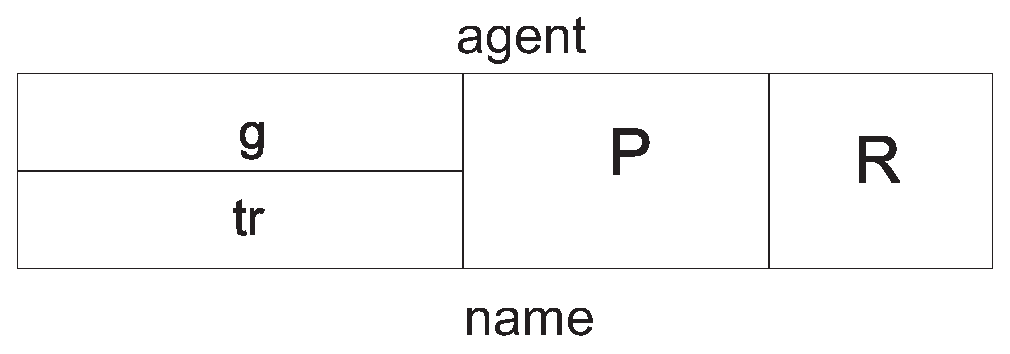
\includegraphics[width=7cm]{Figures/goal.eps}
%%\end{center}
%%  \caption{Box structure}
%%  \label{goal}
%%\end{figure}
%%
%%On the left-hand side of the box we specify the conditions and restrictions. The \textit{guard} \textbf{g} contains the conditions under which the contract clause must be taken into account. The \textit{time restriction} \textbf{tr} specifies the time frame in which the contract clause must be satisfied.
%%
%%The \textit{propositional content} \textbf{P}, on the centre, is the main element of the box, and it is used to specify deontic operators (obligations, permissions and prohibitions) that are applied over actions and the actions themselves.
%%
%%The last element of these boxes, on the right-hand side, is the \textit{reparation} \textbf{R}. This reparation, if specified by the contract clause, is another contract that must be satisfied in case the main norm is not satisfied, considering the clause eventually satisfied if this reparation is satisfied.
%%
%%%%Refinements%%
%%These basic elements of a \textit{C-O Diagram} can be refined by using AND/OR refinements, as shown in Figure \ref{refinem}, in the same way that we refine goals into subgoals in goal model diagrams \cite{Lamsweerde1993}. The aim of these refinements is to capture the hierarchical clause structure followed by most contracts. An \textbf{AND-refinement} means that all the subclauses must be satisfied in order to satisfied the parent clause. An \textbf{OR-refinement} means that it is only necessary to satisfy one of the subclauses in order to satisfy the parent clause, so we can choose which one to fulfil (exclusive or). In this way, we can build a hierarchical tree with the clauses defined by the contract, where the leaf clauses correspond to the atomic clauses, that is, to the clauses that cannot be divided into subclauses.
%%
%%\begin{figure}
%%\begin{center}
%%  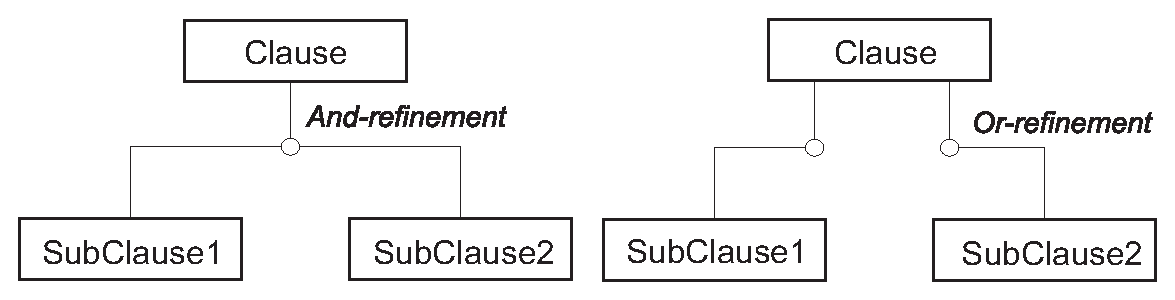
\includegraphics[width=10cm]{Figures/AndOrRefinement.eps}
%%\end{center}
%%  \caption{AND/OR refinements}
%%  \label{refinem}
%%\end{figure}
%%
%%It is also possible to use another refinement to specify a temporal relationship of sequence between the subclauses, as shown in Figure \ref{sequence}. We call it \textbf{SEQ-refinement} and it means that the norm specified in the target box (\textit{SubClause2} in Fig. \ref{sequence}) must be fulfilled after satisfying the norm specified in the source box (\textit{SubClause1} in Fig. \ref{sequence}).
%%
%%\begin{figure}
%%\begin{center}
%%  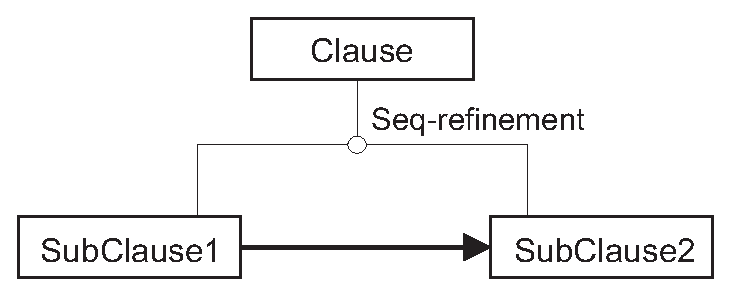
\includegraphics[width=7cm]{Figures/AndRefinementSequence.eps}
%%\end{center}
%%  \caption{Sequence refinement}
%%  \label{sequence}
%%\end{figure}
%%
%%Finally, there is another structure that can be used to model \textbf{repetition}, apart from the refinements previously defined. This structure is represented as an arrow going from a subclause to one of its ancestor clauses (or to itself), meaning the repetitive application of all the subclauses of the target clause after satisfying the source subclause. For example, in Figure \ref{Recursion} we have an \textbf{OR-refinement} with an arrow going from \textit{SubClause1} to \textit{Clause}. It means that after satisfying \textit{SubClause1} we apply \textit{Clause} again, but not after satisfying \textit{SubClause2}.
%%
%%\begin{figure}
%%\begin{center}
%%  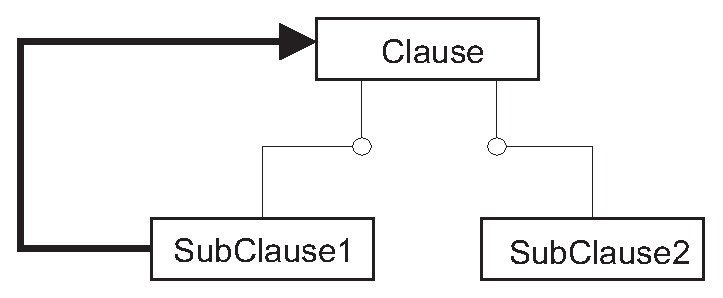
\includegraphics[width=7cm]{Figures/Recursion.eps}
%%\end{center}
%%  \caption{Repetition in \codiag}
%%  \label{Recursion}
%%\end{figure}
%%
%%%%Fields Description%%
%%In the next paragraphs we describe each one of the elements of a box/clause in more detail. For the sake of simplicity, we sometimes avoid writing all the elements of the boxes in the different figures, we just focus on the elements of interest in each case.
%%
%%\paragraph{\textbf{Propositional Content P}} This one is the main element of a box. It allows us to specify \textit{obligations}, \textit{permissions} and \textit{prohibitions} that the contract must satisfied. In this work, we follow an \textit{ought-to-do} approach \cite{Wright1999}, that is, these deontic operators are applied over \textit{actions} performed by the participants in the contract.
%%
%%We only consider the possibility of specifying \textit{atomic actions} in the \textbf{P} element of each one of the leaf clauses of our diagrams. These actions are denoted by lower case Latin letters (``a'',``b'',``c'', \ldots). We use a dash (``-'') to denote that there is no action specified in the no leaf clauses.
%%
%%The composition of actions can be achieved by means of the different kinds of refinement we have in \codiag. In this way, an AND-refinement can be used to model \textit{concurrency} ``\&'' between actions, an OR-refinement can be used to model a \textit{choice} ``+'' between actions, and a SEQ-refinement can be used to model \textit{sequence} ``;'' of actions. In Figure \ref{CompoundActions} we can see an example about how to model these compound actions through refinements, given two atomic actions \textit{a} and \textit{b}.
%%
%%\begin{figure}
%%\begin{center}
%%  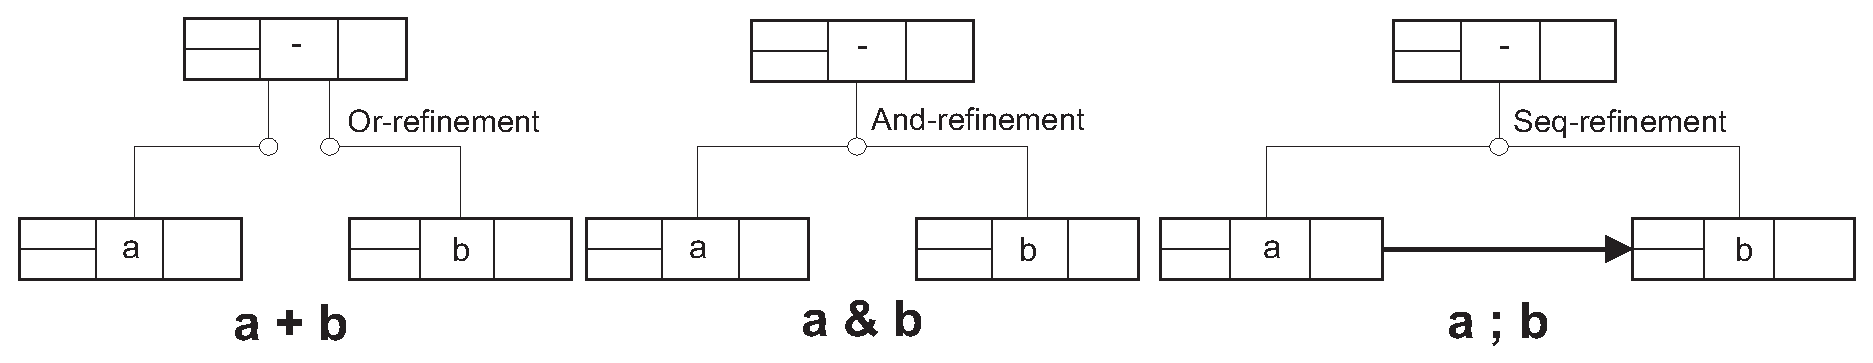
\includegraphics[width=12cm]{Figures/CompoundActions.eps}
%%\end{center}
%%  \caption{Compound actions in \codiag}
%%  \label{CompoundActions}
%%\end{figure}
%%
%%The \textit{deontic norms} (obligations, permissions and prohibitions) that are applied over these actions can be specified in any clause of our \codiag, affecting all the actions in the leaf clauses that are subclauses of this clause. If it is the case that the clause where we specify the deontic norm is a leaf clause, the norm only affects the atomic action we have in this clause. We use an upper case ``\textit{O}'' to denote an obligation, an upper case ``\textit{P}'' to denote a permission, and an upper case ``\textit{F}'' to denote a prohibition (forbidden). These letters are written in the top left corner of element \textbf{P} (Figure \ref{DeonticNorms}).
%%
%%\begin{figure}
%%\begin{center}
%%  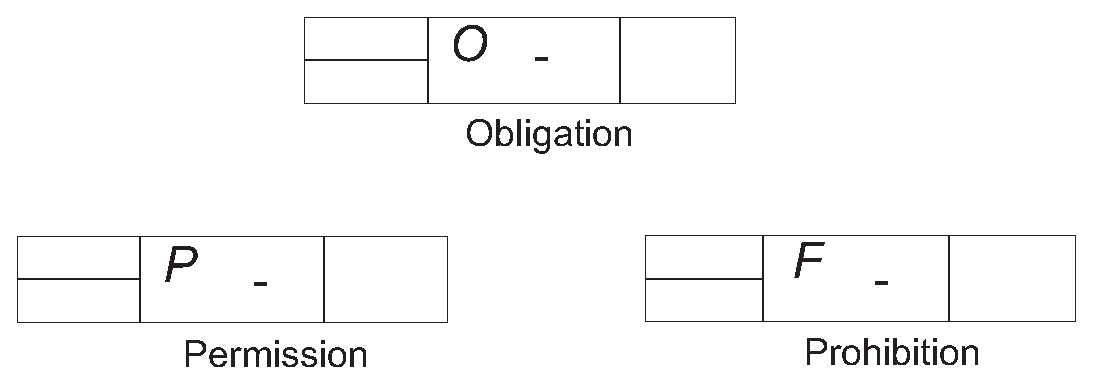
\includegraphics[width=8cm]{Figures/DeonticNorms.eps}
%%\end{center}
%%  \caption{Specification of deontic norms}
%%  \label{DeonticNorms}
%%\end{figure}
%%
%%The composition of deontic norms is also achieved by means of the different refinements we have in \codiag. Thus, an AND-refinement corresponds to the \textit{conjunction} operator ``$\wedge$'' between norms, an OR-refinement corresponds to the \textit{choice} operator ``$+$'' between norms, and a SEQ-refinement corresponds to the \textit{sequence} operator ``$;$'' between norms. For example, we can imagine having a leaf clause specifying the obligation of performing an action \textbf{a}, written as \textit{O}(a), and another leaf clause specifying the obligation of performing an action \textbf{b}, written as \textit{O}(b). These two norms can be combined in the three different ways mentioned before through the different kinds of refinement, as shown in Figure \ref{CompoundNorms}.
%%
%%\begin{figure}
%%\begin{center}
%%  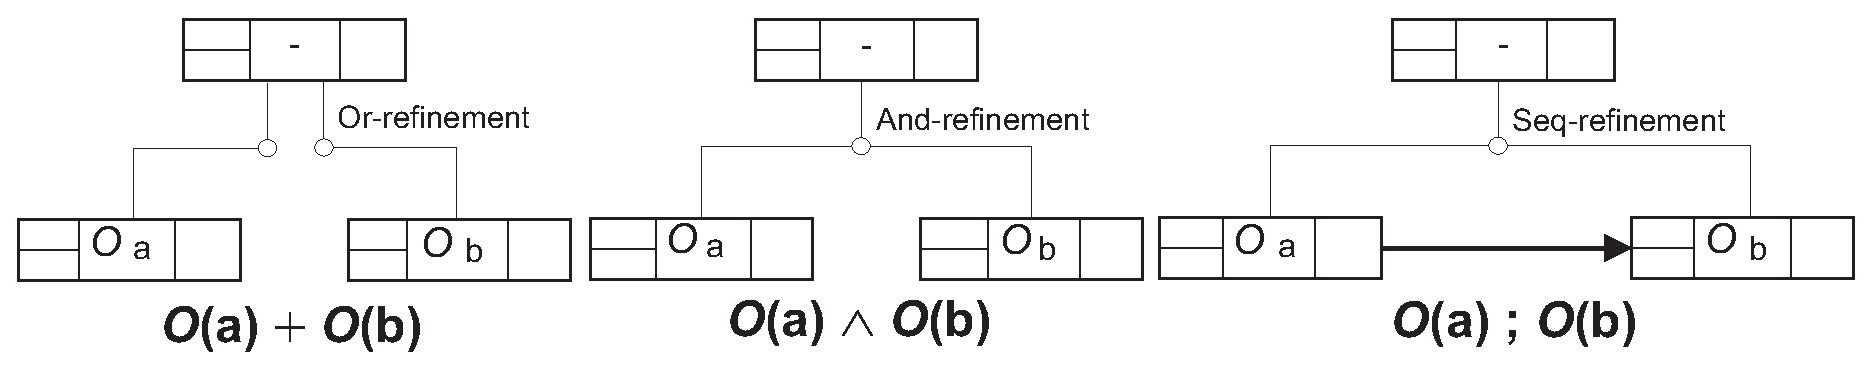
\includegraphics[width=12cm]{Figures/CompoundNorms.eps}
%%\end{center}
%%  \caption{Composition of deontic norms in \codiag}
%%  \label{CompoundNorms}
%%\end{figure}
%%
%%However, the specification of obligations, permissions and prohibitions in our diagrams must fulfil the following rules:
%%
%%{\renewcommand{\labelenumi}{\textit{\arabic{enumi}.}}
%%
%%\begin{enumerate}
%%
%%\item At least one deontic norm must be specified in each one of the branches of our hierarchical tree of clauses, i.e., we cannot have an action without a deontic norm applied over it.
%%
%%\item No more than one deontic norm can appear in each one of the branches of our hierarchical tree of clauses, i.e., we cannot have deontic norms applied over other deontic norms.
%%
%%\item The deontic norms we take into account to check restrictions \textit{1.} and \textit{2.} can be shared by several branches, i.e., when we have a deontic norm applied over a compound action, this norm is part of several branches of our hierarchical tree of clauses.
%%
%%\end{enumerate}
%%
%%}
%%
%%The \textit{repetition} of both, actions and deontic norms, can be achieved by means of the repetition structure we define in \codiag. The meaning of this structure is similar to the operator \textit{Kleene's star} ``$*$'' applied over the elements of the target clause of the arrow, but it is richer in the sense that the repetition can be conditioned to the satisfaction of the source clause of the arrow and not other alternative clause.
%%
%%To sum up, the content of element \textbf{P} in our \codiag\ change depending on the type of clause. In the \textit{leaf clauses} we must always specify an atomic action and we must also specify a deontic norm over this action if it has not been specified before in this branch of the diagram. In the \textit{no leaf clauses} we cannot specify actions, but we can specify a deontic norm whenever the rules listed before are not broken (there is not conflict with other norm and it is eventually applied over an action).
%%
%%\paragraph{\textbf{Reparation R}} This element of a box can state a \textit{new contract} that must be satisfied when the main proposition \textbf{P} is not satisfied (a \textit{prohibition} is violated or an \textit{obligation} is not fulfilled, there is not reparation for \textit{permission}). This new contract can be just a new norm, but it can also be a new hierarchical tree of clauses, including their own reparations. In this way, we are able to specify nested reparations in our \textit{C-O Diagram}.
%%
%%The element \textbf{R} is only allowed in the clauses of our diagrams where we specify a deontic norm of obligation or prohibition in element \textbf{P}, being forbidden in the rest of clauses. E.g., we can imagine a simple contract \textit{$C$} stating that we have the obligation of performing an atomic action \textit{a} and the prohibition of performing an atomic action \textit{b}. However, if we do not perform the obligatory action \textit{a}, we can compensate it by fulfilling another contract called \textit{$C_1$}, consisting of performing an action \textit{c} or an action \textit{d}, and if we perform the forbidden action \textit{b}, we can compensate it just by performing an action \textit{e}. This situation can be modelled in our diagrams as shown in Figure \ref{Reparations}.
%%
%%\begin{figure}
%%\begin{center}
%%  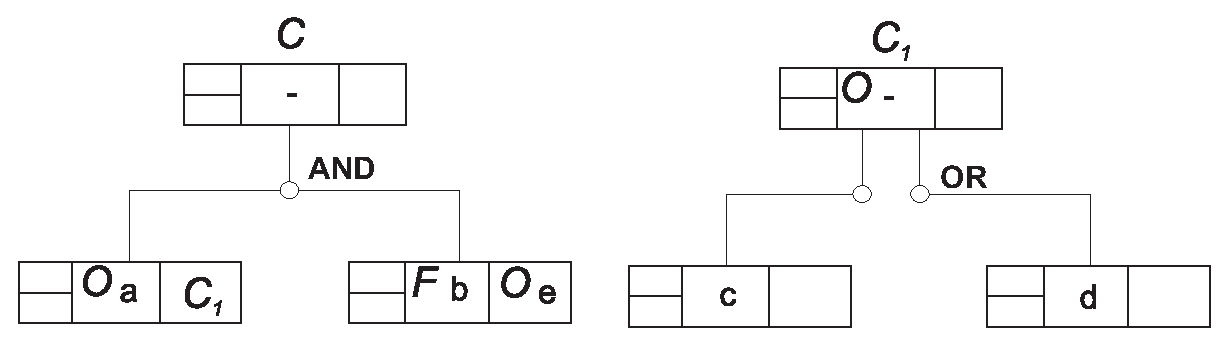
\includegraphics[width=10cm]{Figures/Reparations.eps}
%%\end{center}
%%  \caption{Reparations in \codiag}
%%  \label{Reparations}
%%\end{figure}
%%
%%At this point we can see clearly the difference between having a composition of obligations over atomic actions and having an obligation over a compound action. While the former allows us to specify a different reparation for each one of the atomic actions we are obliged to do, the latter only allows us to specify one reparation for the compound action that is under the obligation operator. For the first case, we can consider the diagrams we have in Figure \ref{CompoundNorms}, where it is possible to specify a different reparation in each one of the leaf clauses of the diagrams. For the second case, we can imagine having the diagrams shown in Figure \ref{ObligationCompoundActions}, where we can only specify reparations in the no leaf clauses where we have the obligations, covering these reparations the whole composition of actions.
%%
%%\begin{figure}
%%\begin{center}
%%  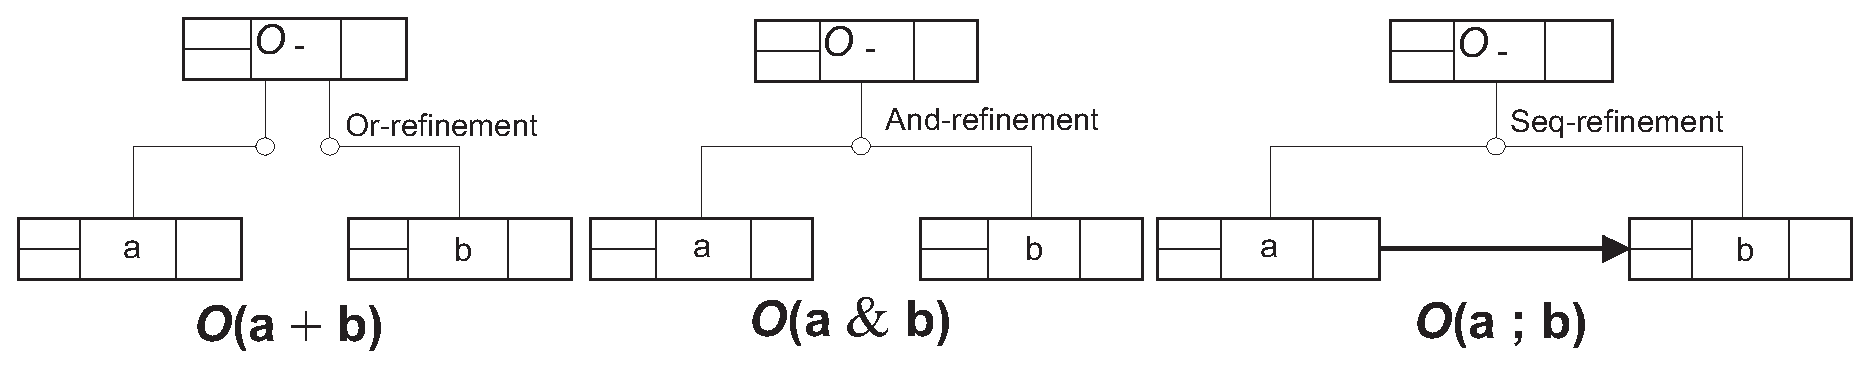
\includegraphics[width=12cm]{Figures/ObligationCompoundActions.eps}
%%\end{center}
%%  \caption{Obligations over compound actions}
%%  \label{ObligationCompoundActions}
%%\end{figure}
%%
%%This difference is a bit trickier if we consider prohibitions or permissions, because it not only concerns to the specification of reparations \cite{Pace2009}. For example, given two atomic actions \textit{a} and \textit{b}, the meaning of prohibiting the sequence of these two actions, written as \textit{F}(a$.$b), is different from the meaning of prohibiting action \textit{a}, and next prohibiting action \textit{b}, written as \textit{F}(a)$.$\textit{F}(b). In the first case, the sequence of actions starting with \textit{a} and continuing with any action different from \textit{b} is allowed, while in the second case any sequence of actions starting with \textit{a} is forbidden. In Figure \ref{ProhibitionActions} we can see how both cases are represented in our \codiag. Similar distinctions appear when we consider permissions instead of prohibitions.
%%
%%\begin{figure}
%%\begin{center}
%%  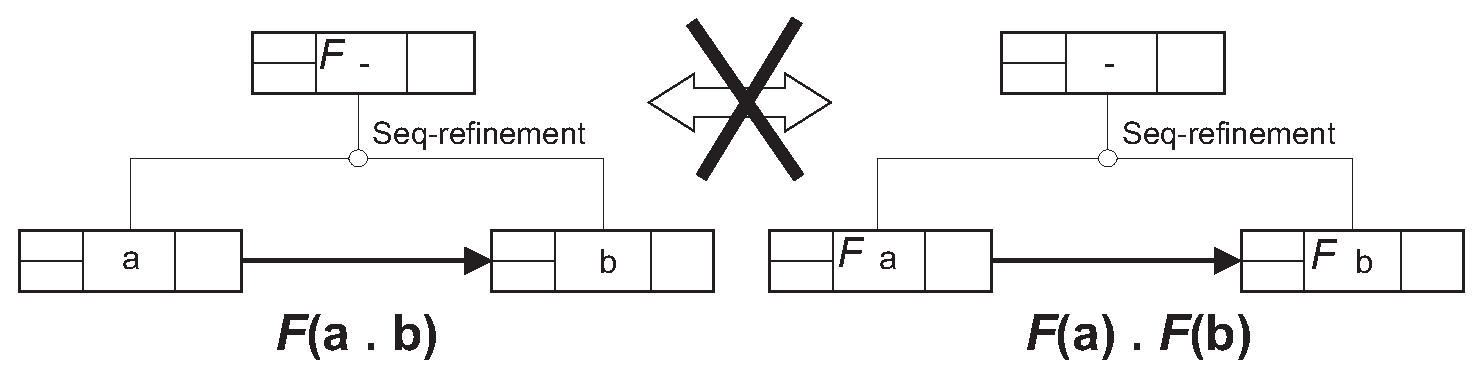
\includegraphics[width=12cm]{Figures/ProhibitionActions.eps}
%%\end{center}
%%  \caption{Prohibition of a sequence \textit{vs.} sequence of prohibitions}
%%  \label{ProhibitionActions}
%%\end{figure}
%%
%%\paragraph{\textbf{Guard g}} This element of a box is a \textit{boolean expression} that evaluates some information provided by the clause specification, telling us under which conditions the clause must be taken into account. For example, in a car insurance contract we can have a clause that is only applied to people who are under the age of 21. In that case, we must include in the box modelling this clause a guard similar to \textbf{age $<$ 21}, where \textbf{age} is a variable containing how old the client is and \textbf{21} is an integer value.
%%
%%Basically, a guard is a set of expressions that evaluate to a boolean (\textit{true} or \textit{false}) combined by means of conjunctions (\textit{and}), disjunctions (\textit{or}), and negations (\textit{not}). These expressions can include constant values, variables, and equality and inequality operators (\textit{$==$},\textit{$!=$},\textit{$<$},\textit{$>$}, \ldots). 
%%
%%The interpretation of these guards within the different kinds of refinement is the following:
%%
%%\begin{itemize}
%%
%%\item When the guard condition corresponding to a subclause of an \textbf{AND-refinement} or a \textbf{SEQ-refinement} evaluates to \textit{false}, the subclause is trivially satisfied, so we only must check the subclauses with a \textit{true} guard (or without guard).
%%
%%\item When the guard condition corresponding to a subclause of an \textbf{OR-refinement} evaluates to \textit{false}, we cannot satisfy that subclause in order to satisfy the parent clause, so it is necessary to satisfy one of the other subclauses with a \textit{true} guard (or without guard).
%%
%%\end{itemize}
%%
%%\paragraph{\textbf{Time restriction tr}} This element allows us to include timing aspects in the boxes of our diagram. In this way, we can associate deadlines, timeouts, etc. to the clauses of our contract. These real-time aspects are expressed in the boxes of our diagram by means of \textit{intervals} within \textbf{tr}. These intervals indicate the period of time in which the clauses must be satisfied.
%%
%%The time restrictions can be specified in two different ways within the boxes: we can specify the \textit{dates} binding the beginning and the end of the time frame corresponding to the clause (\textit{absolute time}), or we can specify a deadline saying the number of \textit{time units} that can elapse before the clause is satisfied from the moment at which another clause is satisfied or from the moment at which the contract comes into effect (\textit{relative time}). 
%%
%%For example, in the case of absolute time, we can model a contract stating that a clause must be satisfied in the \textbf{first five days of October}, as shown on the top of Figure \ref{TimeIntervals} (a). In the case of relative time, a contract can state that a clause must be satisfied not later than \textbf{five days after satisfying other clause}, as shown on the bottom of Figure \ref{TimeIntervals} (b), where \textit{SubClause3} must be satisfied before five days after satisfying \textit{SubClause1} (abridged as \textit{S.C.1}).
%%
%%\begin{figure}
%%\begin{center}
%%  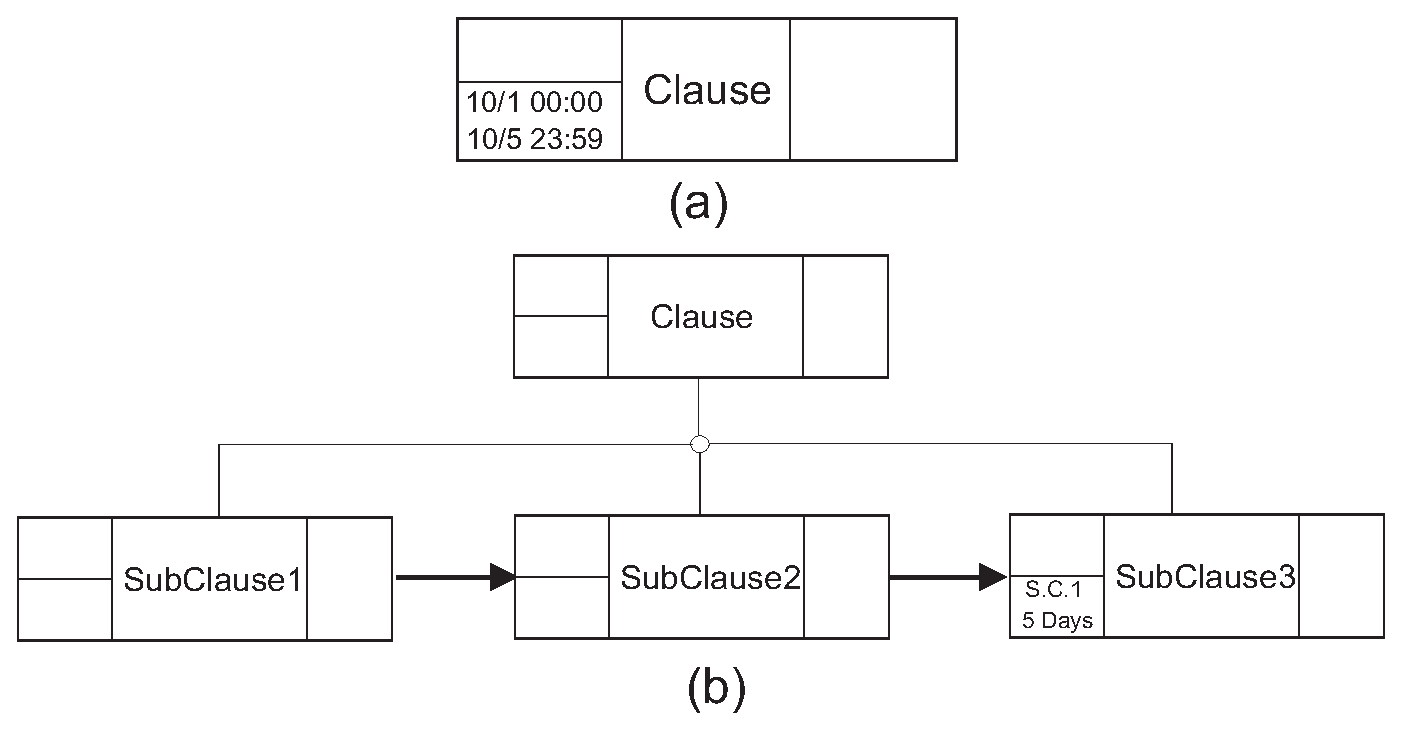
\includegraphics[width=12cm]{Figures/TimeIntervals.eps}
%%\end{center}
%%  \caption{\codiag\ with time restrictions}
%%  \label{TimeIntervals}
%%\end{figure}
%%
%%When we have a time restriction specified in a clause of the diagram that is refined into subclauses, this restriction affects all the subclauses. That is, all the subclauses necessary to satisfy the parent clause must be satisfied in the time frame specified in this parent clause. Otherwise, the parent clause is considered unfulfilled.
%%
%%%%Evaluation of the model%%
%%\subsection{Evaluation of the Model}
%%
%%%%Qualitative evaluation%%
%%In this subsection we present a qualitative evaluation of the visual model proposed for the description of electronic contracts. For this evaluation we discuss how the model fits some of the most important principles for designing effective visual notations defined in \cite{Moody2009}.
%%
%%First, the principle of \textit{semiotic clarity} is accomplished by the model, as there is only one graphical structure corresponding to each semantic concept and vice versa.
%%
%%Second, the principle of \textit{perceptual discriminability} is taken into account to differentiate between refinements, having each kind of refinement a clearly distinct shape and using the text with the name of the refinement to complement the graphics (principle of \textit{dual coding}).
%%
%%We also have that the number of different graphical symbols in the model is under the upper limit of six categories for graphics complexity, so the principle of \textit{graphic economy} is accomplished.
%%
%%Finally, the principle of \textit{complexity management} is covered by the modularization of the diagrams, where different modules can be integrated by means of a same box appearing in several diagrams (principle of \textit{cognitive integration}).
%%
%%%%%Model syntax%%%
%%\section{\codiag\ Syntax}\label{Syntax}
%%\markright{~\ref{Syntax} \codiag\ Syntax}
%%
%%\bdfn\label{defCOSyntax} (C-O Diagrams Syntax) \\
%%
%%We consider a finite set of real-valued variables $\mathcal{C}$ standing for clocks, a finite set of non-negative integer-valued variables $\mathcal{V}$, a finite alphabet $\Sigma$ for atomic actions, a finite set of identifiers $\mathcal{A}$ for agents, and another finite set of identifiers $\mathcal{N}$ for names. The Greek letter $\epsilon$ means that an expression is not given, i.e., it is empty.
%%
%%We use $C$ to denote the contract modelled by a \textit{C-O Diagram}. The diagram is defined by the following EBNF grammar:
%%
%%\begin{center}
%%\begin{tabular}{rcl}
%%    $C$ & $:=$ &  \begin{array}[t]{l}
%%						      (agent,name,g,tr,O(C_2),R) \,|\,
%%									(agent,name,g,tr,P(C_2),\epsilon) \,|\,	      
%%						      \end{array} \\    
%%		&  &  \begin{array}[t]{l}		      
%%		      (agent,name,g,tr,F(C_2),R) \,|\,
%%					(\epsilon,name,g,tr,C_1,\epsilon)
%%		      \end{array} \\		
%%    $C_1$ & $:=$ &  \begin{array}[t]{l}
%%								      C \,(And \; C)^+\,|\,
%%								      C \,(Or \; C)^+\,|\,
%%								      C \,(Seq \; C)^+
%%								      \end{array} \\
%%		$C_2$ & $:=$ &  \begin{array}[t]{l}
%%											a \,|\,
%%								      C_3 \,(And \; C_3)^+\,|\,
%%								      C_3 \,(Or \; C_3)^+\,|\,
%%								      C_3 \,(Seq \; C_3)^+
%%								      \end{array} \\
%%    $C_3$ & $:=$ &  \begin{array}[t]{l}
%%								      (\epsilon,name,\epsilon,\epsilon,C_2,\epsilon)								      
%%								      \end{array} \\
%%		$R$ & $:=$ &  \begin{array}[t]{l}
%%						      C \,|\,
%%						      \epsilon
%%						      \end{array} \\		
%%\end{tabular}
%%\end{center}
%%\noindent where $a \in \Sigma$, $agent \in \mathcal{A}$ and $name \in \mathcal{N}$. Guard $g$ is $\epsilon$ or a conjunctive formula of atomic constraints of the form: $v \sim n$ or $v - w \sim n$, for $v,w\in \mathcal{V}$, $\sim \in \{\, \leq, <, =, >, \geq \, \}$ and $n \in \nat$, whereas timed restriction $tr$ is $\epsilon$ or a conjunctive formula of atomic constraints of the form: $x \sim n$ or $x -y \sim n$, for $x,y \in \mathcal{C}$, $\sim \in \{\, \leq, <, =, >, \geq \, \}$ and $n \in \nat$. $O$, $P$ and $F$ are the deontic operators corresponding to obligation, permission and prohibition, respectively, where $O(C_2)$ states the obligation of performing $C_2$, $F(C_2)$ states prohibition of performing $C_2$, and $P(C_2)$ states the permission of performing $C_2$. $And$, $Or$ and $Seq$ are the operators corresponding to the refinements we have in \codiag, AND-refinement, OR-refinement and SEQ-refinement, respectively.
%%
%%\edfn
%%
%%The most simple contract we can have in \codiag\ is that composed of only one box including the elements $agent$ and $name$. Optionally, we can specify a guard $g$ and a time restriction $tr$. We also have a deontic operator ($O$, $P$ or $F$) applied over an atomic action $a$, and in the case of obligations and prohibitions it is possible to specify another contract $C$ as a reparation. E.g., $C:=(Buyer,Example1,\epsilon,\epsilon,O(pay),C^\prime)$ (Figure \ref{GrammarExamples}, on the bottom left) is a very simple contract specifying for a buyer the obligation of paying, otherwise contract $C^\prime$ comes into effect.
%%
%%We use $C_1$ to define a more complex contract where we combine different deontic norms by means of any of the different refinements we have in \codiag. In the box where we have the refinement into $C_1$ we cannot specify an agent nor a reparation because these elements are always related to a single deontic norm, but we still can specify a guard $g$ and a time restriction $tr$ that affect all the deontic norms we combine. E.g., $C:=(\epsilon,Example2,\epsilon,x<5,C^\prime \, Or \, C^{\prime\prime},\epsilon)$ (Figure \ref{GrammarExamples}, on the top left) is a composed contract specifying that contract $C^\prime$ or contract $C^{\prime\prime}$ must be satisfied in order to satisfy $C$ within 5 time units.
%%
%%Once we write a deontic operator in a box of our diagram, we have two possibilities as we can see in the specification of $C_2$: we can just write a simple action $a$ in the box, being the deontic operator applied only over it, or we can refine this box in order to apply the deontic operator over a compound action. In this case we have that the subboxes ($C_3$) cannot define a new deontic operator as it has already been defined in the parent box (affecting all the subboxes). Then, these subboxes cannot specify an agent nor a reparation. For example, $C:=(Buyer,Example3,\epsilon,\epsilon,O(C^\prime \, Or \, C^{\prime\prime}),\epsilon)$, where we have that $C^\prime:=(\epsilon,Option1,\epsilon,\epsilon,pay\_cash,\epsilon)$ and $C^{\prime\prime}:=(\epsilon,Option2,\epsilon,\epsilon,pay\_card,\epsilon)$ (Figure \ref{GrammarExamples}, on the right), is a contract specifying for a buyer the obligation of paying by cash or by credit card.
%%
%%\begin{figure}
%%\begin{center}
%%  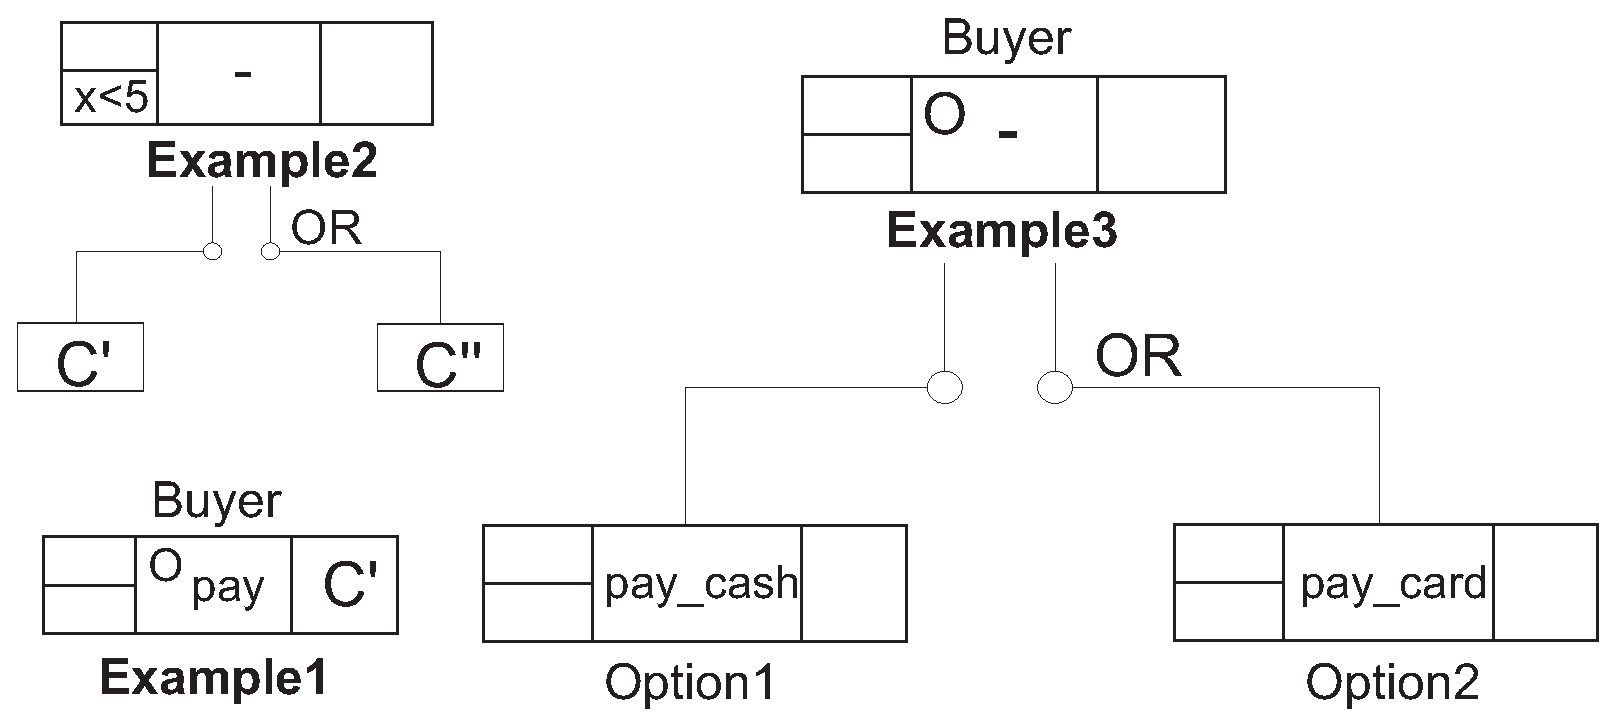
\includegraphics[width=9cm]{Figures/GrammarExamples.eps}
%%\end{center}  
%%  \caption{Syntax examples}
%%  \label{GrammarExamples}
%%\end{figure}
%%
%%%%%Model semantics%%%
%%\section{\codiag\ Semantics}\label{Semantics}
%%\markright{~\ref{Semantics} \codiag\ Semantics}
%%
%%%%Timed automata extensions for the model%%
%%The \codiag\ semantics is defined by means of a transformation into an NTA, adding the definition of two orderings, $\prec_N$ and $\prec_E$, where:
%%
%%\begin{itemize}
%%
%%\item $\prec_N$ is a (strict, partial) ordering on N where $n \prec_N n'$ means that node $n$ is better than node $n'$.
%%
%%\item $\prec_E$ is a (strict, partial) ordering on E where $e \prec_N e'$ means that edge $e$ is better than edge $e'$.
%%
%%\end{itemize}
%%
%%We also add a \textbf{violation set} $V(n)$ associated to each node $n$ in $N$, that is the set of contractual norms that are violated in $n$.
%%
%%\bdfn\label{defVio} (Violation Set) \\
%%
%%Let us consider the set of contractual norms $\mathcal{CN}$ ranged over $cn$, $cn'$, \ldots\ standing for identifiers of norms. We write $n \not \models cn$ to express that norm $cn$ is violated in node $n$. Therefore, the violation set is defined as $V(n)=\{cn \, | \, cn \in \mathcal{CN}$ and  $n \not \models cn\}$.
%%
%%\edfn
%%
%%Another set called \textbf{satisfaction set} $S(n)$ is also associated to each node $n$ in $N$. This set is composed by the contractual obligations and prohibitions that have already been satisfied in $n$. 
%%
%%\bdfn\label{defSat} (Satisfaction Set) \\
%%
%%Let us consider the set of contractual obligations and prohibitions $\mathcal{COF}$ ranged over $cof$, $cof'$, \ldots\ standing for identifiers of obligations and prohibitions. We write $n \models cof$ to express that obligation or prohibition $cof$ has been satisfied in node $n$ (we consider a prohibition satisfied in node $n$ if it has not been violated and cannot be violated anymore). Hence, the satisfaction set is defined as $S(n)=\{cof \, | \, cof \in \mathcal{COF}$ and  $n \models cof\}$.
%%
%%\edfn
%%
%%Once these two sets have been defined, we can formally define the \textbf{ordering on nodes} $\prec_N$, by comparing the violation sets and the satisfaction sets of the nodes, and the \textbf{ordering on edges} $\prec_E$, by comparing the violation sets and the satisfaction sets of the target nodes of the edges.
%%
%%\bdfn\label{defOrdN} (Ordering on Nodes) \\
%%
%%A node $n_1$ is better than another node $n_2$ if the violation set of $n_1$ is a proper subset of the violation set of $n_2$ or, if the violation sets are the same, a node $n_1$ is better than another node $n_2$ if the satisfaction set of $n_1$ is a proper superset of the satisfaction set of $n_2$, that is, $n_1 \prec_N n_2$ iff $(V(n_1) \subset V(n_2))$ or $(V(n_1) = V(n_2)$ and $S(n_1) \supset S(n_2))$.
%%
%%\edfn
%%
%%\bdfn\label{defOrdE} (Ordering on Edges) \\
%%
%%An edge $e_1$ is better than another edge $e_2$ if the source node is the same in both cases but the violation set of the target node of $e_1$ is a proper subset of the violation set of the target node of $e_2$ or, if the violation sets are the same, an edge $e_1$ is better than another edge $e_2$ if the satisfaction set of the target node of $e_1$ is a proper superset of the satisfaction set of the target node of $e_2$. Considering $e_1=(n_1,g_1,a_1,s_1,r_1,n{_1}')$ and $e_2=(n_2,g_2,a_2,s_2,r_2,n{_2}')$, $e_1 \prec_E e_2$ iff $(n_1=n_2)$ and $(V(n{_1}') \subset V(n{_2}')$ or $(V(n{_1}') = V(n{_2}')$ and $S(n{_1}') \supset S(n{_2}')))$.
%%
%%\edfn
%%
%%Finally, another set called \textbf{permission set} $P(n)$ is associated to each node $n$ in $N$. This set influences neither the ordering on nodes nor the ordering on edges, it is used just to record the permissions in the contract that have been made effective.
%%
%%\bdfn\label{defPer} (Permission Set) \\
%%
%%Let us consider the set of contractual permissions $\mathcal{CP}$ ranged over $cp$, $cp'$,\ldots\ standing for identifiers of permissions. We write $n \models cp$ to express that permission $cp$ has already been made effective in node $n$. Then, the permission set is defined as $P(n)=\{cp \, | \, cp \in \mathcal{CP}$ and  $n \models cp\}$.
%%
%%\edfn
%%
%%Graphically, when we draw a timed automaton extended with these three sets, we write under each node $n$ between braces its violation set $V(n)$ on the left, its satisfaction set $S(n)$ on the centre and its permission set $P(n)$ on the right. In the initial node of the automata we build corresponding to \codiag\ these three sets are empty. By default, a node keep in these sets the same content of the previous node. Only in a few cases the content of these sets is modified (when an obligation or a prohibition is violated, an obligation or a prohibition is satisfied or a permission is made effective).
%%
%%%%Time issues%%
%%Concerning the \textbf{real-time restrictions} $tr$ specified in the contract, the two types of time restrictions we can have in \codiag\ must be translated in a different way for their inclusion into a timed automaton construction:
%%
%%\begin{itemize}
%%
%%\item A time restriction specified using \textbf{absolute time} must be specified in timed automata by rewriting the terms in which absolute time references occur. For that purpose we define a global clock $T \in \mathcal{C}$ that is never reset during the execution of the automata and, taking into account the moment at which the contract is enacted, we rewrite the absolute time references as deadlines involving clock $T$ and considering the smallest time unit needed in the contract. For example, let us consider a clause that must be satisfied between the \textit{5th of November} and the \textit{10th of November}, and that the contract containing this clause is enacted the \textit{31st of October}. If we suppose that \textit{days} is the smallest time unit used in the contract for the specification of real-time restrictions, the time restriction of this clause is written as $(T \geq 5) \, and \, (T \leq 10)$.
%%
%%\item A time restriction specified using \textbf{relative time} must be specified in timed automata by introducing an additional clock to register the amount of time that has elapsed since another clause has been satisfied, resetting the additional clock value when this happens and specifying the deadline using it. We call this clock $t_{name}$, where $name$ is the clause used as reference for the specification of the time restriction. Therefore, we define a set of additional clocks $C_{add}=\{t_{name} \, | \,  t_{name} \in \mathcal{C}\}$ including a clock for every clause that is used as reference in the time restriction of at least another clause. For example, let us consider a contract with a clause that must be satisfied between \textit{5} and \textit{10} days after another clause $name1$ has been satisfied. In this case we define an additional clock $t_{name1}$ that is reset to zero when clause $name1$ is satisfied ($t_{name1}:=0$) and the time restriction of the other clause is written as $(t_{name1} \geq 5) \, and \, (t_{name1} \leq 10)$.
%%
%%\end{itemize}
%%
%%As a result, the set of clocks of the timed automata would be $\mathcal{C} = \{T\} \cup C_{add}$. When we construct the timed automata corresponding to \codiag, we always consider $(x \geq t1) \, and \, (x \leq t2)$ as the interval corresponding to the time restriction $tr$ of the clause, where $x \in \mathcal{C}$ is the clock used for its specification ($x=T$ in the case of absolute time and $x=t_{name}$ in the case of relative time, being $name$ the clause used as reference), $t1 \in \nat$ is the beginning of the interval and $t2 \in \nat$ is the end of the interval ($t1 \leq t2$). If $tr$ does not define the lower bound of the interval we take $t1=0$, if $tr$ does not define the upper bound of the interval we take $t2=\infty$, and if $tr = \epsilon$ we take $t1=0$, $t2=\infty$ and $x=T$.
%%
%%%%Timed automata construction rules%%
%%Once we have given these extensions of the definition of timed automata and we have explained how the different kinds of time restriction can be expressed, considering all the different elements we can specify in a \textit{C-O Diagram}, we can define the transformation of the diagrams into timed automata by induction using several transformation rules.
%%
%%\bdfn\label{defTR} (\codiag\ Transformation Rules: Part I)\\
%%
%%{\renewcommand{\labelenumi}{(\arabic{enumi})}
%%\begin{enumerate}
%%
%%%1
%%\item An \textbf{atomic action} in a \textit{C-O Diagram}, that is, $(\epsilon,name,\epsilon,\epsilon,a,\epsilon)$ corresponds to the timed automaton $\mathcal{A}=(N_{\mathcal{A}}, n_{0_{\mathcal{A}}}, E_{\mathcal{A}}, I_{\mathcal{A}})$, where:
%%
%%\begin{itemize}
%%
%%\item $N_{\mathcal{A}}=\{a_{init},a_{end}\}$.
%%
%%\item $n_{0_{\mathcal{A}}}=a_{init}$.
%%
%%\item $E_{\mathcal{A}}=\{a_{init} \flechald{a}{} a_{end}\}$.
%%
%%\item $I_{\mathcal{A}}=\emptyset$.
%%
%%\end{itemize}
%%
%%The violation (\textbf{V}), satisfaction (\textbf{S}) and permission (\textbf{P}) sets are not modified, so $V(a_{init})=V(a_{end})$, $S(a_{init})=S(a_{end})$ and $P(a_{init})=P(a_{end})$. This timed automaton can be seen in Figure \ref{automaton_A1}.
%%
%%\begin{figure}
%%\begin{center}
%%  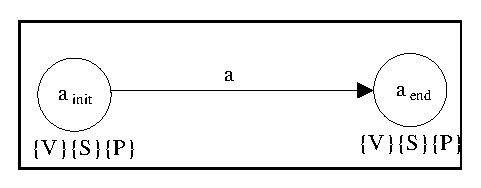
\includegraphics[width=5cm]{Figures/automaton_a1.eps}
%%\end{center}
%%  \caption{Automaton corresponding to a \textbf{simple action} $a$}
%%  \label{automaton_A1}
%%\end{figure}
%%
%%\separ
%%
%%%2
%%\item A \textbf{compound action} in a \textit{C-O Diagram} where an \textbf{AND-refinement} is used to compose actions, that is, $(\epsilon,name,\epsilon,\epsilon,C_1 \, And \, C_2 \, And \ldots And \, C_n,\epsilon)$ corresponds to the cartesian product of the automata corresponding to each one of the subcontracts. Let us consider $\mathcal{A}, \mathcal{B}, \ldots, \mathcal{Z}$ the automata corresponding to the subcontracts $C_1, C_2, \ldots, C_n$ (the actions specified in these subcontracts can be atomic actions or other compound actions). The resulting automaton $\mathcal{AND}$ corresponds to the cartesian product of these automata, that is, $\mathcal{AND} = \mathcal{A} \times \mathcal{B} \times \ldots \times \mathcal{Z}$. Again, the violation (\textbf{V}), satisfaction (\textbf{S}) and permission (\textbf{P}) sets are not modified, so they are the same in all the nodes. This composition of timed automata is shown graphically in Figure \ref{automaton_A2}.
%%
%%\begin{figure}
%%\begin{center}
%%  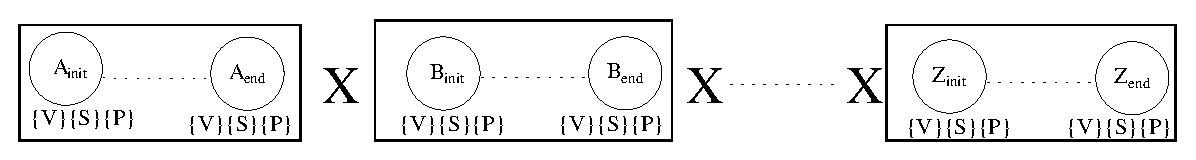
\includegraphics[width=12cm]{Figures/automaton_a2.eps}
%%\end{center}
%%  \caption{Automaton corresponding to a \textbf{compound action} (AND-refinement)}
%%  \label{automaton_A2}
%%\end{figure}
%%
%%\separ
%%
%%%3
%%\item A \textbf{compound action} in a \textit{C-O Diagram} where an \textbf{OR-refinement} is used to compose actions, that is, $(\epsilon,name,\epsilon,\epsilon,C_1 \, Or \, C_2 \, Or \ldots Or \, C_n,\epsilon)$ corresponds to a new automaton in which the automata corresponding to each one of the subcontracts is considered as an alternative. Let us consider $\mathcal{A}, \mathcal{B}, \ldots, \mathcal{Z}$ the automata corresponding to the subcontracts $C_1, C_2, \ldots, C_n$ (the actions specified in these subcontracts can be atomic actions or other compound actions). The resulting automaton $\mathcal{OR}$ preserves the structure of the automata we are composing but adding a new initial node $OR_{init}$ and connecting this node by means of urgent edges performing no action to the initial nodes of $\mathcal{A}, \mathcal{B}, \ldots, \mathcal{Z}$ ($A_{init}, B_{init}, \ldots, Z_{init}$). It is also added a new ending node $OR_{end}$ and urgent edges performing no action from the ending nodes of $\mathcal{A}, \mathcal{B}, \ldots, \mathcal{Z}$ ($A_{end}, B_{end}, \ldots, Z_{end}$) to this new ending node. Let $\mathcal{A}=(N_{\mathcal{A}}, n_{0_{\mathcal{A}}}, E_{\mathcal{A}}, I_{\mathcal{A}}), \mathcal{B}=(N_{\mathcal{B}}, n_{0_{\mathcal{B}}}, E_{\mathcal{B}}, I_{\mathcal{B}}), \ldots, \mathcal{Z}=(N_{\mathcal{Z}}, n_{0_{\mathcal{Z}}}, E_{\mathcal{Z}}, I_{\mathcal{Z}})$. The resulting automaton is therefore $\mathcal{OR}=(N_{\mathcal{OR}}, n_{0_{\mathcal{OR}}}, E_{\mathcal{OR}}, I_{\mathcal{OR}})$, where:
%%
%%\begin{itemize}
%%
%%\item $N_{\mathcal{OR}}=N_{\mathcal{A}} \cup N_{\mathcal{B}} \cup \ldots \cup N_{\mathcal{Z}}\cup \{OR_{init},OR_{end}\}$.
%%
%%\item $n_{0_{\mathcal{OR}}}=OR_{init}$.
%%
%%\item $E_{\mathcal{OR}}=E_{\mathcal{A}} \cup E_{\mathcal{B}} \cup \ldots \cup E_{\mathcal{Z}} \cup \{OR_{init} \flechalu{}{} A_{init}, OR_{init} \flechalu{}{} B_{init}, \ldots,$\\
%%$OR_{init} \flechalu{}{} Z_{init}\} \cup \{A_{end} \flechalu{}{} OR_{end}, B_{end} \flechalu{}{} OR_{end}, \ldots,$\\
%%$Z_{end} \flechalu{}{} OR_{end}\}$.
%%
%%\item $I_{\mathcal{OR}}=I_{\mathcal{A}} \cup I_{\mathcal{B}} \cup \ldots \cup I_{\mathcal{Z}}$.
%%
%%\end{itemize}
%%
%%The violation (\textbf{V}), satisfaction (\textbf{S}) and permission (\textbf{P}) sets are not modified, so they are the same in all the nodes. This composition of timed automata is shown graphically in Figure \ref{automaton_A3}.
%%
%%\begin{figure}
%%\begin{center}
%%  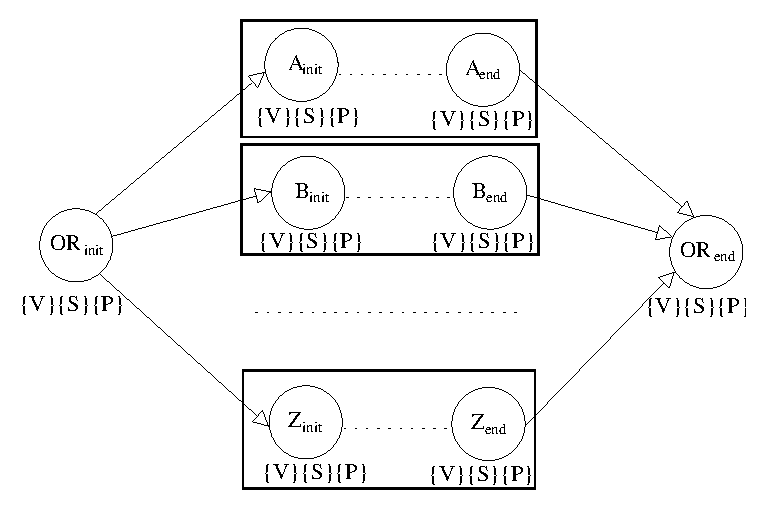
\includegraphics[width=7cm]{Figures/automaton_a3.eps}
%%\end{center}
%%  \caption{Automaton corresponding to a \textbf{compound action} (OR-refinement)}
%%  \label{automaton_A3}
%%\end{figure}
%%
%%\separ
%%
%%%4
%%\item A \textbf{compound action} in a \textit{C-O Diagram} where a \textbf{SEQ-refinement} is used to compose actions, that is, $(\epsilon,name,\epsilon,\epsilon,C_1 \, Seq \, C_2 \, Seq \ldots Seq \, C_n,\epsilon)$ corresponds to a new automaton in which the automata corresponding to each one of the subcontracts are connected in sequence. Let us consider $\mathcal{A}, \mathcal{B}, \ldots, \mathcal{Z}$ the automata corresponding to the subcontracts $C_1, C_2, \ldots, C_n$ (the actions specified in these subcontracts can be atomic actions or other compound actions). The resulting automaton $\mathcal{SEQ}$ preserves the structure of the automata we are composing, adding no extra nodes. We only connect with an urgent edge performing no action the ending node of each automaton in the sequence ($A_{end}, B_{end}, \ldots, Y_{end}$) with the initial node of the next automaton in the sequence ($B_{init}, C_{init}, \ldots, Z_{init}$). This rule is not applied in the cases of $A_{init}$ (as there is not previous ending node to connect) and $Z_{end}$ (as there is not following initial node to connect). Let $\mathcal{A}=(N_{\mathcal{A}}, n_{0_{\mathcal{A}}}, E_{\mathcal{A}}, I_{\mathcal{A}}), \mathcal{B}=(N_{\mathcal{B}}, n_{0_{\mathcal{B}}}, E_{\mathcal{B}}, I_{\mathcal{B}}), \ldots, \mathcal{Z}=(N_{\mathcal{Z}}, n_{0_{\mathcal{Z}}}, E_{\mathcal{Z}}, I_{\mathcal{Z}})$. The resulting automaton is therefore $\mathcal{SEQ}=(N_{\mathcal{SEQ}}, n_{0_{\mathcal{SEQ}}}, E_{\mathcal{SEQ}}, I_{\mathcal{SEQ}})$, where:
%%
%%\begin{itemize}
%%
%%\item $N_{\mathcal{SEQ}}=N_{\mathcal{A}} \cup N_{\mathcal{B}} \cup \ldots \cup N_{\mathcal{Z}}$.
%%
%%\item $n_{0_{\mathcal{SEQ}}}=A_{init}$.
%%
%%\item $E_{\mathcal{SEQ}}=E_{\mathcal{A}} \cup E_{\mathcal{B}} \cup \ldots \cup E_{\mathcal{Z}} \cup \{A_{end} \flechalu{}{} B_{init}, B_{end} \flechalu{}{} C_{init}, \ldots,$\\
%%$Y_{end} \flechalu{}{} Z_{init}\}$.
%%
%%\item $I_{\mathcal{SEQ}}=I_{\mathcal{A}} \cup I_{\mathcal{B}} \cup \ldots \cup I_{\mathcal{Z}}$.
%%
%%\end{itemize}
%%
%%Again, the violation (\textbf{V}), satisfaction (\textbf{S}) and permission (\textbf{P}) sets are not modified, so they are the same in all the nodes. This composition of timed automata is shown graphically in Figure \ref{automaton_A4}.
%%
%%\begin{figure}
%%\begin{center}
%%  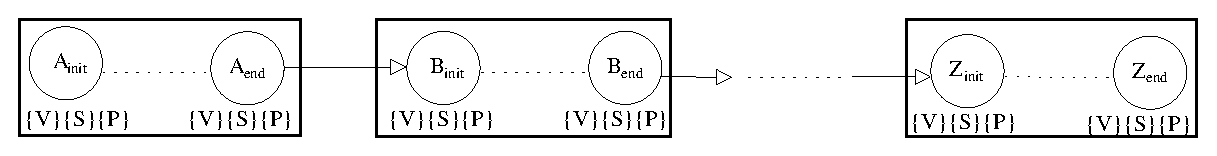
\includegraphics[width=12cm]{Figures/automaton_a4.eps}
%%\end{center}
%%  \caption{Automaton corresponding to a \textbf{compound action} (SEQ-refinement)}
%%  \label{automaton_A4}
%%\end{figure}
%%
%%\end{enumerate}
%%
%%}
%%
%%\edfnt
%%
%%Until now, we have seen how the automata corresponding to the different actions (atomic or compound) specified in a \textit{C-O Diagram} are constructed and we have seen that these translations do not modify the content of any of the sets (violation, satisfaction or prohibition). Next, we define the transformation rules specifying how these ``action'' automata are modified when we apply a deontic norm (obligation, permission or prohibition) over the actions in the \textit{C-O Diagram}.
%%
%%\setcounter{definition}{13}
%%\bdfn (\codiag\ Transformation Rules: Part II)\\
%%
%%{\renewcommand{\labelenumi}{(\arabic{enumi})}
%%\begin{enumerate}
%%
%%\setcounter{enumi}{4}
%%
%%%5
%%\item The application of an \textbf{obligation} over an action in a \textit{C-O Diagram}, that is, $(agent,name,g,tr,O(C),R)$ corresponds to an automaton where the obligation of performing the action specified in the subcontract $C$ can be skipped, fulfilled or violated. Let us consider $\mathcal{A}=(N_{\mathcal{A}}, n_{0_{\mathcal{A}}}, E_{\mathcal{A}}, I_{\mathcal{A}})$ the automaton corresponding to $C$, being $A_{init}$ the initial node and $A_{end}$ the ending node. The resulting automaton $\mathcal{O(A)}$ preserves the structure of the automaton $\mathcal{A}$ but adding a new ending node $A_{time}$ including the obligation over the action in its violation set and, if guard condition $g \neq \epsilon$, adding another ending node $A_{skip}$ where the violation, satisfaction and permission sets are not modified. We also include the obligation over the action in the satisfaction set of $A_{end}$. An invariant $x \leq t2 + 1$ is added to each node of $\mathcal{A}$ except $A_{end}$ and each edge performing one of the obliged actions in this automaton is guarded with $(x \geq t1) \, and \, (x \leq t2)$ and action performed by $agent$. New edges guarded with $x = t2 + 1$ and no action performed are added from each node of $\mathcal{A}$ except $A_{end}$ to the new node $A_{time}$ and, if guard condition $g \neq \epsilon$, an urgent edge from $A_{init}$ to $A_{skip}$ is also added guarded with the guard condition of the clause negated ($\neg g$). Finally, if $t_{name} \in \mathcal{C}$, all the edges reaching $A_{end}$ reset $t_{name}$ to zero.
%%
%%Considering the more complex case, where $g \neq \epsilon$ and $t_{name} \in \mathcal{C}$, and having that $g_1 \equiv (x \geq t1) \, and \, (x \leq t2)$ and $g_2 \equiv x = t2 + 1$, the resulting automaton is therefore $\mathcal{O(A)}=(N_{\mathcal{O(A)}}, n_{0_{\mathcal{O(A)}}}, E_{\mathcal{O(A)}}, I_{\mathcal{O(A)}})$, where:
%%
%%\begin{itemize}
%%
%%\item $N_{\mathcal{O(A)}}=N_{\mathcal{A}} \cup \{A_{time},A_{skip}\}$.
%%
%%\item $n_{0_{\mathcal{O(A)}}}=A_{init}$.
%%
%%\item $E_{\mathcal{O(A)}}=\{n \xrightarrow[]{g_1,agent(a)} n' \, | \, n \flechald{a}{} n' \in E_{\mathcal{A}}$ and $n' \neq A_{end}\} \cup$\\
%%$\{n \xrightarrow[]{g_1,agent(a),t_{name}} n' \, | \, n \flechald{a}{} n' \in E_{\mathcal{A}}$ and $n'=A_{end}\} \cup \{n \flechald{g_2}{} A_{time} \, | \, n \in N_{\mathcal{A}}-\{A_{end}\}\} \cup \{A_{init} \flechalu{\neg g}{} A_{skip}\}$.
%%
%%\item $I_{\mathcal{O(A)}}=I_{\mathcal{A}} \cup \{I(n) \equiv x \leq t2 + 1 \, | \, n \in N_{\mathcal{A}}-\{A_{end}\}\}$.
%%
%%\end{itemize}
%%
%%The resulting timed automaton is shown graphically in Figure \ref{automaton_A5}, where we consider $a$ one of the atomic actions included in the subcontract $C$.
%%
%%\begin{figure}
%%\begin{center}
%%  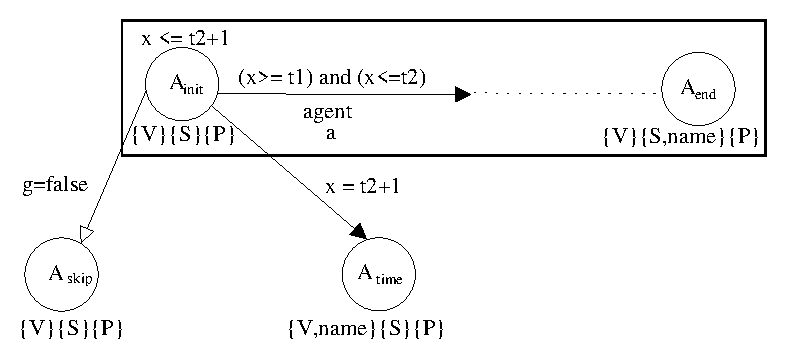
\includegraphics[width=8cm]{Figures/automaton_a5.eps}
%%\end{center}
%%  \caption{Automaton corresponding to an \textbf{obligation} over an action}
%%  \label{automaton_A5}
%%\end{figure}
%%
%%\separ
%%
%%%6
%%\item The application of a \textbf{permission} over an action in a \textit{C-O Diagram}, that is, $(agent,name,g,tr,P(C),\epsilon)$ corresponds to an automaton where the permission of performing the action specified in the subcontract $C$ can be skipped, made effective or not made effective. Let us consider $\mathcal{A}=(N_{\mathcal{A}}, n_{0_{\mathcal{A}}}, E_{\mathcal{A}}, I_{\mathcal{A}})$ the automaton corresponding to $C$, being $A_{init}$ the initial node and $A_{end}$ the ending node. The resulting automaton $\mathcal{P(A)}$ preserves the structure of the automaton $\mathcal{A}$ but adding a new ending node $A_{time}$ where the violation, satisfaction and permission sets are not modified as permissions cannot be violated and, if guard condition $g \neq \epsilon$, adding another ending node $A_{skip}$ where these sets are not modified again. We also include the permission over the action in the permission set of $A_{end}$. An invariant $x \leq t2 + 1$ is added to each node of $\mathcal{A}$ except $A_{end}$ and each edge performing one of the permitted actions in this automaton is guarded with $(x \geq t1) \, and \, (x \leq t2)$ and action performed by $agent$. New edges guarded with $x = t2 + 1$ and no action performed are added from each node of $\mathcal{A}$ except $A_{end}$ to the new node $A_{time}$ and, if guard condition $g \neq \epsilon$, an urgent edge from $A_{init}$ to $A_{skip}$ is also added guarded with the guard condition of the clause negated ($\neg g$). Finally, if $t_{name} \in \mathcal{C}$, all the edges reaching $A_{end}$ reset $t_{name}$ to zero.
%%
%%Considering the more complex case, where $g \neq \epsilon$ and $t_{name} \in \mathcal{C}$, and having that $g_1 \equiv (x \geq t1) \, and \, (x \leq t2)$ and $g_2 \equiv x = t2 + 1$, the resulting automaton is therefore $\mathcal{P(A)}=(N_{\mathcal{P(A)}}, n_{0_{\mathcal{P(A)}}}, E_{\mathcal{P(A)}}, I_{\mathcal{P(A)}})$, where:
%%
%%\begin{itemize}
%%
%%\item $N_{\mathcal{P(A)}}=N_{\mathcal{A}} \cup \{A_{time},A_{skip}\}$.
%%
%%\item $n_{0_{\mathcal{P(A)}}}=A_{init}$.
%%
%%\item $E_{\mathcal{P(A)}}=\{n \xrightarrow[]{g_1,agent(a)} n' \, | \, n \flechald{a}{} n' \in E_{\mathcal{A}}$ and $n' \neq A_{end}\} \cup$\\
%%$\{n \xrightarrow[]{g_1,agent(a),t_{name}} n' \, | \, n \flechald{a}{} n' \in E_{\mathcal{A}}$ and $n'=A_{end}\} \cup \{n \flechald{g_2}{} A_{time} \, | \, n \in N_{\mathcal{A}}-\{A_{end}\}\} \cup \{A_{init} \flechalu{\neg g}{} A_{skip}\}$.
%%
%%\item $I_{\mathcal{P(A)}}=I_{\mathcal{A}} \cup \{I(n) \equiv x \leq t2 + 1 \, | \, n \in N_{\mathcal{A}}-\{A_{end}\}\}$.
%%
%%\end{itemize}
%%
%%The resulting timed automaton is shown graphically in Figure \ref{automaton_A6}, where we consider $a$ one of the atomic actions included in the subcontract $C$.
%%
%%\begin{figure}
%%\begin{center}
%%  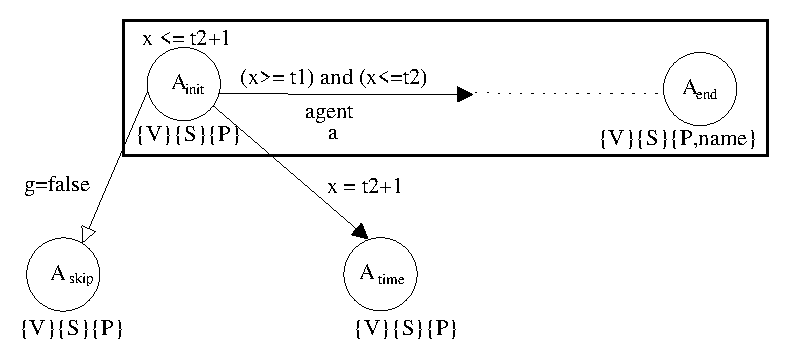
\includegraphics[width=8cm]{Figures/automaton_a6.eps}
%%\end{center}
%%  \caption{Automaton corresponding to a \textbf{permission} over an action}
%%  \label{automaton_A6}
%%\end{figure}
%%
%%\separ
%%
%%%7
%%\item The application of a \textbf{prohibition} over an action in a \textit{C-O Diagram}, that is, $(agent,name,g,tr,F(C),R)$ corresponds to an automaton where the prohibition of performing the action specified in the subcontract $C$ can be skipped, fulfilled or violated. Let us consider $\mathcal{A}=(N_{\mathcal{A}}, n_{0_{\mathcal{A}}}, E_{\mathcal{A}}, I_{\mathcal{A}})$ the automaton corresponding to $C$, being $A_{init}$ the initial node and $A_{end}$ the ending node. The resulting automaton $\mathcal{F(A)}$ preserves the structure of the automaton $\mathcal{A}$ but adding a new ending node $A_{time}$ including the prohibition over the action in its satisfaction set and, if guard condition $g \neq \epsilon$, adding another ending node $A_{skip}$ where the violation, satisfaction and permission sets are not modified. We also include the prohibition over the action in the violation set of $A_{end}$. An invariant $x \leq t2 + 1$ is added to each node of $\mathcal{A}$ except $A_{end}$ and each edge performing one of the prohibited actions in this automaton is guarded with $(x \geq t1) \, and \, (x \leq t2)$ and action performed by $agent$. New edges guarded with $x = t2 + 1$ and no action performed are added from each node of $\mathcal{A}$ except $A_{end}$ to the new node $A_{time}$ and, if guard condition $g \neq \epsilon$, an urgent edge from $A_{init}$ to $A_{skip}$ is also added guarded with the guard condition of the clause negated ($\neg g$). Finally, if $t_{name} \in \mathcal{C}$, all the edges reaching $A_{time}$ reset $t_{name}$ to zero.
%%
%%Considering the more complex case, where $g \neq \epsilon$ and $t_{name} \in \mathcal{C}$, and having that $g_1 \equiv (x \geq t1) \, and \, (x \leq t2)$ and $g_2 \equiv x = t2 + 1$, the resulting automaton is therefore $\mathcal{F(A)}=(N_{\mathcal{F(A)}}, n_{0_{\mathcal{F(A)}}}, E_{\mathcal{F(A)}}, I_{\mathcal{F(A)}})$, where:
%%
%%\begin{itemize}
%%
%%\item $N_{\mathcal{F(A)}}=N_{\mathcal{A}} \cup \{A_{time},A_{skip}\}$.
%%
%%\item $n_{0_{\mathcal{F(A)}}}=A_{init}$.
%%
%%\item $E_{\mathcal{F(A)}}=\{n \xrightarrow[]{g_1,agent(a)} n' \, | \, n \flechald{a}{} n' \in E_{\mathcal{A}}\} \cup \{n \xrightarrow[]{g_2,t_{name}} A_{time} \, | \, n \in N_{\mathcal{A}}-\{A_{end}\}\} \cup \{A_{init} \flechalu{\neg g}{} A_{skip}\}$.
%%
%%\item $I_{\mathcal{F(A)}}=I_{\mathcal{A}} \cup \{I(n) \equiv x \leq t2 + 1 \, | \, n \in N_{\mathcal{A}}-\{A_{end}\}\}$.
%%
%%\end{itemize}
%%
%%The resulting timed automaton is shown graphically in Figure \ref{automaton_A7}, where we consider $a$ one of the atomic actions included in the subcontract $C$.
%%
%%\begin{figure}
%%\begin{center}
%%  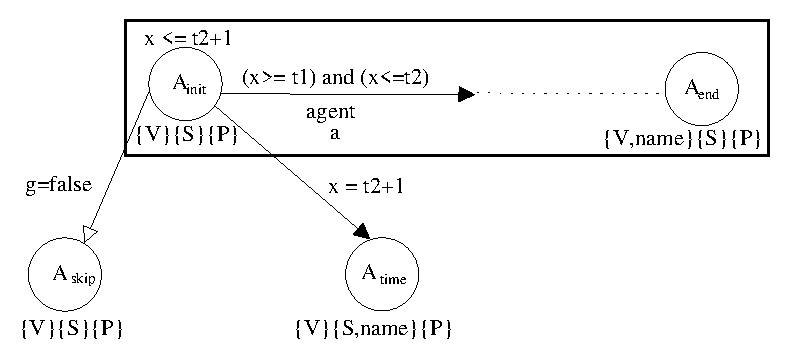
\includegraphics[width=8cm]{Figures/automaton_a7.eps}
%%\end{center}
%%  \caption{Automaton corresponding to a \textbf{prohibition} over an action}
%%  \label{automaton_A7}
%%\end{figure}
%%
%%\end{enumerate}
%%
%%}
%%
%%\edfnt
%%
%%We can see that the above constructions can include a reparation contract $R$ in the cases of obligation and prohibition. If this reparation is defined, we have to construct the automaton corresponding to the reparation contract and integrate this automaton as part of the automaton we have generated for the obligation or prohibition. This reparation contract remove the obliged or prohibited clause $name$ from the violation set of the corresponding automaton, as we can see in Figure \ref{automaton_AR}.
%%
%%\begin{figure}
%%\begin{center}
%%  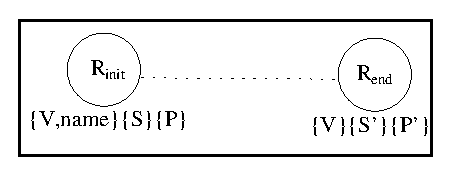
\includegraphics[width=5cm]{Figures/automaton_aR.eps}
%%\end{center}
%%  \caption{Automaton corresponding to a \textbf{reparation} $R$ of $name$}
%%  \label{automaton_AR}
%%\end{figure}
%%
%%\setcounter{definition}{13}
%%\bdfn (\codiag\ Transformation Rules: Part III)\\
%%
%%{\renewcommand{\labelenumi}{(\arabic{enumi})}
%%\begin{enumerate}
%%
%%\setcounter{enumi}{7}
%%
%%%8
%%\item An \textbf{obligation} in a \textit{C-O Diagram} specifying a contract \textbf{reparation} $R \neq \epsilon$ corresponds to the obligation automaton $\mathcal{O(A)}$ together with the reparation automaton $\mathcal{R}$, considering the node with $name$ in its violation set ($A_{time}$) as the initial node of the reparation automaton ($R_{init}$). In the ending node of the reparation automaton ($R_{end}$) $name$ is removed from the violation set, as the violation has been repaired. In this node we also have that the satisfaction set and the permission set are different from the ones we have in the initial node of the reparation because we have to include in the satisfaction set all the obligations and prohibitions satisfied in the reparation contract, and in the permission set all the permissions that have been made effective in the reparation contract. Let us consider $\mathcal{O(A)}=(N_{\mathcal{O(A)}}, n_{0_{\mathcal{O(A)}}}, E_{\mathcal{O(A)}}, I_{\mathcal{O(A)}})$  and $\mathcal{R}=(N_{\mathcal{R}}, n_{0_{\mathcal{R}}}, E_{\mathcal{R}}, I_{\mathcal{R}})$. The resulting automaton is therefore $\mathcal{O(A)_R}=(N_{\mathcal{O(A)_R}}, n_{0_{\mathcal{O(A)_R}}}, E_{\mathcal{O(A)_R}}, I_{\mathcal{O(A)_R}})$, where:
%%
%%\begin{itemize}
%%
%%\item $N_{\mathcal{O(A)_R}}=N_{\mathcal{O(A)}} \cup N_{\mathcal{R}}-\{R_{init}\}$.
%%
%%\item $n_{0_{\mathcal{O(A)_R}}}=A_{init}$.
%%
%%\item $E_{\mathcal{O(A)_R}}=E_{\mathcal{O(A)}} \cup \{n \flechald{g,a,r}{s} n' \, | \, n \flechald{g,a,r}{s} n' \in E_{\mathcal{R}}$ and $n \neq R_{init}\} \cup$\\
%%$\{A_{time} \flechald{g,a,r}{s} n' \, | \, n \flechald{g,a,r}{s} n' \in E_{\mathcal{R}}$ and $n=R_{init}\}$.
%%
%%\item $I_{\mathcal{O(A)_R}}=I_{\mathcal{O(A)}}-\{I(A_{time})\} \cup \{I(n)  \, | \, n \in  N_{\mathcal{R}}-\{R_{init}\}\} \cup \{I(A_{time}) \equiv $\\
%%$I(R_{init})\}$.
%%
%%\end{itemize}
%%
%%\separ
%%
%%%9
%%\item A \textbf{prohibition} in a \textit{C-O Diagram} specifying a contract \textbf{reparation} $R \neq \epsilon$ corresponds to the prohibition automaton $\mathcal{F(A)}$ together with the reparation automaton $\mathcal{R}$, considering the node with $name$ in its violation set ($A_{end}$) as the initial node of the reparation automaton ($R_{init}$). In the ending node of the reparation automaton ($R_{end}$) $name$ is removed from the violation set, as the violation has been repaired. In this node we also have that the satisfaction set and the permission set are different from the ones we have in the initial node of the reparation because we have to include in the satisfaction set all the obligations and prohibitions satisfied in the reparation contract, and in the permission set all the permissions that have been made effective in the reparation contract. Let us consider $\mathcal{F(A)}=(N_{\mathcal{F(A)}}, n_{0_{\mathcal{F(A)}}}, E_{\mathcal{F(A)}}, I_{\mathcal{F(A)}})$  and $\mathcal{R}=(N_{\mathcal{R}}, n_{0_{\mathcal{R}}}, E_{\mathcal{R}}, I_{\mathcal{R}})$. The resulting automaton is therefore $\mathcal{F(A)_R}=(N_{\mathcal{F(A)_R}}, n_{0_{\mathcal{F(A)_R}}}, E_{\mathcal{F(A)_R}}, I_{\mathcal{F(A)_R}})$, where:
%%
%%\begin{itemize}
%%
%%\item $N_{\mathcal{F(A)_R}}=N_{\mathcal{F(A)}} \cup N_{\mathcal{R}}-\{R_{init}\}$.
%%
%%\item $n_{0_{\mathcal{F(A)_R}}}=A_{init}$.
%%
%%\item $E_{\mathcal{F(A)_R}}=E_{\mathcal{F(A)}} \cup \{n \flechald{g,a,r}{s} n' \, | \, n \flechald{g,a,r}{s} n' \in E_{\mathcal{R}}$ and $n \neq R_{init}\} \cup$\\
%%$\{A_{end} \flechald{g,a,r}{s} n' \, | \, n \flechald{g,a,r}{s} n' \in E_{\mathcal{R}}$ and $n=R_{init}\}$.
%%
%%\item $I_{\mathcal{F(A)}}=I_{\mathcal{F(A)}}-\{I(A_{end})\} \cup \{I(n)  \, | \, n \in  N_{\mathcal{R}}-\{R_{init}\}\} \cup \{I(A_{end}) \equiv I(R_{init})\}$.
%%
%%\end{itemize}
%%
%%\end{enumerate}
%%
%%}
%%
%%\edfnt
%%
%%Finally, we have to define the rules about how the automata corresponding to different deontic norms are composed when we have a composition of deontic norms in our \textit{C-O Diagram}. To make this composition possible, first we need to have only one ending node in the automata corresponding to the different deontic norms. Therefore, we add a new ending node in these automata and urgent edges from the old ending nodes to this new node, as we show in Figure \ref{automaton_AF} for obligation, permission and prohibition. Notice that in the case of obligation and prohibition, if there is no reparation defined, the node violating the norm is a final node of the whole automaton construction where the contract is breached.
%%
%%\begin{figure}
%%\begin{center}
%%  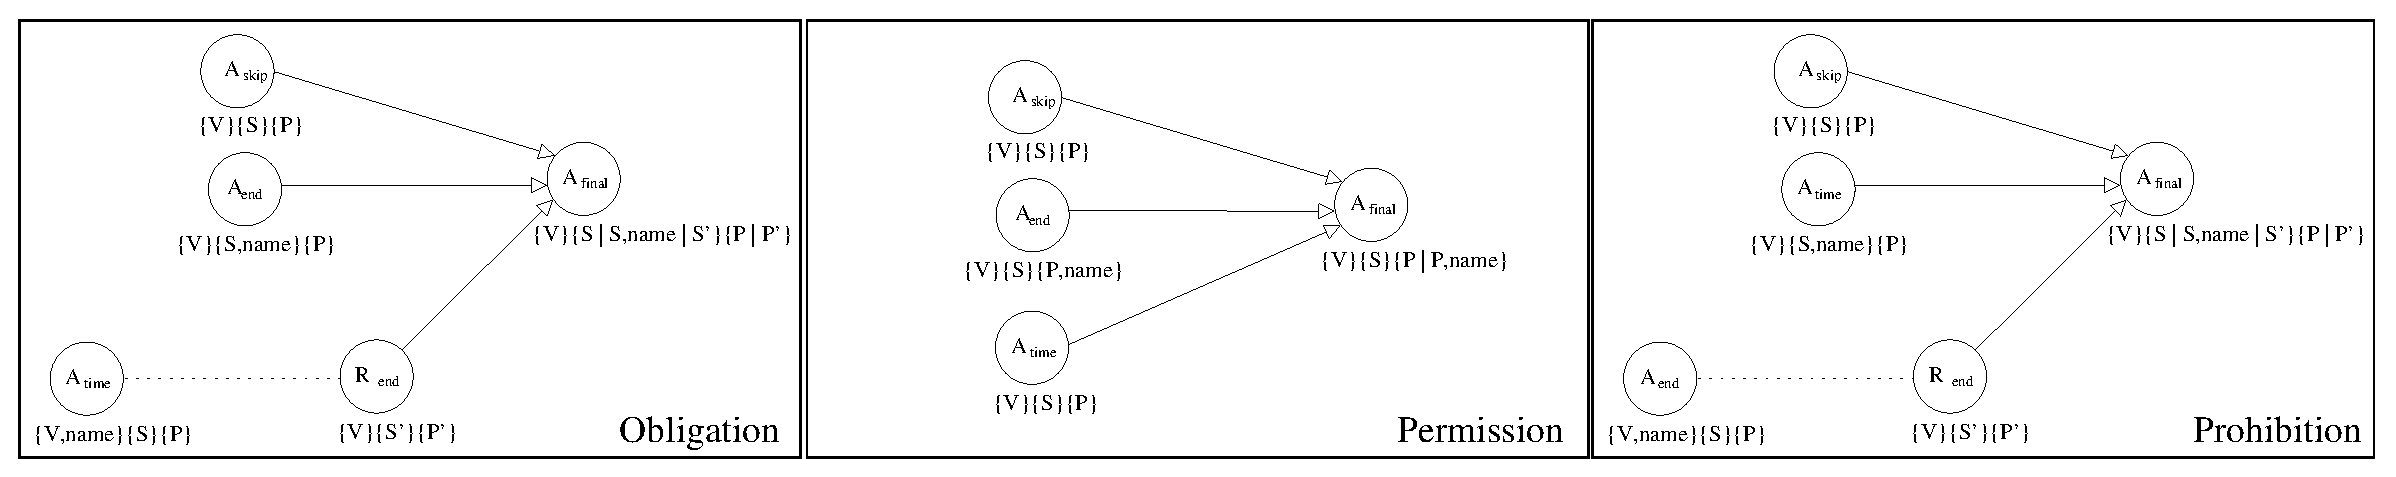
\includegraphics[width=12cm]{Figures/automaton_aF.eps}
%%\end{center}
%%  \caption{Addition of a unique final node in deontic norms automata}
%%  \label{automaton_AF}
%%\end{figure}
%%
%%\setcounter{definition}{13}
%%\bdfn (\codiag\ Transformation Rules: Part IV)\\
%%
%%{\renewcommand{\labelenumi}{(\arabic{enumi})}
%%\begin{enumerate}
%%
%%\setcounter{enumi}{9}
%%
%%%10
%%\item Let $\mathcal{O(A)_R}=(N_{\mathcal{O(A)_R}}, n_{0_{\mathcal{O(A)_R}}}, E_{\mathcal{O(A)_R}}, I_{\mathcal{O(A)_R}})$ be the automaton corresponding to an \textbf{obligation} in a \textit{C-O Diagram} specifying a \textbf{reparation} $R \neq \epsilon$. The corresponding automaton with only one ending node, that we call $A_{final}$ and preserves the violation, satisfaction and permission sets of the previous node, is $\mathcal{O(A)'_R}=(N_{\mathcal{O(A)'_R}}, n_{0_{\mathcal{O(A)'_R}}}, E_{\mathcal{O(A)'_R}}, I_{\mathcal{O(A)'_R}})$, where:
%%
%%\begin{itemize}
%%
%%\item $N_{\mathcal{O(A)'_R}}=N_{\mathcal{O(A)_R}} \cup \{A_{final}\}$.
%%
%%\item $n_{0_{\mathcal{O(A)'_R}}}=n_{0_{\mathcal{O(A)_R}}}$.
%%
%%\item $E_{\mathcal{O(A)'_R}}=E_{\mathcal{O(A)_R}} \cup \{A_{skip} \flechalu{}{} A_{final}\} \cup \{A_{end} \flechalu{}{} A_{final}\} \cup$\\
%%$ \{R_{end} \flechalu{}{} A_{final}\}$.
%%
%%\item $I_{\mathcal{O(A)'_R}}=I_{\mathcal{O(A)_R}}$.
%%
%%\end{itemize}
%%
%%\separ
%%
%%%11
%%\item Let $\mathcal{P(A)}=(N_{\mathcal{P(A)}}, n_{0_{\mathcal{P(A)}}}, E_{\mathcal{P(A)}}, I_{\mathcal{P(A)}})$ be the automaton corresponding to a \textbf{permission} in a \textit{C-O Diagram}. The corresponding automaton with only one ending node, that we call $A_{final}$ and preserves the violation, satisfaction and permission sets of the previous node, is $\mathcal{P(A)'}=(N_{\mathcal{P(A)'}}, n_{0_{\mathcal{P(A)'}}}, E_{\mathcal{P(A)'}}, I_{\mathcal{P(A)'}})$, where:
%%
%%\begin{itemize}
%%
%%\item $N_{\mathcal{P(A)'}}=N_{\mathcal{P(A)}} \cup \{A_{final}\}$.
%%
%%\item $n_{0_{\mathcal{P(A)'}}}=n_{0_{\mathcal{P(A)}}}$.
%%
%%\item $E_{\mathcal{P(A)'}}=E_{\mathcal{P(A)}} \cup \{A_{skip} \flechalu{}{} A_{final}\} \cup \{A_{end} \flechalu{}{} A_{final}\} \cup$\\
%%$ \{A_{time} \flechalu{}{} A_{final}\}$.
%%
%%\item $I_{\mathcal{P(A)'}}=I_{\mathcal{P(A)}}$.
%%
%%\end{itemize}
%%
%%\separ
%%
%%%12
%%\item Let $\mathcal{F(A)_R}=(N_{\mathcal{F(A)_R}}, n_{0_{\mathcal{F(A)_R}}}, E_{\mathcal{F(A)_R}}, I_{\mathcal{F(A)_R}})$ be the automaton corresponding to a \textbf{prohibition} in a \textit{C-O Diagram} specifying a \textbf{reparation} $R \neq \epsilon$. The corresponding automaton with only one ending node, that we call $A_{final}$ and preserves the violation, satisfaction and permission sets of the previous node, is $\mathcal{F(A)'_R}=(N_{\mathcal{F(A)'_R}}, n_{0_{\mathcal{F(A)'_R}}}, E_{\mathcal{F(A)'_R}}, I_{\mathcal{F(A)'_R}})$, where:
%%
%%\begin{itemize}
%%
%%\item $N_{\mathcal{F(A)'_R}}=N_{\mathcal{F(A)_R}} \cup \{A_{final}\}$.
%%
%%\item $n_{0_{\mathcal{F(A)'_R}}}=n_{0_{\mathcal{F(A)_R}}}$.
%%
%%\item $E_{\mathcal{F(A)'_R}}=E_{\mathcal{F(A)_R}} \cup \{A_{skip} \flechalu{}{} A_{final}\} \cup \{A_{time} \flechalu{}{} A_{final}\} \cup$\\
%%$ \{R_{end} \flechalu{}{} A_{final}\}$.
%%
%%\item $I_{\mathcal{F(A)'_R}}=I_{\mathcal{F(A)_R}}$.
%%
%%\end{itemize}
%%
%%\end{enumerate}
%%
%%}
%%
%%\edfnt
%%
%%Therefore, the composition of the automata corresponding to different deontic norms is defined by three additional transformation rules.
%%
%%\setcounter{definition}{13}
%%\bdfn (\codiag\ Transformation Rules: Part V)\\
%%
%%{\renewcommand{\labelenumi}{(\arabic{enumi})}
%%\begin{enumerate}
%%
%%\setcounter{enumi}{12}
%%
%%%13
%%\item If several norms are composed by an \textbf{AND-refinement}, that is, we have the diagram $(\epsilon,name,g,tr,C_1 \, And \, C_2 \, And \ldots And \, C_n,\epsilon)$, their composition corresponds to a network of automata in which we consider all the norms we are composing in parallel. Let us consider $\mathcal{C}_1, \mathcal{C}_2, \ldots, \mathcal{C}_n$ the automata corresponding to the norms we are composing. The resulting network of automata preserves the structure of the automata we are composing, adding to each one of them the additional nodes and edges necessary for synchronization (these nodes are called $C_{init}$ and $C_{final}$ in the first automaton, $C_{isyn}$ and $C_{isyn'}, i=1,\ldots,n-1$ in the other automata). Before its initial node, each automaton synchronizes with the other automata and it synchronizes again after its final node by means of urgent channels ($m_1, m_2, \ldots, m_{n-1}$). In the firs automaton we add another node $C_{skip}$ if guard condition of the parent clause $g \neq \epsilon$ and an urgent edge from $C_{init}$ to this new node guarded with the guard condition negated ($\neg g$). In the final node of the first automaton the violation, satisfaction and permission sets are the union of the sets resulting in each one of the automata running in parallel, so we have that Vfinal = ${V1 \cup V2 \cup \ldots \cup Vn}$, Sfinal = ${S1 \cup S2 \cup \ldots \cup Sn}$ and Pfinal = ${P1 \cup P2 \cup \ldots \cup Pn}$. If time restriction of the parent clause $tr \neq \epsilon$, we consider this additional time restriction in all the composed automata together with their own time restrictions. Let $\mathcal{C}_1=(N_{\mathcal{C}_1}, n_{0_{\mathcal{C}_1}}, E_{\mathcal{C}_1}, I_{\mathcal{C}_1}), \mathcal{C}_2=(N_{\mathcal{C}_2}, n_{0_{\mathcal{C}_2}}, E_{\mathcal{C}_2}, I_{\mathcal{C}_2}), \ldots,
%%\mathcal{C}_n=(N_{\mathcal{C}_n}, n_{0_{\mathcal{C}_n}}, E_{\mathcal{C}_n}, I_{\mathcal{C}_n})$. Considering the case where $g \neq \epsilon$ and $tr \neq \epsilon$, and having that $E_{\mathcal{C}_1}*, E_{\mathcal{C}_2}*, \ldots ,E_{\mathcal{C}_n}*$ are the sets of edges considering time restriction $tr$ together with their own time restriction, the resulting network of automata is therefore $\mathcal{C*}_i=(N_{\mathcal{C*}_i}, n_{0_{\mathcal{C*}_i}}, E_{\mathcal{C*}_i}, I_{\mathcal{C*}_i})$, $i=1,\ldots,n$ where:
%%
%%\begin{itemize}
%%
%%\item $N_{\mathcal{C*}_i}=N_{\mathcal{C}_i} \cup 
%%	\left\{
%%	  \begin{array}{ll}
%%		 C_{init},C_{final},C_{skip} & \mathrm{if\ } i=1 \\
%%		 C_{isyn},C_{isyn'},C_{i-1syn},C_{i-1syn'} & \mathrm{if\ } i=2,\ldots,n-1 \\
%%		 C_{i-1syn},C_{i-1syn'} & \mathrm{if\ } i=n
%%	  \end{array}
%%	\right.
%%$
%%
%%\item $n_{0_{\mathcal{C*}_i}}=
%%	\left\{
%%	  \begin{array}{ll}
%%		 C_{init} & \mathrm{if\ } i=1 \\
%%		 C_{i-1syn},C_{i-1syn'} & \mathrm{if\ } i=2,\ldots,n \\		 
%%	  \end{array}
%%	\right.
%%$
%%
%%\item $E_{\mathcal{C*}_i}=E_{\mathcal{C}_i} \cup 
%%	\left\{
%%	  \begin{array}{ll}
%%		 C_{init} \flechalu{\neg g}{} C_{skip}, C_{init} \flechald{m_{i}!}{} C_{iinit},\\
%%		 C_{ifinal} \flechald{m_{i}!}{} C_{final} & \mathrm{if\ } i=1 \\
%%		 C_{i-1syn} \flechald{m_{i-1}?}{} C_{isyn}, C_{isyn'} \flechald{m_{i-1}?}{} C_{i-1syn'}\\
%%		 C_{isyn} \flechald{m_{i}!}{} C_{iinit}, C_{ifinal} \flechald{m_{i}!}{} C_{isyn'} & \mathrm{if\ } i=2,\ldots,n-1 \\
%%		 C_{i-1syn} \flechald{m_{i-1}?}{} C_{iinit}, C_{ifinal} \flechald{m_{i-1}?}{} C_{final} & \mathrm{if\ } i=n
%%	  \end{array}
%%	\right.
%%$
%%
%%\item $I_{\mathcal{C*}_i}=I_{\mathcal{C}_i} \cup \{I(n) \equiv x \leq t2 + 1 \, | \, n \in N_{\mathcal{C}_i}-\{C_{ifinal}\}\}$.
%%
%%\end{itemize}
%%
%%This composition of timed automata is shown graphically in Figure \ref{automaton_A8}.
%%
%%\begin{figure}
%%\begin{center}
%%  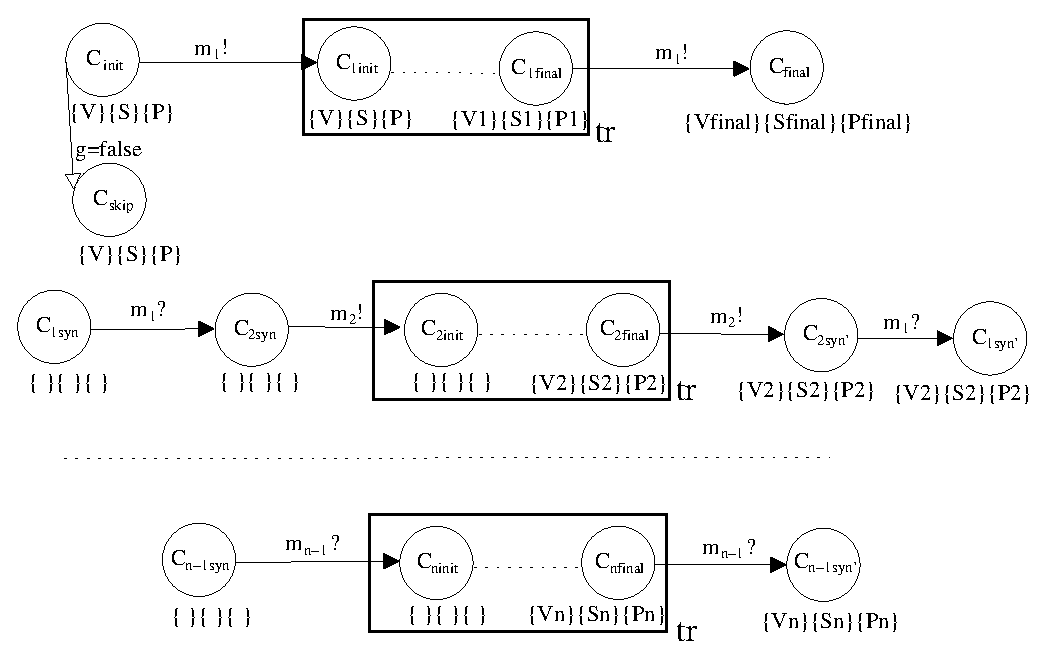
\includegraphics[width=10cm]{Figures/automaton_a8.eps}
%%\end{center}
%%  \caption{NTA corresponding to a \textbf{composition of norms} (AND-refinement)}
%%  \label{automaton_A8}
%%\end{figure}
%%
%%%14
%%\item If several norms are composed by an \textbf{OR-refinement}, that is, we have the diagram $(\epsilon,name,g,tr,C_1 \, Or \, C_2 \, Or \ldots Or \, C_n,\epsilon)$, their composition corresponds to an automaton in which the automata corresponding to each one of the norms is considered as an alternative. Let us consider $\mathcal{C}_1, \mathcal{C}_2, \ldots, \mathcal{C}_n$ the automata corresponding to the norms we are composing. The resulting automaton $\mathcal{OR*}$ preserves the structure of the automata we are composing, adding two nodes called $C_{init}$ and $C_{final}$. We define an urgent edge performing no action for each one of the norms we are composing connecting $C_{init}$ with the initial node of the automaton corresponding to the norm and we also define an urgent edge performing no action for each one of the norm we are composing connecting the final node of its automaton with $C_{final}$. We add another node $C_{skip}$ if guard condition of the parent clause $g \neq \epsilon$ and an urgent edge from $C_{init}$ to this new node guarded with the guard condition negated ($\neg g$). In the final node of this new structure we keep the violation, satisfaction and permission sets of the previous final node, so we have that Vfinal = ${V1 | V2 | \ldots | Vn}$, Sfinal = ${S1 | S2 | \ldots | Sn}$ and Pfinal = ${P1 | P2 | \ldots | Pn}$. If time restriction of the parent clause $tr \neq \epsilon$, we consider this additional time restriction in all the composed automata together with their own time restrictions. Let $\mathcal{C}_1=(N_{\mathcal{C}_1}, n_{0_{\mathcal{C}_1}}, E_{\mathcal{C}_1}, I_{\mathcal{C}_1}), \mathcal{C}_2=(N_{\mathcal{C}_2}, n_{0_{\mathcal{C}_2}}, E_{\mathcal{C}_2}, I_{\mathcal{C}_2}), \ldots,
%%\mathcal{C}_n=(N_{\mathcal{C}_n}, n_{0_{\mathcal{C}_n}}, E_{\mathcal{C}_n}, I_{\mathcal{C}_n})$. Considering the case where $g \neq \epsilon$ and $tr \neq \epsilon$, and having that $E_{\mathcal{C}_1}*, E_{\mathcal{C}_2}*, \ldots ,E_{\mathcal{C}_n}*$ are the sets of edges considering time restriction $tr$ together with their own time restriction, the resulting automaton is therefore $\mathcal{OR*}=(N_{\mathcal{OR*}}, n_{0_{\mathcal{OR*}}}, E_{\mathcal{OR*}}, I_{\mathcal{OR*}})$, where:
%%
%%\begin{itemize}
%%
%%\item $N_{\mathcal{OR*}}=N_{\mathcal{C}_1} \cup N_{\mathcal{C}_2} \cup \ldots \cup N_{\mathcal{C}_n} \cup \{C_{init},C_{final},C_{skip}\}$.
%%
%%\item $n_{0_{\mathcal{OR*}}}=C_{1init}$.
%%
%%\item $E_{\mathcal{OR*}}=E_{\mathcal{C}_1}* \cup E_{\mathcal{C}_2}* \cup \ldots \cup E_{\mathcal{C}_n}* \cup \{C_{init} \flechalu{}{} C_{1init}, C_{init} \flechalu{}{} C_{2init}, \ldots ,$\\
%%$C_{init} \flechalu{}{} C_{ninit}\} \cup \{C_{1final} \flechalu{}{} C_{final}, C_{2final} \flechalu{}{} C_{final}, \ldots ,$\\ $C_{nfinal} \flechalu{}{} C_{final}\} \cup \{C_{init} \flechalu{\neg g}{} C_{skip}\}$.
%%
%%\item $I_{\mathcal{OR*}}=I_{\mathcal{C}_1} \cup \{I(n) \equiv x \leq t2 + 1 \, | \, n \in N_{\mathcal{C}_1}-\{C_{1final}\}\} \cup I_{\mathcal{C}_2} \cup \{I(n) \equiv x \leq t2 + 1 \, | \, n \in N_{\mathcal{C}_2}-\{C_{2final}\}\} \cup \ldots \cup I_{\mathcal{C}_n} \cup \{I(n) \equiv x \leq t2 + 1 \, | \, n \in N_{\mathcal{C}_n}-\{C_{nfinal}\}\}$.
%%
%%\end{itemize}
%%
%%This composition of timed automata is shown graphically in Figure \ref{automaton_A9}.
%%
%%\begin{figure}
%%\begin{center}
%%  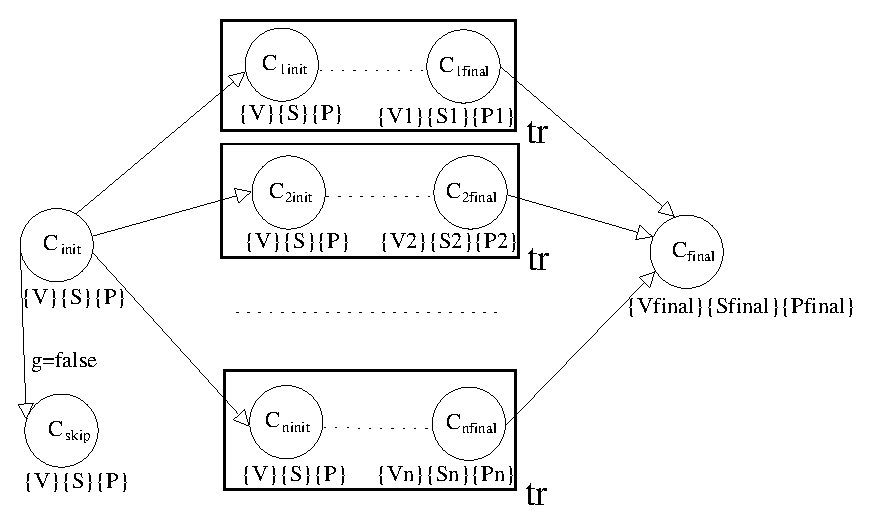
\includegraphics[width=10cm]{Figures/automaton_a9.eps}
%%\end{center}
%%  \caption{Automaton corresponding to a \textbf{composition of norms} (OR-refinement)}
%%  \label{automaton_A9}
%%\end{figure}
%%
%%%15
%%\item If several norms are composed by a \textbf{SEQ-refinement}, that is, we have the diagram $(\epsilon,name,g,tr,C_1 \, Seq \, C_2 \, Seq \ldots Seq \, C_n,\epsilon)$, their composition corresponds to an automaton in which the automata corresponding to
%%each one of the norms are connected in sequence. Let us consider $\mathcal{C}_1, \mathcal{C}_2, \ldots, \mathcal{C}_n$ the automata corresponding to the norms we are composing. The resulting automaton $\mathcal{SEQ*}$ preserves the structure of the automata we are composing, adding just one extra node $C_{skip}$ if guard condition of the parent clause $g \neq \epsilon$ and an urgent edge from $C_{1init}$ to this new node guarded with the guard condition negated ($\neg g$). We connect with an urgent edge performing no action the ending node of each automaton in the sequence ($C_{1final}, C_{2final}, \ldots, C_{n-1final}$) with the initial node of the next automaton ($C_{2init}, C_{3init} \ldots, C_{ninit}$). This rule is not applied in the cases of $C_{1init}$ (as there is not previous ending node to connect) and $C_{nfinal}$ (as there is not following initial node to connect). In the initial node of each one of the composed automata we preserve the violation, satisfaction and permission sets of the previous final node. If time restriction of the parent clause $tr \neq \epsilon$, we consider this additional time restriction in all the composed automata together with their own time restrictions. Let $\mathcal{C}_1=(N_{\mathcal{C}_1}, n_{0_{\mathcal{C}_1}}, E_{\mathcal{C}_1}, I_{\mathcal{C}_1}), \mathcal{C}_2=(N_{\mathcal{C}_2}, n_{0_{\mathcal{C}_2}}, E_{\mathcal{C}_2}, I_{\mathcal{C}_2}), \ldots,
%%\mathcal{C}_n=(N_{\mathcal{C}_n}, n_{0_{\mathcal{C}_n}}, E_{\mathcal{C}_n}, I_{\mathcal{C}_n})$. Considering the case where $g \neq \epsilon$ and $tr \neq \epsilon$, and having that $E_{\mathcal{C}_1}*, E_{\mathcal{C}_2}*, \ldots ,E_{\mathcal{C}_n}*$ are the sets of edges considering time restriction $tr$ together with their own time restriction, the resulting automaton is therefore $\mathcal{SEQ*}=(N_{\mathcal{SEQ*}}, n_{0_{\mathcal{SEQ*}}}, E_{\mathcal{SEQ*}}, I_{\mathcal{SEQ*}})$, where:
%%
%%\begin{itemize}
%%
%%\item $N_{\mathcal{SEQ*}}=N_{\mathcal{C}_1} \cup N_{\mathcal{C}_2} \cup \ldots \cup N_{\mathcal{C}_n} \cup \{C_{skip}\}$.
%%
%%\item $n_{0_{\mathcal{SEQ*}}}=C_{1init}$.
%%
%%\item $E_{\mathcal{SEQ*}}=E_{\mathcal{C}_1}* \cup E_{\mathcal{C}_2}* \cup \ldots \cup E_{\mathcal{C}_n}* \cup \{C_{1init} \flechalu{\neg g}{} C_{skip},C_{1final} \flechalu{}{} C_{2init},$\\
%%$ C_{2final} \flechalu{}{} C_{3init}, \ldots, C_{n-1final} \flechalu{}{} C_{ninit}\}$.
%%
%%\item $I_{\mathcal{SEQ*}}=I_{\mathcal{C}_1} \cup \{I(n) \equiv x \leq t2 + 1 \, | \, n \in N_{\mathcal{C}_1}-\{C_{1final}\}\} \cup I_{\mathcal{C}_2} \cup \{I(n) \equiv x \leq t2 + 1 \, | \, n \in N_{\mathcal{C}_2}-\{C_{2final}\}\} \cup \ldots \cup I_{\mathcal{C}_n} \cup \{I(n) \equiv x \leq t2 + 1 \, | \, n \in N_{\mathcal{C}_n}-\{C_{nfinal}\}\}$.
%%
%%\end{itemize}
%%
%%This composition of timed automata is shown graphically in Figure \ref{automaton_A10}.
%%
%%\begin{figure}
%%\begin{center}
%%  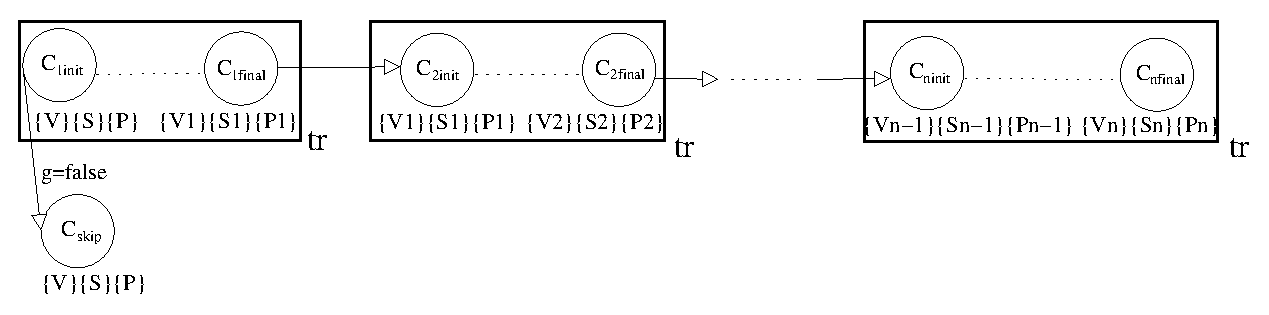
\includegraphics[width=12cm]{Figures/automaton_a10.eps}
%%\end{center}
%%  \caption{Automaton corresponding to a \textbf{composition of norms} (SEQ-refinement)}
%%  \label{automaton_A10}
%%\end{figure}
%%
%%\end{enumerate}
%%
%%}
%%
%%\edfnt
%%
%%\vspace{-2ex}
%%{\flushright $\Box$\\
%%\mbox{}\vspace{-2ex}}
%%
%%\subsection{Implementation in UPPAAL}
%%
%%Once we have defined the semantics of \codiag\ as a translation into an NTA, we would like to be able to check the model we have obtained. We intent to implement the NTAs that we have obtained corresponding to \codiag\ in the UPPAAL tool. In this way, we can take advantage of all the mechanisms for simulation and formal verification provided by the tool.
%%
%%The implementation of the NTAs we have obtained in UPPAAL is quite straightforward as both, the NTA formalism considered by the tool and the NTA formalism that we have considered in the \codiag\ semantics, are very similar. There are only a few implementation points that need a more detail explanation:
%%
%%\begin{itemize}
%%
%%\item First, as there is no way in UPPAAL of directly expressing that an edge without synchronisation should be taken without delay, that is, there are no urgent edges, we have to find an alternative way of encoding this behaviour. For this purpose we consider the modelling pattern proposed in \cite{Behrmann2004}. The encoding of urgent edges introduces an extra automaton, that we call $Urgent$, with a single location and a self loop. The self loop synchronises on an urgent channel that we call $urg\_edge$ (left-hand side of Figure \ref{Automata_Urgent}). An edge can now be made urgent by performing the complimentary action (right-hand side of Figure \ref{Automata_Urgent}).
%%
%%\begin{figure}
%%\begin{center}
%%  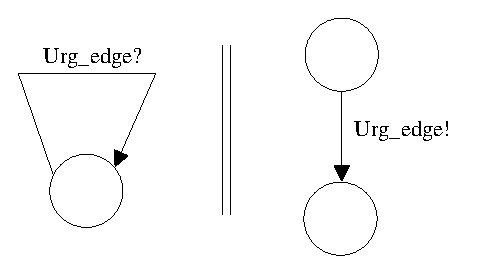
\includegraphics[width=4cm]{Figures/automatonurgent.eps}
%%\end{center}
%%  \caption{Encoding of urgent edges. The $urg\_edge$ channel is declared urgent}
%%  \label{Automata_Urgent}
%%\end{figure}
%%
%%\item The performance of actions by agents is implemented by means of boolean variables in UPPAAL. We define a boolean variable called $agent\_action$ for each one of the actions considered in the contract. These variables are initialized to \textbf{false} and, when one of the actions is performed by an agent in one of the edges, we update the value of the corresponding variable to \textbf{true}.
%%
%%For example, considering an action $a1$ performed by an agent $Seller$, we define the boolean variable $Seller\_a1$ and in the edges of the automata performing this action we update the value of the variable to true ($Seller\_a1=true$).
%%
%%\item Finally, the violation, satisfaction and permission sets are implemented in UPPAAL by means of boolean arrays and constant integers with the names of the clauses of the contract containing obligations, prohibitions or permissions. We define an array $V$ for violation, an array $S$ for satisfaction, and an array $P$ for permission, all of them initialized to \textbf{false}. The size of the arrays $V$ and $S$ is equal to the number of obligations and prohibitions in the contract, whereas the size of the array $P$ is equal to the number of permissions. We also define constant integers with the name of the clauses containing obligations and prohibitions, initializing each one of them to a different value (from 0 to the size of the arrays $V$ and $S$ minus 1), and constant integers with the name of the clauses containing permissions, initializing each one of them to a different value (from 0 to the size of the array $P$ minus 1). These constants are used as indexes in the arrays.
%%When we move in the automata to a node where one of the sets is modified (an obligation/prohibition is violated, an obligation/prohibition is satisfied or a permission is made effective), in the edge reaching this node we update to \textbf{true} in the proper array the value of the index corresponding to the clause. In the case of repairing an obligation/prohibition violation, the index corresponding to the proper clause in $V$ is set to \textbf{false}.
%%
%%For example, if we consider a clause $Send\_Item$ specifying the obligation of sending an item within a concrete time frame, when the time expires and we move in the NTA to a node where this clause is add to the violation set, in the edge reaching this node we include the update $V[Send\_Item]=true$.
%%
%%\end{itemize}
%%
%%%%%OAP case study%%%
%%\section{Case Study: Online Auctioning Process}\label{OAP}
%%\markright{~\ref{OAP} Case Study: Online Auctioning Process}
%%
%%%%OAP description%%
%%The case study presented in this section is inspired by the motivating example described in \cite{Decker2009}. It consists of an \textit{Online Auctioning Process} involving the interaction between three different agents: the \textit{buyer}, the \textit{seller}, and the \textit{auction service}.
%%
%%The description of the process we are considering here is the following: the online auctioning starts when a \textit{seller} wants to auction an item. Therefore, the \textit{seller} has \textbf{one day} to upload valid information about the item he wants to sell, being forbidden the sale of inadequate items such as replicas of designers items or wild animals. Once it has been checked that the item can be auctioned, the \textit{auction service} also has \textbf{one day} to publish the auction of the item. After that, the \textit{buyer} can place bids during \textbf{seven days}. When this period of time is over, if the bid placed by the \textit{buyer} is the highest one, the activities concerning the payment and the shipment of the item start.
%%
%%First, the \textit{buyer} has \textbf{three days} to perform the payment, which can be done by means of credit card or PayPal. After the payment has been performed, the \textit{seller} has \textbf{fourteen days} to send the item to the \textit{buyer}. If the item is not received within this period of time, the \textit{auction service} has \textbf{seven days} to refund the payment to the \textit{buyer} and can penalize the \textit{seller} in some way (for example not allowing the \textit{seller} to auction new items for a period of time). However, if the reception of the item by the \textit{buyer} is acknowledge on time, the auction process is considered finished successfully.
%%
%%%%OAP list of clauses%%
%%In Table \ref{Norms2} we show a list of the obligations, permissions and prohibitions that can be inferred from the description of the process. In this table we can see that there are nine clauses specifying real-time constraints. In \textbf{Clause 2} and \textbf{Clause 3} it is specified that after selecting an item to auction (\textbf{Clause 1}), the \textit{buyer} has one day to upload valid information about the item, being forbidden to auction an inadequate item. In \textbf{Clause 4} we have that the \textit{auction service} has one day to publish the auction of the item after it has been checked (\textbf{Clause 2} and \textbf{Clause 3}). In \textbf{Clause 5} we have that the \textit{buyer} is allowed to place bids for the item during seven days after publication (\textbf{Clause 4}). In \textbf{Clause 6} and \textbf{Clause 7} it is specified that the \textit{buyer} has three days to pay the item (respectively by credit card or PayPal) after winning the auction. \textbf{Clause 8} specifies that the \textit{seller} has fourteen days to send the item to the \textit{buyer} after payment (\textbf{Clause 6} or \textbf{Clause 7}). Finally, \textbf{Clause 9} and \textbf{Clause 10} specify that the \textit{auction service} has seven days to refund the payment to the \textit{buyer} if the item is not received on time and can penalize the \textit{seller} in this period of time. We can also see in Table \ref{Norms2} that \textbf{Clause 6}, \textbf{Clause 7} and \textbf{Clause 8} are conditioned to the result of the auction, that is, they are only applied if the \textit{buyer} has won the auction. In the case of the obligation specified by \textbf{Clause 8} we can see that there is a possible reparation for the violation of this clause consisting of the obligation specified by \textbf{Clause 9} and the permission specified by \textbf{Clause 10}.
%%
%%\begin{table}
%%\small
%%\begin{center}
%%
%%\begin{tabular}{|p{1.1cm}|p{1.4cm}|p{1.8cm}|p{1.6cm}|p{1.7cm}|p{1.6cm}|p{2.8cm}|}
%%
%%\hline
%%
%%\begin{center}\textbf{Clause}\end{center} & \begin{center}\textbf{Agent}\end{center} & \begin{center}\textbf{Modality}\end{center} & \begin{center}\textbf{Action}\end{center} & 
%%\begin{center}\textbf{Condition}\end{center} & \begin{center}\textbf{Time}\end{center} & \begin{center}\textbf{Reparation}\end{center}\\
%%
%%\hline
%%
%%\begin{center}\textbf{1}\end{center} & \begin{center}\textit{Seller}\end{center} & \begin{center}\textit{Permission}\end{center} & Can select an item to auction & 
%%\begin{center}$\emptyset$\end{center} & \begin{center}$\emptyset$\end{center} &
%%\begin{center}$\emptyset$\end{center}\\
%%
%%\hline
%%
%%\begin{center}\textbf{2}\end{center} & \begin{center}\textit{Seller}\end{center} & \begin{center}\textit{Prohibition}\end{center} & Auctions a fraudulent item &
%%\begin{center}$\emptyset$\end{center} & One day after selection ($t_1$) &
%%\begin{center}$\emptyset$\end{center}\\
%%
%%\hline
%%
%%\begin{center}\textbf{3}\end{center} & \begin{center}\textit{Seller}\end{center} & \begin{center}\textit{Obligation}\end{center} & Uploads valid information about item & 
%%\begin{center}$\emptyset$\end{center} & One day after selection ($t_1$) &
%%\begin{center}$\emptyset$\end{center}\\
%%
%%\hline
%%
%%\begin{center}\textbf{4}\end{center} & \begin{center}\textit{Auction Service}\end{center} & \begin{center}\textit{Obligation}\end{center} & Publishes the auction of the item & 
%%\begin{center}$\emptyset$\end{center} & One day after checked ($t_2$) &
%%\begin{center}$\emptyset$\end{center}\\
%%
%%\hline
%%
%%\begin{center}\textbf{5}\end{center} & \begin{center}\textit{Buyer}\end{center} & 
%%\begin{center}\textit{Permission}\end{center} & Can place bids for the item &
%%\begin{center}$\emptyset$\end{center} & Seven days after publication ($t_3$) &
%%\begin{center}$\emptyset$\end{center}\\
%%
%%\hline
%%
%%\begin{center}\textbf{6}\end{center} & \begin{center}\textit{Buyer}\end{center} & 
%%\begin{center}\textit{Obligation}\end{center} & Pays the item by credit card & 
%%The bid placed is the highest ($g_1$) & Three days after auction ($t_4$) &
%%\begin{center}$\emptyset$\end{center}\\
%%
%%\hline
%%
%%\begin{center}\textbf{7}\end{center} & \begin{center}\textit{Buyer}\end{center} &
%%\begin{center}\textit{Obligation}\end{center} & Pays the item by PayPal & 
%%The bid placed is the highest ($g_1$) & Three days after auction ($t_4$) &
%%\begin{center}$\emptyset$\end{center}\\
%%
%%\hline
%%
%%\begin{center}\textbf{8}\end{center} & \begin{center}\textit{Seller}\end{center} & \begin{center}\textit{Obligation}\end{center} & Sends the item to the \textit{buyer}& 
%%The bid placed is the highest ($g_1$) & Fourteen days after auction ($t_5$) &
%%\begin{center}\emph{CLAUSE 9} and \emph{CLAUSE 10} ($R_1$)\end{center}\\
%%
%%\hline
%%
%%\begin{center}\textbf{9}\end{center} & \begin{center}\textit{Auction service}\end{center} & \begin{center}\textit{Obligation}\end{center} & Refunds the payment to the \textit{buyer} &
%%\begin{center}$\emptyset$\end{center} & Seven days after violation of \emph{CLAUSE 8} ($t_6$) &
%%\begin{center}$\emptyset$\end{center}\\
%%
%%\hline
%%
%%\begin{center}\textbf{10}\end{center} & \begin{center}\textit{Auction service}\end{center} & \begin{center}\textit{Permission}\end{center} & Can penalize the \textit{seller} of the item & 
%%\begin{center}$\emptyset$\end{center} & Seven days after violation of \emph{CLAUSE 8} ($t_6$) &
%%\begin{center}$\emptyset$\end{center}\\
%%
%%\hline
%%
%%\end{tabular}
%%
%%\caption{Norms of the \textit{Online Auctioning Process} contract}
%%\label{Norms2}
%%
%%\end{center}
%%
%%\end{table}
%%
%%%%OAP diagrams%%
%%What follows we model this contract with \codiag\ taking into account the information provided in Table \ref{Norms2}. In these diagrams we use $a_n$ to denote the action corresponding to clause number $n$ and the reparation for \textbf{Clause 8} is called $R_1$. We also use $t_1$ to denote the real-time constraint of \textbf{Clause 2} and \textbf{Clause 3}, $t_2$ to denote the real-time constraint of \textbf{Clause 4}, $t_3$ to denote the real-time constraint of \textbf{Clause 5}, $t_4$ to denote the real-time constraint of \textbf{Clause 6} and \textbf{Clause 7}, $t_5$ to denote the real-time constraint of \textbf{Clause 8}, and $t_6$ to denote the real-time constraint of \textbf{Clause 9}. The condition of placing the highest bid is denoted as $g_1$.
%%
%%In Figure \ref{OAP1} we show the top-level of the \textit{C-O Diagram} we specify for the process, called \textit{Online\_Auctioning}, starting the sequence from the permission specified in \textbf{Clause 1}, that has been called \textit{Auction\_Item}. We have grouped the rest of the clauses in Table \ref{Norms2} (except the ones corresponding to the reparation) into three more general clauses with a sequence relationship between them: \textit{Check\_Item} (\textbf{Clause 2} and \textbf{Clause 3}), \textit{Auction\_Process} (\textbf{Clause 4} and \textbf{Clause 5}), and \textit{Payment\_Shipment} (\textbf{Clause 6}, \textbf{Clause 7} and \textbf{Clause 8}). These general clauses cover the different phases that we have identified in the \textit{Online Auctioning Process}.
%%
%%\begin{figure}
%%\begin{center}
%%  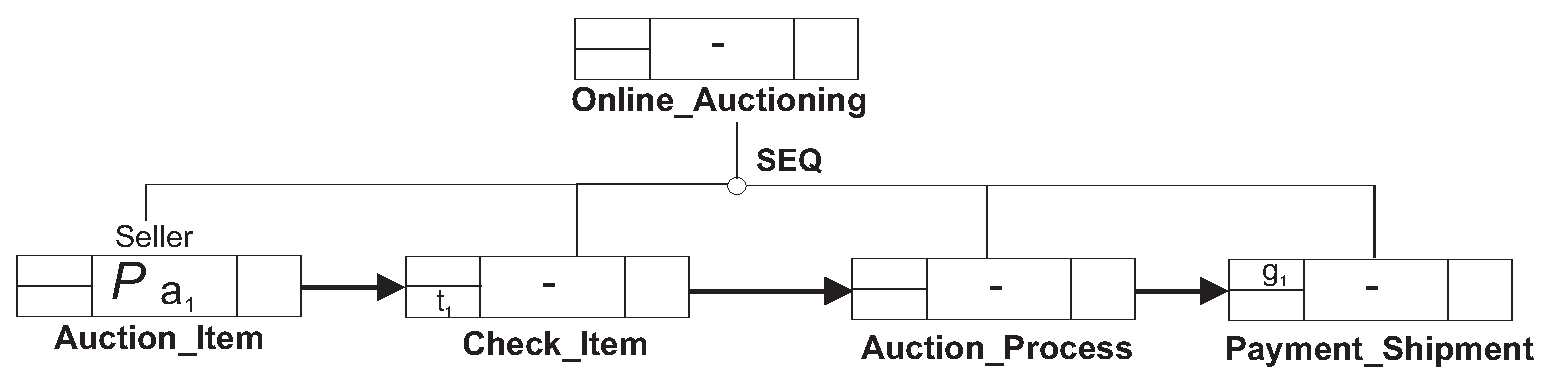
\includegraphics[width=12cm]{Figures/OnlineAuctioning1.eps}
%%\end{center}
%%  \caption{Top-level of the \textit{C-O Diagram} for the \textit{Online Auctioning Process}}
%%  \label{OAP1}
%%\end{figure}
%%
%%The decomposition of clause \textit{Check\_Item} into subclauses can be seen in Figure \ref{OAP2}, where an \textit{AND-refinement} is used in the decomposition and the real-time constraint $t_1$ is affecting the whole composition. We have on the left-hand side the specification of the prohibition specified in \textbf{Clause 2}, that has been called \textit{Inadequate\_Item}, and on the right-hand side the obligation specified in \textbf{Clause 3}, that has been called \textit{Valid\_Information}.
%%
%%\begin{figure}
%%\begin{center}
%%  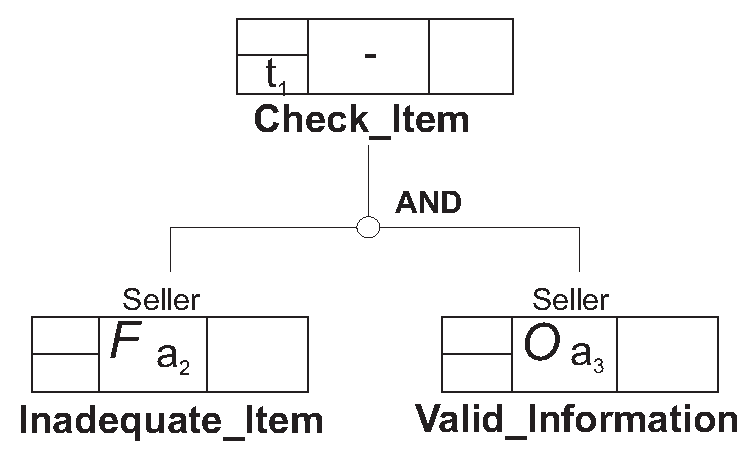
\includegraphics[width=8cm]{Figures/OnlineAuctioning2.eps}
%%\end{center}
%%  \caption{Decomposition of clause \textit{Check\_Item}}
%%  \label{OAP2}
%%\end{figure}
%%
%%The decomposition of clause \textit{Auction\_Process} into subclauses can be seen in Figure \ref{OAP3}, where a \textit{SEQ-refinement} is used in the decomposition. We have on the left-hand side the specification of the obligation specified in \textbf{Clause 4}, that has been called \textit{Publish\_Item}, including the real-time constraint $t_2$, and on the right-hand side the permission specified in \textbf{Clause 5}, that has been called \textit{Place\_Bid}, including the real-time constraint $t_3$. We can see in this clause that the repetition structure of \codiag\ is used to model that the \textit{buyer} is allowed to place multiple bids.
%%
%%\begin{figure}
%%\begin{center}
%%  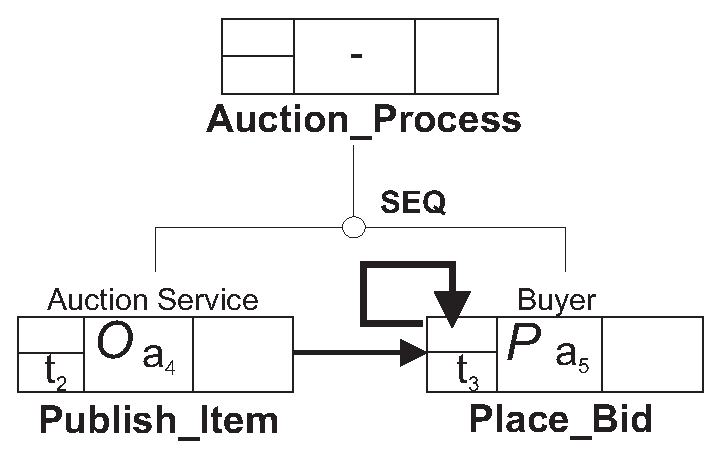
\includegraphics[width=8cm]{Figures/OnlineAuctioning3.eps}
%%\end{center}
%%  \caption{Decomposition of clause \textit{Auction\_Process}}
%%  \label{OAP3}
%%\end{figure}
%%
%%The decomposition of clause \textit{Payment\_Shipment} into subclauses can be seen in Figure \ref{OAP4}, where a \textit{SEQ-refinement} is used again in the decomposition and the evaluation of the condition $g_1$ is taken into account for the application of the clauses. We have on the left-hand side the obligation specified in \textbf{Clause 6} and \textbf{Clause 7} about the payment, that has been called \textit{Payment\_Item}, including the real-time constraint $t_4$ and composing the actions of paying by credit card or PayPal by means of an \textit{OR-refinement}. On the right-hand side we have the obligation specified in \textbf{Clause 8}, that has been called \textit{Send\_Item}, including the real-time constraint $t_5$ and a reference to reparation $R_1$.
%%
%%\begin{figure}
%%\begin{center}
%%  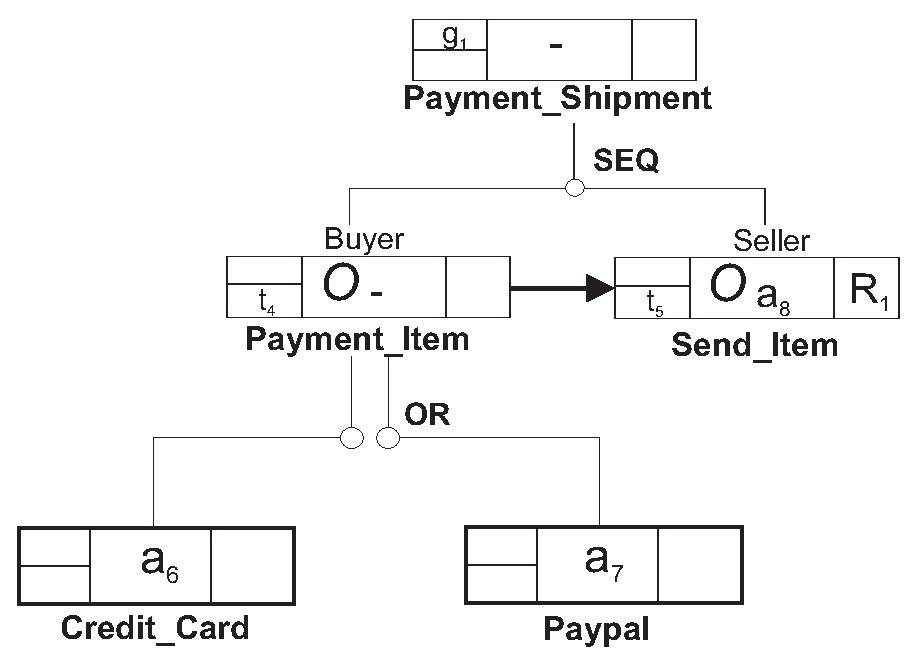
\includegraphics[width=8cm]{Figures/OnlineAuctioning4.eps}
%%\end{center}
%%  \caption{Decomposition of clause \textit{Payment\_Shipment}}
%%  \label{OAP4}
%%\end{figure}
%%
%%Finally, in Figure \ref{OAP5} we can see the diagram corresponding to reparation $R_1$. It has been called \textit{Refund\_Penalty}, including the real-time constraint $t_6$, and it is decomposed into two subclauses by means of an \textit{AND-refinement}. The subclause on the left corresponds to the obligation specified in \textbf{Clause 9}, that has been called \textit{Refund\_Buyer}, and the subclause on the right corresponds to the permission specified in \textbf{Clause 10}, that has been called \textit{Penalty\_Seller}.
%%
%%\begin{figure}
%%\begin{center}
%%  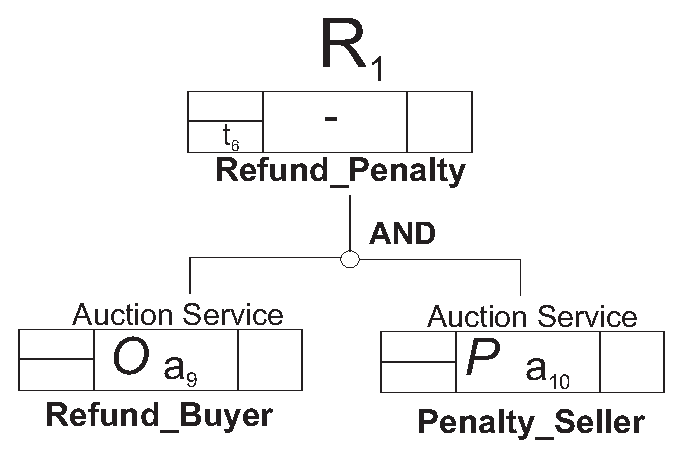
\includegraphics[width=6cm]{Figures/OnlineAuctioning5.eps}
%%\end{center}
%%  \caption{Reparation of clause \textit{Send\_Item} called \textit{Refund\_Penalty}}
%%  \label{OAP5}
%%\end{figure}
%%
%%%%OAP automata construction%%
%%
%%Next, we are going to show how this contract is translated into a network of timed automata according to the \codiag\ semantics, where the basic transformation rule \textbf{(1)} is applied to obtain an edge executing each one of the actions considered in the contract.
%%
%%\begin{figure}
%%\begin{center}
%%  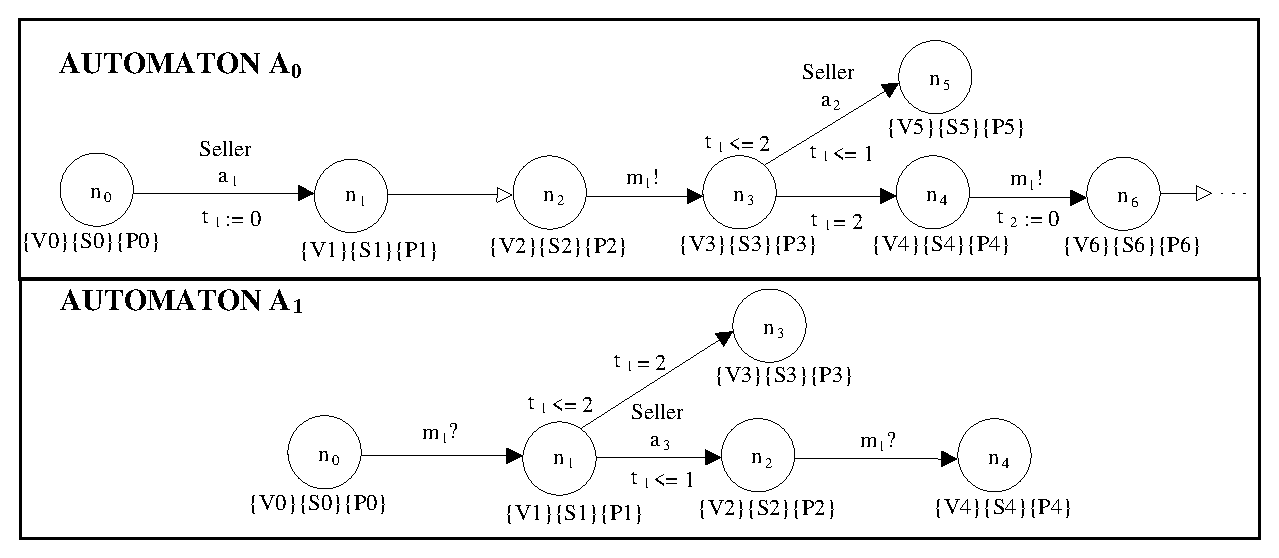
\includegraphics[width=12cm]{Figures/AutomatonOAP1.eps}
%%\end{center}
%%  \caption{First part of automaton $A_0$ and automaton $A_1$}
%%  \label{AutomatonOAP1}
%%\end{figure}
%%
%%In Figure \ref{AutomatonOAP1} we can see the translation into automata corresponding to the first part of the contract. In the initial state $n_0$ of main automaton $A_0$ we have that the violation, satisfaction and permission sets are empty ($V0=\{\}$, $S0=\{\}$ and $P0=\{\}$).
%%
%%As the first norm of the contract is a permission over an action without time restriction nor guard, by applying the transformation rule \textbf{(6)} we obtain the state $n_1$ of $A_0$, adding the clause \textit{Auction\_Item} to its permission set ($V1=\{\}$, $S1=\{\}$ and $P1=\{Auction\_Item\}$), and the edge from $n_0$ to $n_1$ performing agent \textbf{seller} action $a_1$. In this edge the clock $t_1$, used to model the time restriction with the same name, is reset.
%%
%%Considering that there is a \textbf{SEQ-refinement} connecting this first norm with the rest of the contract, by applying rule \textbf{(15)} we connect state $n_1$ of $A_0$ with state $n_2$ of $A_0$ by means of an urgent edge, keeping in $n_2$ the same sets that in $n_1$.
%%
%%As the next part of the contract consists of an \textbf{AND-refinement} composing two different norms, the transformation rule \textbf{(13)} is applied, defining a new automaton $A_1$ to execute in parallel with the main automaton $A_0$. The edge from $n_2$ to $n_3$ in $A_0$ and the edge from $n_0$ to $n_1$ in $A_1$ are used to synchronize by means of the channel $m_1$. Now we have on the one hand the prohibition over an action considered in automaton $A_0$ by applying rule \textbf{(7)}, and on the other hand the obligation over an action considered in automaton $A_1$ by applying rule \textbf{(5)}. 
%%
%%Concerning the prohibition in $A_0$, in the node $n_3$ we keep the same sets that in $n_2$ and, as time restriction $t_1$ is specified for the norm, the invariant $t_1 \leq 2$ is defined in the node. Next, we have an edge from $n_3$ to $n_5$ considering the performance by agent \textbf{seller} of the forbidden action $a_2$ with the guard $t_1 \leq 1$, so in $n_5$ the clause \textit{Inadequate\_Item} is added to the violation set ($V5=\{Inadequate\_Item\}$, $S5=\{\}$ and $P5=\{Auction\_Item\}$), having that $n_5$ is a final node of the whole automaton as no reparation is defined for the prohibition and the contract is breached. However, we also have an edge from $n_3$ to $n_4$ considering that the forbidden action is not executed with the guard $t_1 = 2$, so in $n_4$ the clause \textit{Inadequate\_Item} is added to the satisfaction set ($V4=\{\}$, $S4=\{Inadequate\_Item\}$ and $P4=\{Auction\_Item\}$).
%%
%%In the automaton $A_1$, where we consider the obligation, we have that nodes $n_0$ and $n_1$ have empty violation, satisfaction and permission sets and, as time restriction $t_1$ is specified for the norm, the invariant $t_1 \leq 2$ is included in $n_1$. Next, we have an edge from $n_1$ to $n_2$ considering the performance by agent \textbf{seller} of the obliged action $a_3$ with the guard $t_1 \leq 1$, so in $n_2$ the clause \textit{Valid\_Information} is added to the satisfaction set ($V2=\{\}$, $S2=\{Valid\_Information\}$ and $P2=\{\}$). We also have an edge from $n_1$ to $n_3$ considering that the obliged action is not executed with the guard $t_1 = 2$, so in $n_3$ the clause \textit{Valid\_Information} is added to the violation set ($V3=\{Valid\_Information\}$, $S3=\{\}$ and $P3=\{\}$), having that $n_3$ is also a final node where the contract is breached.
%%
%%Finally, to synchronize both automata again by means of channel $m_1$, we have the edge from $n_4$ to $n_6$ in $A_0$ (resetting the clock $t_2$ used to model the time restriction with the same name) and the edge from $n_2$ to $n_4$ in $A_1$. In node $n_4$ in $A_1$ we keep the sets of $n_2$, but in node $n_6$ in $A_0$ we add \textit{Valid\_Information} to its satisfaction set ($V6=\{\}$, $S6=\{Inadequate\_Item,Valid\_Information\}$ and $P6=\{Auction\_Item\}$).
%%
%%\begin{figure}
%%\begin{center}
%%  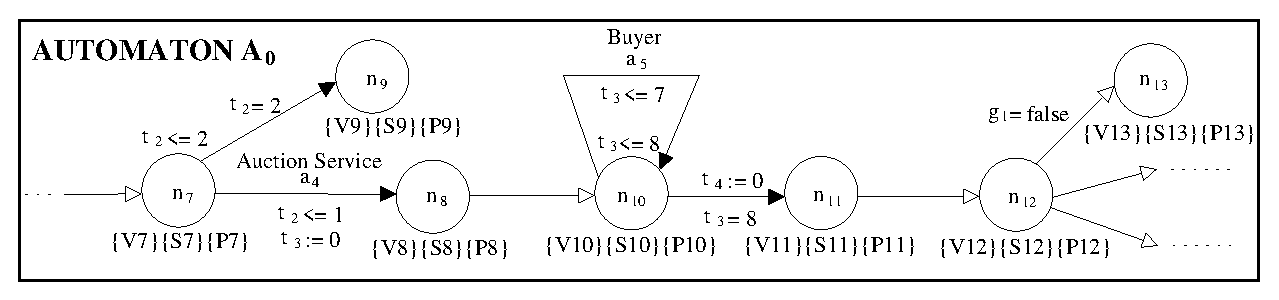
\includegraphics[width=12cm]{Figures/AutomatonOAP2.eps}
%%\end{center}
%%  \caption{Second part of automaton $A_0$}
%%  \label{AutomatonOAP2}
%%\end{figure}
%%
%%In Figure \ref{AutomatonOAP2} we can see the automaton corresponding to the second part of the contract, that is, starting from clause \textit{Auction\_Process}. We first have that the node $n_7$ is connected to node $n_6$ by means of an urgent edge as there is a \textbf{SEQ-refinement} connecting this part of the contract with the previous norms, preserving in node $n_7$ the same sets that in $n_6$. Considering that the next norm in the contract is an obligation over an action with time restriction $t_2$, we apply rule \textbf{(5)}, adding to node $n_7$ the invariant $t_2 \leq 2$. Next, we have an edge from $n_7$ to $n_8$ considering the performance by agent \textbf{auction service} of the obliged action $a_4$ with the guard $t_2 \leq 1$ (and resetting the clock $t_3$ used to model the time restriction with the same name), so in $n_8$ the clause \textit{Publish\_Item} is added to the satisfaction set ($V8=\{\}$, $S8=\{Inadequate\_Item,Valid\_Information,Publish\_Item\}$ and $P8=\{Auction\_Item\}$). We also have an edge from $n_7$ to $n_9$ considering that the obliged action is not executed with the guard $t_2 = 2$, so in $n_9$ the clause \textit{Publish\_Item} is added to the violation set and the contract is breached again ($V9=\{Publish\_Item\}$,$S9=\{Inadequate\_Item, Valid\_Information\}$ and $P9=\{Auction\_Item\}$).
%%
%%After that, the node $n_8$ is connected to node $n_{10}$ by means of an urgent edge as there is a \textbf{SEQ-refinement} connecting the norms of the clause \textit{Auction\_Process}, preserving in node $n_{10}$ the same sets that in $n_8$. As the next norm in the contract is a permission over an action, we apply rule \textbf{(6)}, but taking into account that this time the permission includes a time restriction $t_3$ and it is applied repetitively. Therefore, we first add the invariant $t_3 \leq 8$ to node $n_{10}$. An edge from $n_{10}$ to itself is added performing agent \textbf{buyer} the action $a_5$ with the guard $t_3 \leq 7$, so after performing this action for the first time we have that clause \textit{Place\_Bid} is added to the permission set of the node $n_{10}$ ($V10=\{\}$, $S10=\{Inadequate\_Item,Valid\_Information,Publish\_Item\}$ and $P10=\{Auction\_Item,Place\_Bid\}$). Another edge from $n_{10}$ to $n_{11}$ is added with the guard $t_3 = 8$ (and resetting the clock $t_4$ used to model the time restriction with the same name), keeping in $n_{11}$ the same sets that in $n_{10}$.
%%
%%Finally, the node $n_{11}$ is connected to node $n_{12}$ by means of an urgent edge as there is a \textbf{SEQ-refinement} connecting the clause \textit{Auction\_Process} with the next part of the contract, preserving in node $n_{12}$ the same sets that in $n_{11}$. At this point we have in the contract an obligation over a compound action in clause \textit{Payment\_Item} with time restriction $t_4$, where the actions are composed by means of an \textbf{OR-refinement}, so we now apply the translation rules \textbf{(3)} and \textbf{(5)}. First, as the guard condition $g_1$ is considered for the rest of the contract, an urgent edge from $n_{12}$ to $n_{13}$ is added with the guard $g_1=false$. In $n_{13}$ we keep the violation, satisfaction and permission sets that we have in $n_{12}$ and the automaton ends (but in this case the contract is not breached). The other two urgent edges going out of $n_{12}$ correspond to the choice of performing one of the obliged actions or the other when the guard $g_1=true$ is satisfied.
%%
%%\begin{figure}
%%\begin{center}
%%  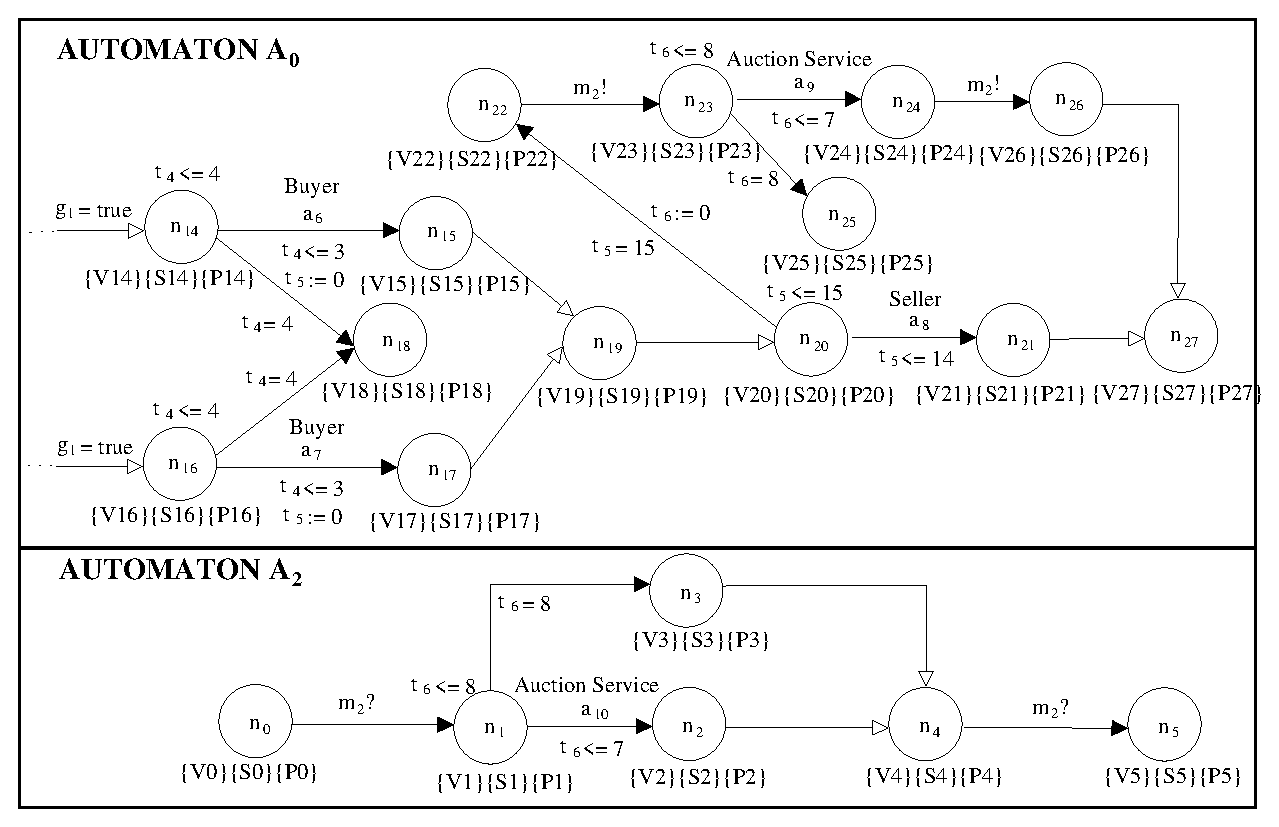
\includegraphics[width=12cm]{Figures/AutomatonOAP3.eps}
%%\end{center}
%%  \caption{Third part of automaton $A_0$ and automaton $A_2$}
%%  \label{AutomatonOAP3}
%%\end{figure}
%%
%%In Figure \ref{AutomatonOAP3} we can see that when it is chosen the performance of the obliged action $a_6$, the automaton moves to state $n_{14}$ where we keep the same sets that in $n_{12}$ and the invariant $t_4 \leq 4$ is included. Next, we have an edge from $n_{14}$ to $n_{15}$ considering the performance of $a_6$ by agent \textbf{buyer} with the guard $t_4 \leq 3$ (and resetting the clock $t_5$ used to model the time restriction with the same name), so in $n_{15}$ the clause \textit{Payment\_Item} is added to the satisfaction set ($V15=\{\}$, $S15=\{Inadequate\_Item, Valid\_Information,Publish\_Item,Payment\_Item\}$ and $P15=\{Auction\_Item,Place\_Bid\}$). We also have an edge from $n_{14}$ to $n_{18}$ where the action $a_6$ is not executed with the guard $t_4 = 4$, so in $n_{18}$ the clause \textit{Payment\_Item} is added to the violation set and the contract is breached:
%%
%%\begin{itemize} 
%%
%%\item $V18=\{Payment\_Item\}$
%%
%%\item $S18=\{Inadequate\_Item, Valid\_Information,Publish\_Item\}$
%%
%%\item $P18=\{Auction\_Item,Place\_Bid\}$
%%
%%\end{itemize}
%%
%%If it is chosen the performance of the obliged action $a_7$ instead of $a_6$, the automaton goes to state $n_{16}$ where we keep the same sets that in $n_{12}$ and the invariant $t_4 \leq 4$ is included. Next, we have an edge from $n_{16}$ to $n_{17}$ considering the performance of $a_7$ by agent \textbf{buyer} with the guard $t_4 \leq 3$ (and resetting the clock $t_5$), so in $n_{17}$ the clause \textit{Payment\_Item} is added to the satisfaction set ($V17=\{\}$, $S17=\{Inadequate\_Item, Valid\_Information,Publish\_Item,Payment\_Item\}$ and $P17=\{Auction\_Item,Place\_Bid\}$). We also have an edge from $n_{16}$ to $n_{18}$ considering that the obliged action is not executed with the guard $t_4 = 4$, having $n_{18}$ the same sets that we have already defined in the other case.
%%
%%After performing action $a_7$ we have an urgent edge from $n_{15}$ to $n_{19}$ and after performing $a_6$ we have another urgent edge from $n_{17}$ to $n_{19}$. In state $n_{19}$ we keep the same sets that we have in $n_{15}$ and $n_{17}$. Next, as there is a \textbf{SEQ-refinement} connecting the clause \textit{Payment\_Item} with the last clause of the contract, $n_{19}$ is connected to $n_{20}$ by means of an urgent edge, preserving in node $n_{20}$ the same sets that in $n_{19}$. At this point we have in the contract an obligation over an action with time restriction $t_5$, so we apply rule \textbf{(5)} again, adding to node $n_{20}$ the invariant $t_5 \leq 15$. Next, we have an edge from $n_{20}$ to $n_{21}$ considering the performance by agent \textbf{seller} of the obliged action $a_8$ with the guard $t_5 \leq 14$, so in $n_{21}$ the clause \textit{Send\_Item} is added to the satisfaction set:
%%
%%\begin{itemize} 
%%
%%\item $V21=\{\}$
%%
%%\item $S21=\{Inadequate\_Item, Valid\_Information,Publish\_Item,\\
%%	Payment\_Item,Send\_Item\}$
%%
%%\item $P21=\{Auction\_Item,Place\_Bid\}$
%%
%%\end{itemize}
%%
%%We also have an edge from $n_{20}$ to $n_{22}$ considering that the obliged action is not executed with the guard $t_5 = 15$ (and resetting the clock $t_6$ used to model the time restriction with the same name), so in $n_{22}$ the clause \textit{Send\_Item} is added to the violation set::
%%
%%\begin{itemize} 
%%
%%\item $V22=\{Send\_Item\}$
%%
%%\item $S22=\{Inadequate\_Item, Valid\_Information,Publish\_Item,\\
%%	Payment\_Item\}$
%%
%%\item $P22=\{Auction\_Item,Place\_Bid\}$
%%
%%\end{itemize}
%%
%%However, in this case $n_{22}$ is not a final node of the automaton as reparation $R_1$ has been defined for the clause \textit{Send\_Item} and we apply rule \textbf{(8)}. Therefore, considering $n_{22}$ the starting node of the reparation contract, as this contract consists of an \textbf{AND-refinement} composing two different norms, the transformation rule \textbf{(13)} is applied, defining a new automaton $A_2$ to execute in parallel with the main automaton $A_0$. The edge from $n_{22}$ to $n_{23}$ in $A_0$ and the edge from $n_0$ to $n_1$ in $A_2$ are used to synchronize by means of channel $m_2$. Now we have on the one hand the obligation over an action considered in automaton $A_0$ by applying rule \textbf{(5)}, and on the other hand the permission over an action considered in automaton $A_2$ by applying rule \textbf{(6)}. In both cases we take into account the time restriction $t_6$.
%%
%%Concerning the obligation in $A_0$, in the node $n_{23}$ we keep the same sets that in $n_{22}$ and we include the invariant $t_6 \leq 8$.  Next, we have an edge from $n_{23}$ to $n_{24}$ considering the performance by agent \textbf{auction service} of the obliged action $a_9$ with the guard $t_6 \leq 7$, so in $n_{24}$ the clause \textit{Refund\_Buyer} is added to the satisfaction set:
%%
%%\begin{itemize} 
%%
%%\item $V24=\{Send\_Item\}$
%%
%%\item $S24=\{Inadequate\_Item, Valid\_Information,Publish\_Item,\\
%%	Payment\_Item,Refund\_Buyer\}$
%%
%%\item $P24=\{Auction\_Item,Place\_Bid\}$
%%
%%\end{itemize}
%%
%%We also have an edge from $n_{23}$ to $n_{25}$ considering that the obliged action is not executed with the guard $t_6 = 8$, so in $n_{25}$ the clause \textit{Refund\_Buyer} is added to the violation set and the contract is breached as no reparation is defined for this new violation of the contract:
%%
%%\begin{itemize} 
%%
%%\item $V25=\{Send\_Item,Refund\_Buyer\}$
%%
%%\item $S25=\{Inadequate\_Item, Valid\_Information,Publish\_Item,\\
%%	Payment\_Item\}$
%%
%%\item $P25=\{Auction\_Item,Place\_Bid\}$
%%
%%\end{itemize}
%%
%%In the automaton $A_2$, where we consider the permission, we have that nodes $n_0$ and $n_1$ have empty violation, satisfaction and permission sets and the invariant $t_6 \leq 8$ is included in $n_1$. Next, we have an edge from $n_1$ to $n_2$ considering the performance by agent \textbf{auction service} of the action $a_{10}$ with the guard $t_6 \leq 7$, so in $n_2$ the clause \textit{Penalty\_Seller} is added to the permission set ($V2=\{\}$, $S2=\{\}$ and $P2=\{Penalty\_Seller\}$). We also have an edge from $n_1$ to $n_3$ considering that the permitted action is not executed with the guard $t_6 = 8$, so in $n_3$ the clause \textit{Penalty\_Seller} is not added and the violation, satisfaction and permission sets remains empty. Next, according to rule \textbf{(11)}, we add an urgent edge from $n_2$ to $n_4$ and another urgent edge from $n_3$ to $n_4$, keeping in the node $n_4$ the sets of the previous node.
%%
%%After that, to synchronize both automata again by means of channel $m_2$, we have the edge from $n_{24}$ to $n_{26}$ in $A_0$ and the edge from $n_4$ to $n_5$ in $A_2$. In node $n_5$ in $A_2$ we keep the sets of $n_4$, but in node $n_{26}$ in $A_0$ we modify the sets of $n_{24}$ by removing clause \textit{Send\_Item} from its violation set and adding to its permission set the clause \textit{Penalty\_Seller} if it has been made effective:
%%
%%\begin{itemize} 
%%
%%\item $V26=\{\}$
%%
%%\item $S26=\{Inadequate\_Item, Valid\_Information,Publish\_Item,\\
%%	Payment\_Item,Refund\_Buyer,Penalty\_Seller\}$
%%
%%\item $P26=\{Auction\_Item,Place\_Bid,Penalty\_Seller?\}$
%%
%%\end{itemize}
%%
%%Finally, according to rule \textbf{(10)}, we add an urgent edge from $n_{21}$ to $n_{27}$ and another urgent edge from $n_{26}$ to $n_{27}$, keeping in the node $n_{27}$ the sets of the previous node, that is, the sets of $n_{21}$ or the sets of $n_{26}$. This is the main final node of the structure we have built, where we have that the contract has been fulfilled and the process ends.
%%
%%%%OAP case study validation and verification%%
%%\subsection{Validation and Verification}
%%
%%The automata we have obtained modelling the contractually correct behaviours of the \textit{Online Auctioning Process} are implemented in the UPPAAL tool as shown in Figure \ref{AutomatonOAP_A0} (Automaton $A_0$), Figure \ref{AutomatonOAP_A1} (Automaton $A_1$) and Figure \ref{AutomatonOAP_A2} (Automaton $A_2$). We omit the automaton $Urgent$ used just for synchronizations with the urgent channel $urg\_edge$.
%%
%%\begin{figure}
%%\begin{center}
%%  \includegraphics[width=12cm]{Figures/AutomatonOAP_A0.eps}
%%\end{center}
%%  \caption{Automaton $A_0$ in UPPAAL}
%%  \label{AutomatonOAP_A0}
%%\end{figure}
%%
%%\begin{figure}
%%\begin{center}
%%  \includegraphics[width=6cm]{Figures/AutomatonOAP_A1.eps}
%%\end{center}
%%  \caption{Automaton $A_1$ in UPPAAL}
%%  \label{AutomatonOAP_A1}
%%\end{figure}
%%
%%\begin{figure}
%%\begin{center}
%%  \includegraphics[width=8cm]{Figures/AutomatonOAP_A2.eps}
%%\end{center}
%%  \caption{Automaton $A_2$ in UPPAAL}
%%  \label{AutomatonOAP_A2}
%%\end{figure}
%%
%%At this moment the validation of the contract can be done by means of simulation, where we check that it behaves as expected. For this purpose we use the simulator included in the UPPAAL tool, in the same way that it was used in the case study presented in Section \ref{PurchaseProcess}. Figure \ref{AutomatonOAP_Simulation} shows a snapshot of the UPPAAL simulator in which we can see a possible simulation of the \textit{Online Auctioning Process}.
%%
%%\begin{figure}
%%\begin{center}
%%  \includegraphics[width=12cm]{Figures/AutomatonOAP_Simulation.eps}
%%\end{center}
%%  \caption{Simulation of the \textit{Online Auctioning Process}}
%%  \label{AutomatonOAP_Simulation}
%%\end{figure}
%%
%%For the verification of the contract we check if the process satisfies some properties of interest by using the verifier of the UPPAAL tool.
%%
%%Next, we describe the results that have been obtained in the verification of some of these properties:
%%
%%\begin{itemize}
%%
%%\item First, we want to check if it is possible to reach a state in the process in which the item has been sent to the \textit{buyer}, that is, the obligation $Send\_Item$ has been satisfied. This property is written as follows in the UPPAAL verifier:
%%
%%%E<> S[Send_Item]==true
%%\begin{center}
%%$E<> \quad S[Send\_Item]==true$
%%\end{center}
%%
%%We obtain that this property is \textbf{satisfied}.
%%
%%\item Second, we want to check that the item is sent to the \textit{buyer} ($Send\_Item$) only if the payment has been performed before ($Payment\_Item$). This property is written as follows in the UPPAAL verifier:
%%
%%%A[] S[Send_Item]==true imply S[Payment_Item]==true
%%\begin{center}
%%$A[] \quad S[Send\_Item]==true \quad imply \quad S[Payment\_Item]==true$
%%\end{center}
%%
%%We obtain that this property is \textbf{satisfied}.
%%
%%\item Another property we want to check is that after the item has been checked (node $n_7$ of automaton $A_0$), if the \textit{auction service} takes more than two days to publish the auction of the item after ($t2>2$), the clause $Publish\_Item$ is violated. This property is written as follows in the UPPAAL verifier:
%%
%%%A0.n7 and t2>2 --> V[Publish_Item]==true
%%\begin{center}
%%$A0.n7 \quad and \quad t2>2 --> V[Publish\_Item]==true$
%%\end{center}
%%
%%We obtain that this property is \textbf{satisfied}.
%%
%%\item Finally, we want to check that there exists a maximal path in which none of the main obligations and prohibitions ($Inadequate\_Item$, $Valid\_Information$, $Publish\_Item$, $Payment\_Item$ and $Send\_Item$) is violated, that is, the process ends without any violation. This property is written as follows in the UPPAAL verifier:
%%
%%%E[] V[Inadequate_Item]==false and V[Valid_Information]==false  and V[Publish_Item]==false  and V[Payment_Item]==false  and V[Send_Item]==false
%%\begin{center}
%%$E[] \quad V[Inadequate\_Item]==false \quad and \quad V[Valid\_Information]==$
%%$false \quad and \quad V[Publish\_Item]==false \quad  and \quad V[Payment\_Item]==$
%%$false \quad and \quad V[Send\_Item]==false$
%%\end{center}
%%
%%We obtain that this property is \textbf{satisfied}.
%%
%%\end{itemize}
%%
%%Figure \ref{AutomatonOAP_Verifier} shows a snapshot of the UPPAAL verifier with the verification of these four properties.
%%
%%\begin{figure}
%%\begin{center}
%%  \includegraphics[width=12cm]{Figures/AutomatonOAP_Verifier.eps}
%%\end{center}
%%  \caption{Verification of the \textit{Online Auctioning Process}}
%%  \label{AutomatonOAP_Verifier}
%%\end{figure}
%%
%%An alternative way of verification that can be performed with the UPPAAL verifier is checking that some undesirable behaviours never happen. This is done by means of the verification of properties corresponding to these behaviour, so we expect to obtain that the properties are not satisfied.
%%
%%Some of these properties that we have verified are the following:
%%
%%\begin{itemize}
%%
%%\item We do not want the obligation of sending the item to the \textit{buyer} ($Send\_Item$) to be satisfied if the payment has not been performed ($Payment\_Item$). This property is written as follows in the UPPAAL verifier:
%%
%%%S[Send_Item]==true --> S[Payment_Item]==false
%%\begin{center}
%%$S[Send\_Item]==true --> S[Payment\_Item]==false$
%%\end{center}
%%
%%We obtain that this property is \textbf{not satisfied} as expected.
%%
%%\item We do not want the obligation of sending the item to the \textit{buyer} ($Send\_Item$) and the obligation of refunding the payment to the \textit{buyer} ($Refund\_Buyer$) to be satisfied at the same time, as the refund has to be done only if the item is not sent. This property is written as follows in the UPPAAL verifier:
%%
%%%E<> S[Send_Item]==true and S[Refund_Buyer]==true
%%\begin{center}
%%$E<> \quad S[Send\_Item]==true \quad and \quad S[Refund\_Buyer]==true$
%%\end{center}
%%
%%We obtain that this property is \textbf{not satisfied} as expected.
%%
%%\item We do not want to have that for all the states the obligation of paying the item ($Payment\_Item$) is not satisfied or the obligation of refunding the payment ($Refund\_Buyer$) is not satisfied, as we expect to have a state where both obligations are satisfied in the case of paying the item but not getting it. This property is written as follows in the UPPAAL verifier:
%%
%%%A[] S[Payment_Item]==false or S[Refund_Buyer]==false
%%\begin{center}
%%$A[] \quad S[Payment\_Item]==false \quad or \quad S[Refund\_Buyer]==false$
%%\end{center}
%%
%%We obtain that this property is \textbf{not satisfied} as expected.
%%
%%\item Another interesting property that at first glance might appear to be satisfiable is that when the obligation of paying the item is satisfied ($Payment\_Item$), either the obligation of sending the item ($Send\_Item$) or the obligation of refunding the payment ($Refund\_Buyer$) must be eventually satisfied. This property is written as follows in the UPPAAL verifier:
%%
%%%S[Payment_Item]==true --> S[Send_Item]==true or S[Refund_Buyer]==true
%%\begin{center}
%%$S[Payment\_Item]==true --> S[Send\_Item]==true$
%%$or \quad S[Refund\_Buyer]==true$
%%\end{center}
%%
%%We obtain that this property is \textbf{not satisfied}. To see what is happening, we run the trace provided by the verifier leading to the state at which the property does not hold. This trace is shown in Figure \ref{AutomatonOAP_SimulationTrace}, where we can see that automaton $A_0$ ends in node $n_{25}$. In this node both norms, the obligation of sending the item and the obligation of refunding the payment, have been violated. Therefore, it is correct the result we have obtained for this property as it is possible to reach a state where both norms are violated and the contract is breached.
%%
%%\end{itemize}
%%
%%\begin{figure}
%%\begin{center}
%%  \includegraphics[width=12cm]{Figures/AutomatonOAP_SimulationTrace.eps}
%%\end{center}
%%  \caption{Simulation of the unsatisfied property of the \textit{Online Auctioning Process}}
%%  \label{AutomatonOAP_SimulationTrace}
%%\end{figure}
%%
%%\section{Additional applications of \codiag}\label{AddApp}
%%\markright{~\ref{AddApp} Additional applications of \codiag}
%%
%%Apart from the application of \codiag\ that has been described until now, several works about other applications of \codiag\ are being carried out. In this section two of these works are described: the definition of a set of satisfaction rules to check if a concrete timed automaton model satisfies the specified contract, and a translation function to convert \codiag\ into the contract language \CL, so we can take advantage of the work previously done for this language.
%%
%%%%Model satisfaction rules%%
%%\subsection{Satisfaction rules}
%%
%%%%Satisfaction rules definition%
%%The \codiag\ satisfaction rules consist of a set of rules where the satisfiability of a contract is defined based on the states of a timed labelled transition system associated to a timed automaton. To define this rules we follow the \codiag\ syntax given in Definition \ref{defCOSyntax}.
%%
%%
%%\bdfn\label{defSR} (\codiag\ Satisfaction Rules: Part I)\\
%%
%%Let $\mathcal{A}=(N, n_0, E, I)$ be a timed automaton, with the associated timed labelled transition system  $(Q, q_0, \rightarrow)$ and $q \in Q$. Given a \textit{C-O Diagram} $C$, one can define $(\mathcal{A},q) \models C$ ($\mathcal{A}$ in state $q$ satisfies contract $C$) as follows:
%%
%%{\renewcommand{\labelenumi}{(\arabic{enumi})}
%%\begin{enumerate}
%%
%%%1
%%\item $(\mathcal{A},q) \models (agent,name,g,tr,O(a),R)$ \textbf{iff} $\forall \left\langle q_1 \flecha{} q_2 \flecha{} \ldots \flecha{} q_j \right\rangle$ for $q=q_1$:
%%    \subitem The \textbf{main clause holds}, that is, $\exists i \in [1,j-1]$ such that $q_i \flechald{a}{s} q_{i+1}$ with\\
%%    $n_i \xrightarrow[s]{g\prime,a,r} n_{i+1}$ where $(g \wedge tr) \in g\prime$ and $agent(a)$
%%    \subitem The \textbf{main clause does not hold} but \textbf{reparation holds}, that is, $R \neq \epsilon$ and $(\mathcal{A},q_{i+1}) \models 			R$ for the first $i \in [1,j-1]$ such that $q_i \flechald{d}{s} q_{i+1}$ with\\
%%    $(n_i,u) \flecha{d} (n_{i},u+d)$ and $(u+d) \not \in tr$
%%\separ
%%
%%%2
%%\item $(\mathcal{A},q) \models (agent,name,g,tr,P(a),\epsilon)$ \textbf{iff} $\exists \left\langle q_1 \flecha{} q_2 \flecha{} \ldots \flecha{} q_j \right\rangle$ for $q=q_1$ where \textbf{the main clause holds}, that is, $\exists i \in [1,j-1]$ such that $q_i \flechald{a}{s} q_{i+1}$ with $n_i \xrightarrow[s]{g\prime,a,r} n_{i+1}$ where $(g \wedge tr) \in g\prime$ and $agent(a)$
%%\separ
%%
%%%3
%%\item $(\mathcal{A},q) \models (agent,name,g,tr,F(a),R)$ \textbf{iff} $\forall \left\langle q_1 \flecha{} q_2 \flecha{} \ldots \flecha{} q_j \right\rangle$ for $q=q_1$:
%%    \subitem The \textbf{main clause holds}, that is, $\not \exists i \in [1,j-1]$ such that $q_i \flechald{a}{s} q_{i+1}$ with\\
%%    $n_i \xrightarrow[s]{g\prime,a,r} n_{i+1}$ where $(g \wedge tr) \in g\prime$ and $agent(a)$,
%%    \subitem The \textbf{main clause does not hold} but \textbf{reparation holds}, that is, $R \neq \epsilon$ and $(\mathcal{A},q_{i+1}) \models R$ for the first $i \in [1,j-1]$ such that $q_i \flechald{a}{s} q_{i+1}$ with $n_i \xrightarrow[s]{g\prime,a,r} n_{i+1}$ where $(g \wedge tr) \in g\prime$ and $agent(a)$
%%\separ
%%
%%\end{enumerate}
%%}
%%
%%\edfnt
%%
%%Lines (1)--(3) correspond to the satisfaction rules for applying an obligation, a permission or a prohibition over an atomic action $a$. In the case of obligation, for all the possible paths in our automaton we must have the performance of $a$ by the specified agent (denoted by $agent(a)$) and fulfilling also any condition or time restriction we have specified (denoted by $(g \wedge tr) \in g\prime$). If the obliged action is not performed in the expected time frame, we have the alternative possibility of satisfying reparation $R$ from the moment at which timed restriction is not fulfilled anymore (denoted by $(u+d) \not \in tr$). In permission we consider that the performance of $a$ is only necessary in one of the paths. This interpretation of permission is because we think that an automaton satisfying a contract must offer the possibility of performing a permitted action in at least one of its paths. Prohibition is the opposite of permission, so we cannot have a path where we perform the forbidden action $a$, but in case we perform the action we still have the possibility of satisfying reparation $R$ after that.
%%
%%\setcounter{definition}{16}
%%\bdfn (\codiag\ Satisfaction Rules: Part II)\\ \vspace{-0.4cm}
%%
%%{\renewcommand{\labelenumi}{(\arabic{enumi})}
%%\begin{enumerate}
%%
%%\setcounter{enumi}{3}
%%
%%%4
%%\item $(\mathcal{A},q) \models (\epsilon,name,g,tr,(agent_{1},name_{1},g_{1},tr_{1},O(a),R_{1}) \, Seq$\\
%%$(agent_2,name_2,g_2,tr_2,C_2,R_2) Seq \ldots Seq \, (agent_k,name_k,g_k,tr_k,C_k,R_k),\epsilon)$\\
%%\textbf{iff} $\forall \left\langle q_1 \flecha{} q_2 \flecha{} \ldots \flecha{} q_j \right\rangle$ for $q=q_1$:
%%	\subitem The \textbf{first main clause holds}, that is, $\exists i \in [1,j-1]$ such that $q_i \flechald{a}{s} q_{i+1}$ with\\
%%    $n_i \xrightarrow[s]{g\prime,a,r} n_{i+1}$ where $(g \wedge tr) \in g\prime$ and $agent(a)$, \textbf{and} \textbf{remaining sequence holds}, that is, $(\mathcal{A},q_{i+1}) \models (\epsilon,name,g,tr,(agent_2,name_2,g_2,tr_2,C_2,R_2) \, Seq$ \\
%%$\ldots Seq \,$ $(agent_k,name_k,g_k,tr_k,C_k,R_k),\epsilon)$
%%  \subitem The \textbf{first main clause does not hold} but its \textbf{reparation and remaining sequence holds}, that is, $R \neq \epsilon$ 	  and\\
%%  $(\mathcal{A},q_{i+1}) \models (\epsilon,name,g,tr,R_1 \, Seq \, (agent_2,name_2,g_2,tr_2,C_2,R_2) Seq \ldots Seq$\\   
%%  $(agent_k,name_k,g_k,tr_k,C_k,R_k),\epsilon)$ for the first $i \in [1,j-1]$ such that $q_i \flechald{d}{s} q_{i+1}$\\
%%  with $(n_i,u) \flecha{d} (n_{i},u+d)$ and $(u+d) \not \in tr$
%%\separ
%%
%%%5
%%\item $(\mathcal{A},q) \models (\epsilon,name,g,tr,(agent_{1},name_{1},g_{1},tr_{1},P(a),R_{1}) \, Seq$\\
%%$(agent_2,name_2,g_2,tr_2,C_2,R_2) Seq \ldots Seq \, (agent_k,name_k,g_k,tr_k,C_k,R_k),\epsilon)$\\
%%\textbf{iff} $\exists \left\langle q_1 \flecha{} q_2 \flecha{} \ldots \flecha{} q_j \right\rangle$ for $q=q_1$ where the \textbf{first main clause holds}, that is, $\exists i \in [1,j-1]$ such that $q_i \flechald{a}{s} q_{i+1}$ with
%%    $n_i \xrightarrow[s]{g\prime,a,r} n_{i+1}$ where\\
%%    $(g \wedge tr) \in g\prime$ and $agent(a)$, and \textbf{remaining sequence holds}, that is,\\
%%    $(\mathcal{A},q_{i+1}) \models (\epsilon,name,g,tr,(agent_2,name_2,g_2,tr_2,C_2,R_2) \, Seq \ldots Seq$\\
%%$(agent_k,name_k,g_k,tr_k,C_k,R_k),\epsilon)$
%%\separ
%%
%%%6
%%\item $(\mathcal{A},q) \models (\epsilon,name,g,tr,(agent_{1},name_{1},g_{1},tr_{1},F(a),R_{1}) \, Seq$\\
%%$(agent_2,name_2,g_2,tr_2,C_2,R_2) Seq \ldots Seq \, (agent_k,name_k,g_k,tr_k,C_k,R_k),\epsilon)$\\
%%\textbf{iff} $\forall \left\langle q_1 \flecha{} q_2 \flecha{} \ldots \flecha{} q_j \right\rangle$ for $q=q_1$:
%%	\subitem The \textbf{first main clause holds}, that is, $\not \exists i \in [1,j-1]$ such that $q_i \flechald{a}{s} q_{i+1}$ with\\
%%    $n_i \xrightarrow[s]{g\prime,a,r} n_{i+1}$ where $(g \wedge tr) \in g\prime$ and $agent(a)$, \textbf{and} \textbf{remaining sequence holds}, that is, $(\mathcal{A},q_{i+1}) \models (\epsilon,name,g,tr,(agent_2,name_2,g_2,tr_2,C_2,R_2) \,Seq$\\
%%$\ldots Seq \,$ $(agent_k,name_k,g_k,tr_k,C_k,R_k),\epsilon)$
%%  \subitem The \textbf{first main clause does not hold} but its \textbf{reparation and remaining sequence holds}, that is, $R \neq \epsilon$ 	  and\\
%%  $(\mathcal{A},q_{i+1}) \models (\epsilon,name,g,tr,R_1 \, Seq \, (agent_2,name_2,g_2,tr_2,C_2,R_2) Seq \ldots Seq$\\   
%%  $(agent_k,name_k,g_k,tr_k,C_k,R_k),\epsilon)$ for the first $i \in [1,j-1]$ such that $q_i \flechald{a}{s} q_{i+1}$ with $n_i \xrightarrow[s]{g\prime,a,r} n_{i+1}$ where $(g \wedge tr) \in g\prime$ and $agent(a)$
%%\separ
%%
%%\end{enumerate}
%%}
%%
%%\edfnt
%%
%%Lines (4)--(6) correspond to the satisfaction rules for a contract consisting of a SEQ-refinement when the first subcontract of the sequence is just a deontic operator applied over an atomic action. The satisfaction of the contract consists of the satisfaction of the first subcontract of the sequence and, after that, the satisfaction of the rest of the sequence starting from a location we reach after satisfying the first subcontract. Alternatively, if reparation $R$ of the first subcontract is not empty, we can satisfy a SEQ-refinement having this reparation as its first subcontract.
%%
%%\setcounter{definition}{16}
%%\bdfn (\codiag\ Satisfaction Rules: Part III)\\ \vspace{-0.4cm}
%%
%%{\renewcommand{\labelenumi}{(\arabic{enumi})}
%%\begin{enumerate}
%%
%%\setcounter{enumi}{6}
%%
%%
%%%7
%%\item $(\mathcal{A},q) \models (agent,name,g,tr,\mathcal{D}((\epsilon,name_1,g_1,tr_1,C_1,\epsilon) \, \mathcal{REF} \,$\\ $(\epsilon,name_2,g_2,tr_2,C_2,\epsilon) \, \mathcal{REF} \ldots \mathcal{REF} \, (\epsilon,name_k,g_k,tr_k,C_k,\epsilon)),R)$ \textbf{iff}\\
%%$(\mathcal{A},q) \models (\epsilon,name,g,tr,(agent,name_1,g_1,tr_1,\mathcal{D}(C_1),R) \, \mathcal{REF} \,$\\ $(agent,name_2,g_2,tr_2,\mathcal{D}(C_2),R) \, \mathcal{REF} \ldots \mathcal{REF}$\\
%%$(agent,name_k,g_k,tr_k,\mathcal{D}(C_k),R),\epsilon)$
%%\separ
%%
%%%8
%%\item $(\mathcal{A},q) \models (\epsilon,name,g,tr,(agent_1,name_1,g_1,tr_1,C_1,R_1) \, \mathcal{RE} \,$\\ $(agent_2,name_2,g_2,tr_2,C_2,R_2) \, \mathcal{RE} \ldots \mathcal{RE}$\\
%%$(agent_k,name_k,g_k,tr_k,C_k,R_k),\epsilon)$ \textbf{iff}\\
%%$(\mathcal{A},q) \models (agent_1,name_1,g \wedge g_1,tr \wedge tr_1,C_1,R_1) \, \Diamond$  \\
%%$(\mathcal{A},q) \models (agent_2,name_2,g \wedge g_2,tr \wedge tr_2,C_2,R_2) \, \Diamond \ldots \Diamond$\\
%%$(\mathcal{A},q) \models (agent_k,name_k,g \wedge g_k,tr \wedge tr_k,C_k,R_k)$
%%\separ
%%
%%%9
%%\item $(\mathcal{A},q) \models (\epsilon,name,g,tr,(agent_{1},name_{1},g_{1},tr_{1},\mathcal{D}($\\
%%$(\epsilon,name_{11},g_{11},tr_{11},C_{11},\epsilon) \, \mathcal{REF} \, (\epsilon,name_{12},g_{12},tr_{12},C_{12},\epsilon) \, \mathcal{REF} \ldots \mathcal{REF}$\\
%%$(\epsilon,name_{1m},g_{1m},tr_{1m},C_{1m},\epsilon)),R_{1}) \, Seq \,(agent_2,name_2,g_2,tr_2,C_2,R_2)$\\
%%$Seq \ldots Seq \, (agent_k,name_k,g_k,tr_k,C_k,R_k),\epsilon)$ \textbf{iff}\\
%%$(\mathcal{A},q) \models (\epsilon,name,g,tr,(\epsilon,name_{1},g_{1},tr_{1},(agent_{1},name_{11},g_{11},tr_{11},$\\
%%$\mathcal{D}(C_{11}),R_{1})\, \mathcal{REF} \, (agent_{1},name_{12},g_{12},tr_{12},\mathcal{REF}(C_{12}),R_{1})$\\
%%$\mathcal{REF} \ldots \mathcal{REF} \, (agent_{1},name_{1m},g_{1m},tr_{1m},\mathcal{D}(C_{1m}),R_{1}),\epsilon) \, Seq$\\ $(agent_2,name_2,g_2,tr_2,C_2,R_2) Seq \ldots Seq \, (agent_k,name_k,g_k,tr_k,C_k,R_k),\epsilon)$
%%\separ
%%
%%\end{enumerate}
%%}
%%
%%\edfnt
%%
%%In line (7) we have that $\mathcal{D} \in \{\, O, P, F \,\}$ and $\mathcal{REF} \in \{\, And, Or, Seq \,\}$, so it corresponds to the satisfaction rule for applying a deontic norm an AND-refinement, an OR-refinement or a SEQ-refinement of subcontracts. For all the deontic operators we just propagate them into each one of the subcontracts, as well as reparation $R$ and $agent$, and the satisfaction of the main contract consists of the satisfaction of the refinement $\mathcal{REF}$ of these new subcontracts.
%%
%%In line (8) we have that $\mathcal{RE} \in \{And, OR \,\}$ and $\Diamond \in \{\, \wedge, \vee \,\}$. This is the satisfaction rule for an AND-refinement or an OR-refinement of subcontracts with no deontic operator applied over the refinements (they will be specified in the subcontracts). In these cases, the satisfaction of the main contract consists of the conjunction ($\wedge$ for AND-refinement) or disjunction ($\vee$ for OR-refinement) of the satisfaction of each one of the subcontracts, propagating any condition or time restriction in the main contract into these subcontracts (denoted by $g \wedge g_k$ and $tr \wedge tr_k$).
%%
%%Line (9) corresponds to the satisfaction rule for a SEQ-refinement when the first element of the sequence is a deontic norm $\mathcal{D} \in \{\, O, P, F \,\}$ applied over another refinement of subcontracts $\mathcal{REF} \in \{\, And, Or, Seq \,\}$. In all these cases we propagate the deontic operator into each one of the subcontracts, as well as reparation $R$ and $agent$, so the satisfaction of the main contract consists of the satisfaction of the SEQ-refinement when the first element of the sequence is the refinement $\mathcal{REF}$ we have before but now combining these new subcontracts.
%%
%%\setcounter{definition}{16}
%%\bdfn (\codiag\ Satisfaction Rules: Part IV)\\ \vspace{-0.4cm}
%%
%%{\renewcommand{\labelenumi}{(\arabic{enumi})}
%%\begin{enumerate}
%%
%%\setcounter{enumi}{9}
%%
%%%10
%%\item $(\mathcal{A},q) \models (\epsilon,name,g,tr,(\epsilon,name_{1},g_{1},tr_{1},(agent_{11},name_{11},g_{11},tr_{11},C_{11},R_{11})$\\
%%$\mathcal{RE} \, (agent_{12},name_{12},g_{12},tr_{12},C_{12},R_{12}) \, \mathcal{RE} \ldots \mathcal{RE}$\\
%%$(agent_{1m},name_{1m},g_{1m},tr_{1m},C_{1m},R_{1m}),\epsilon) \, Seq \,(agent_2,name_2,g_2,tr_2,C_2,R_2)$\\
%%$Seq \ldots Seq \, (agent_k,name_k,g_k,tr_k,C_k,R_k),\epsilon)$ \textbf{iff}\\
%%$(\mathcal{A},q) \models (\epsilon,name,g,tr,((agent_{11},name_{11},g_{11} \wedge g_1,tr_{11} \wedge tr_1,C_{11},R_{11}) \, Seq$\\
%%$(agent_2,name_2,g_2,tr_2,C_2,R_2) \, Seq \ldots Seq \, (agent_k,name_k,g_k,tr_k,C_k,R_k))$\\
%%$\mathcal{RE} \, ((agent_{12},name_{12},g_{12} \wedge g_1,tr_{12} \wedge tr_1,C_{12},R_{12}) \, Seq$\\ $(agent_2,name_2,g_2,tr_2,C_2,R_2) \, Seq \ldots Seq \, (agent_k,name_k,g_k,tr_k,C_k,R_k))$\\
%%$\mathcal{RE} \ldots \mathcal{RE} \, ((agent_{1m},name_{1m},g_{1m} \wedge g_1,tr_{1m} \wedge tr_1,C_{1m},R_{1m}) \, Seq$\\ $(agent_2,name_2,g_2,tr_2,C_2,R_2) \, Seq \ldots Seq \, (agent_k,name_k,g_k,tr_k,C_k,R_k)),\epsilon)$
%%\separ
%%
%%%11
%%\item $(\mathcal{A},q) \models (\epsilon,name,g,tr,(\epsilon,name_{1},g_{1},tr_{1},(agent_{11},name_{11},g_{11},tr_{11},C_{11},R_{11})$\\
%%$Seq \, (agent_{12},name_{12},g_{12},tr_{12},C_{12},R_{12}) \, Seq \ldots Seq$\\
%%$(agent_{1m},name_{1m},g_{1m},tr_{1m},C_{1m},R_{1m}),\epsilon) \, Seq \,(agent_2,name_2,g_2,tr_2,C_2,R_2)$\\
%%$Seq \ldots Seq \, (agent_k,name_k,g_k,tr_k,C_k,R_k),\epsilon)$ \textbf{iff}\\
%%$(\mathcal{A},q) \models (\epsilon,name,g,tr,(agent_{11},name_{11},g_{11} \wedge g_1,tr_{11} \wedge tr_1,C_{11},R_{11}) \, Seq$\\
%%$(agent_{12},name_{12},g_{12} \wedge g_1,tr_{12} \wedge tr_1,C_{12},R_{12}) \, Seq \ldots Seq$\\
%%$(agent_{1m},name_{1m},g_{1m} \wedge g_1,tr_{1m} \wedge tr_1,C_{1m},R_{1m}) \, Seq$\\
%%$(agent_2,name_2,g_2,tr_2,C_2,R_2) \, Seq \ldots Seq \, (agent_k,name_k,g_k,tr_k,C_k,R_k),\epsilon)$
%%
%%\end{enumerate}
%%}
%%
%%\edfnt
%%
%%Lines (10) corresponds to the satisfaction rule for a SEQ-refinement when the first element of the sequence is a refinement $\mathcal{RE} \in \{And, OR \,\}$ of subcontracts, with no deontic operator applied over it. We consider SEQ-refinement as distributive over AND-refinement and OR-refinement, so the satisfaction of this contract consists of the satisfaction of the contract where we have applied this property, propagating any condition or time restriction in the AND-refinement or the OR-refinement into their subcontracts.
%%
%%Finally, line (11) corresponds to the satisfaction rule for a SEQ-refinement when the first element of the sequence is another SEQ-refinement of subcontracts, with no deontic operator applied over it. We consider SEQ-refinement to be associative, so the satisfaction of this contract consists of the satisfaction of the contract where we have applied this property to have only one SEQ-refinement, propagating any condition or time restriction in the internal SEQ-refinement into their subcontracts.
%%
%%\vspace{-2ex}
%%{\flushright $\Box$\\
%%\mbox{}\vspace{-2ex}}
%%
%%After defining these satisfaction rules, the definition of the algorithm checking whether a timed automaton $\mathcal{A}=(N, n_0, E, I)$ with associated timed labelled transition system $(Q, q_0, \rightarrow)$ satisfies a \textit{C-O Diagram} $C$ is quite straightforward. It returns ``YES'' if $(\mathcal{A},q_0) \models C$, otherwise it returns ``NO''.
%%
%%%%Example1%%
%%\begin{example}\label{exa1}
%%
%%Let us consider the \textit{C-O Diagram} we have in Figure \ref{SoftwareSystem3} modelling part of a contract that we denote as $C$. According to the grammar given previously, this diagram can be written as:
%%\\
%%
%%\noindent $(\epsilon,Second\_Update,\epsilon,\epsilon,(Software \, provider,Sends\_Update2,\epsilon,tr_4,O(a_4),R_4)\\
%% 			Seq \, (\epsilon,Client\_Second\_Behavior,\epsilon,\epsilon,(Client,Second\_Payment,\epsilon,\epsilon,O(a_5),\epsilon)\\
%% 			And \, (Client,Second\_Changes,\epsilon,\epsilon,F(a_6),R_6),\epsilon),\epsilon)$
%%\\
%%
%%\noindent where we use $tr_4$ to denote the temporal restriction we have in $Sends\_Update2$, $R_4$ is the reparation we define for this clause, and $R_6$ is the reparation we define for clause $Second\_Changes$.
%%
%%\begin{figure}
%%\begin{center}
%%  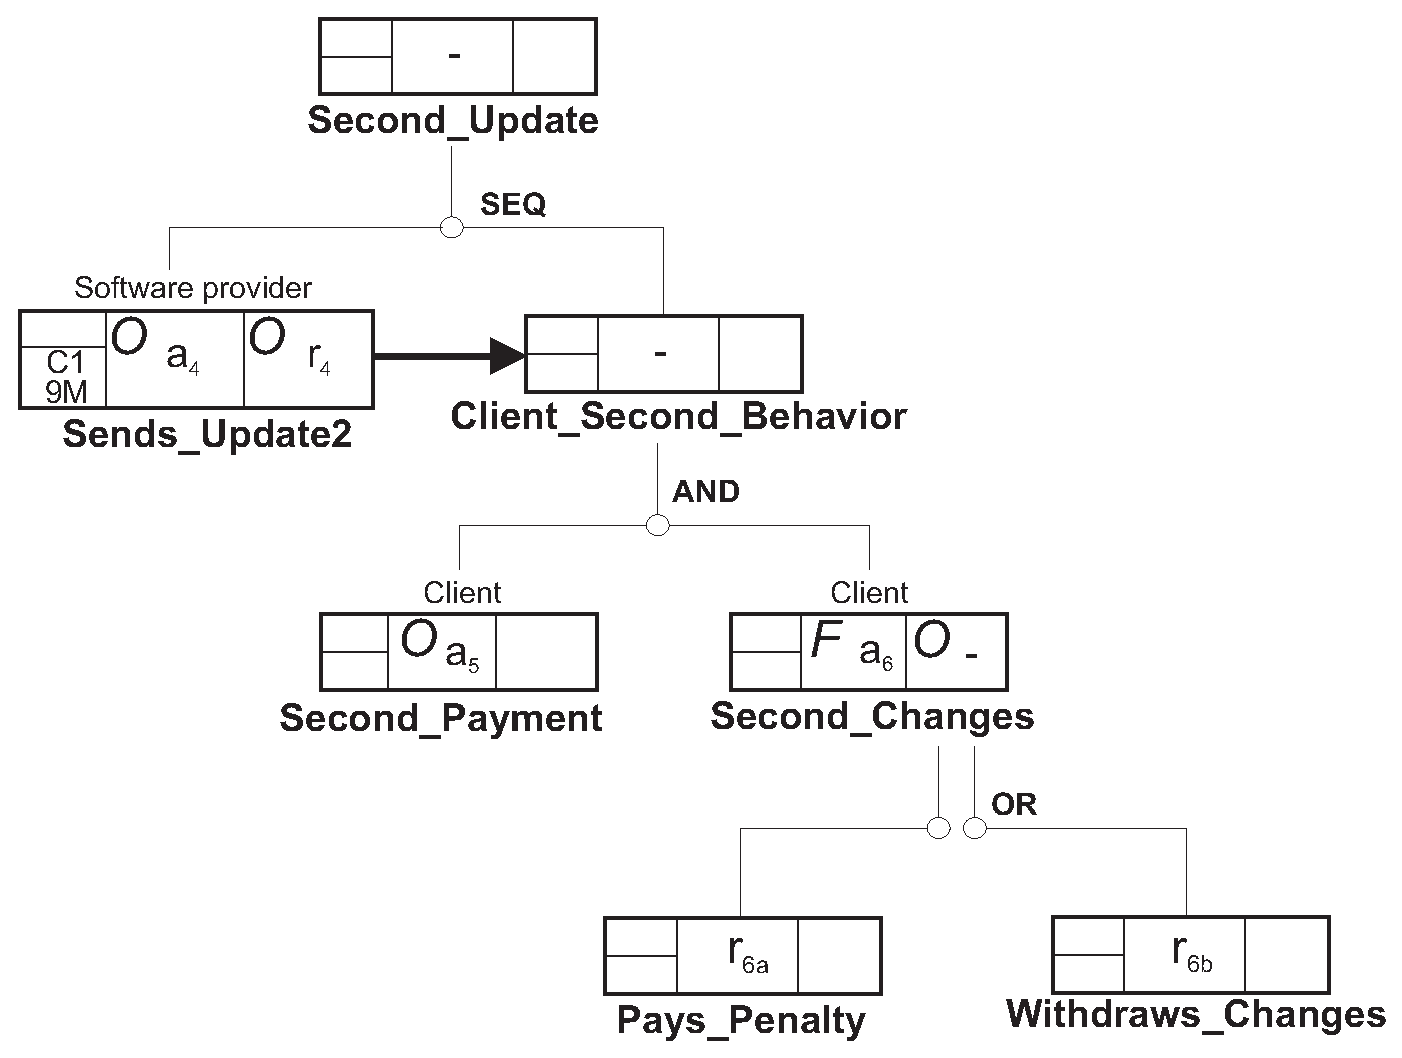
\includegraphics[width=12cm]{Figures/SoftwareSystem3.eps}
%%\end{center}
%%  \caption{Decomposition of clause \textit{Second\_Update}}
%%  \label{SoftwareSystem3}
%%\end{figure}
%%
%%\begin{figure}
%%\begin{center}
%%  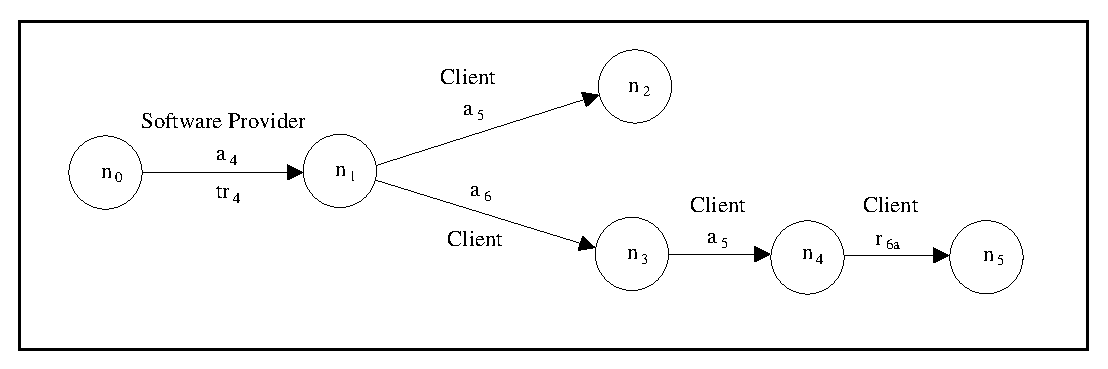
\includegraphics[width=12cm]{Figures/automaton.eps}
%%\end{center}
%%  \caption{Automaton of \textit{Example \ref{exa1}}}
%%  \label{automaton_exa1}
%%\end{figure}
%%
%%We want to see if the timed automaton $\mathcal{A}$ shown in Figure \ref{automaton_exa1} satisfies this contract $C$ starting from its initial location $n_0$, i.e., $(\mathcal{A},n_0) \models C$. First, we can see that what we have on the top of the diagram is a SEQ-refinement where the first subcontract of the sequence states the obligation of performing the atomic action $a_4$. Then, we apply rule \textbf{(4)} in this case, and we see that the initial obligation is fulfilled, performing $Software \, provider$ action $a_4$ in the specified time frame $tr_4$ in the edge from $n_0$ to $n_1$ (and there is no other possible path).
%%
%%Next, we have to see if the remaining sequence of the contract, that we denote as $C_1$, is satisfied by the timed automaton $\mathcal{A}$ from location $n_1$, i.e., $(\mathcal{A},n_1) \models C_1$. Now what we have is an AND-refinement between an obligation and a prohibition, so applying rule \textbf{(10)} we define the satisfaction of this refinement as the satisfaction of the obligation on one hand, and the satisfaction of the prohibition on the other hand, in both cases starting from location $n_1$.
%%
%%In the case of obligation, according to rule \textbf{(1)}, we have to see that action $a_5$ is performed by $Client$ in every possible path from $n_1$. We have two possible paths, $n_1 \flecha{} n_2$ and $n_1 \flecha{} n_3 \flecha{} n_4 \flecha{} n_5$, and in both cases we have an edge performing action $a_5$, so the obligation is satisfied.
%%
%%In the case of prohibition, according to rule \textbf{(3)}, we have to see that action $a_6$ is not performed by $Client$ in any possible path. For path $n_1 \flecha{} n_2$ this statement is fulfilled, but for path $n_1 \flecha{} n_3 \flecha{} n_4$ we have that action $a_6$ is performed in the edge from $n_1$ to $n_3$, so the prohibition is not fulfilled. Nevertheless, as there is a reparation for the subcontract specifying the prohibition, we have to see if this reparation is fulfilled, considering this subcontract eventually fulfilled in that case. Reparation $R_6$ states the obligation of performing action $r_{6a}$ or $r_{6b}$, and we can see that, after applying rules \textbf{(8)} and \textbf{(11)}, it is enough to satisfy the obligation of one of the two actions in order to consider the reparation as fulfilled. We have that the edge from $n_4$ to $n_5$ performs action $r_{6a}$, so the reparation is fulfilled and the subcontract is eventually fulfilled.
%%
%%Therefore, we conclude that contract $C$ is satisfied by timed automaton $\mathcal{A}$.
%%
%%\end{example}
%%
%%%%Example2%%
%%\begin{example}\label{exa2}
%%
%%We consider now the diagram we have in Figure \ref{diagram_exa}. This diagram can be formally written as:
%%\\
%%
%%\noindent $(\epsilon,Box0,\epsilon,\epsilon,(\epsilon,Box1,\epsilon,\epsilon,(Agent1,Box3,\epsilon,\epsilon,O(a),R3)\\
%% 	    And \, (Agent1,Box4,\epsilon,\epsilon,P(b),\epsilon),\epsilon) \, Seq\\
%% 			(Agent2,Box2,\epsilon,\epsilon,O(\epsilon,Box5,\epsilon,\epsilon,c,\epsilon) Or \,
%% 			(\epsilon,Box6,\epsilon,\epsilon,d,\epsilon),\epsilon),\epsilon)$
%%\\
%%
%%\noindent where $R_3$ is the reparation we define for $Box3$, that states the obligation of performing action $e$, formally written as $(\epsilon,Rep3,\epsilon,\epsilon,O(e),\epsilon)$.
%%
%%\begin{figure}
%%\begin{center}
%%  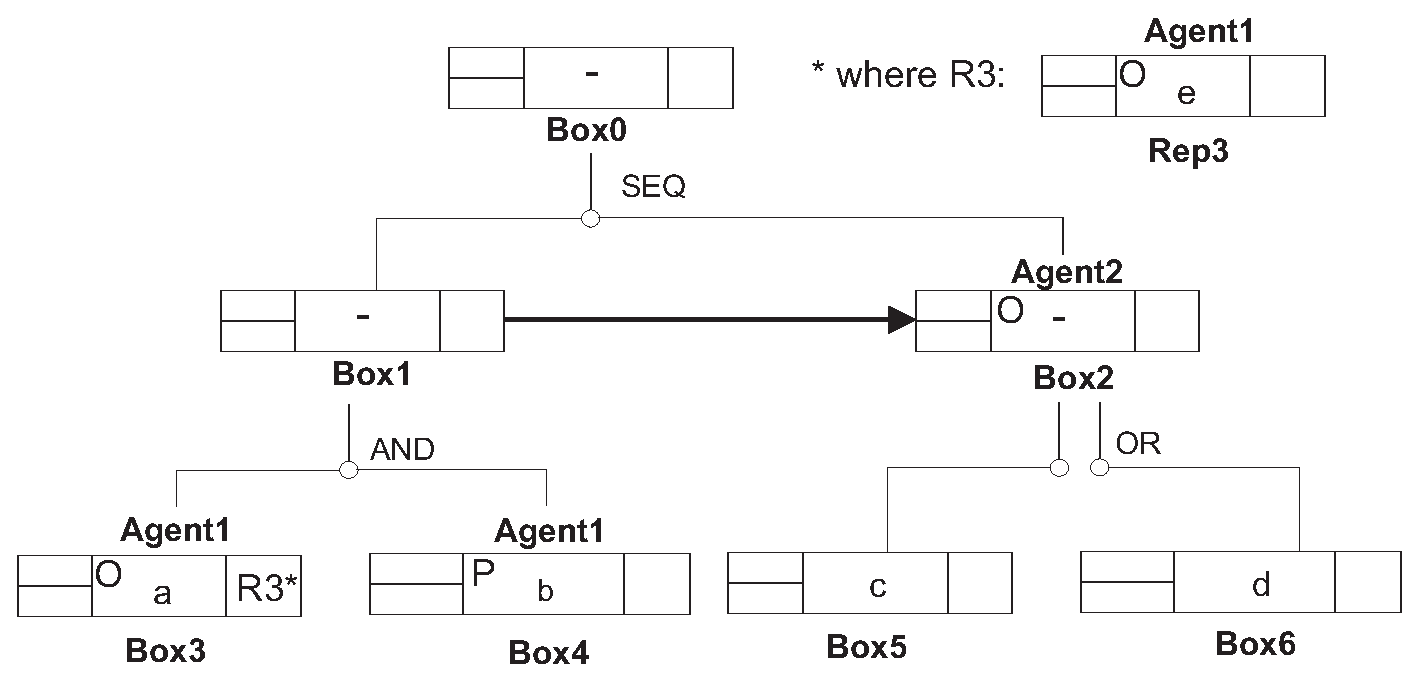
\includegraphics[width=10cm]{Figures/Example2.eps}
%%\end{center}
%%  \caption{\textit{C-O Diagram} of \textit{Example \ref{exa2}}}
%%  \label{diagram_exa}
%%\end{figure}
%%
%%We want to see which one of the timed automata shown in Figure \ref{automaton_exa2} satisfies the contract modelled by this diagram starting from its initial state $n_0$. First, as we have a SEQ-refinement which first element is an AND-refinement with no deontic operator applied over it, we apply rule \textbf{(15)} to distribute SEQ-refinement over AND-refinement, so according to rule \textbf{(10)} the satisfaction of this contract consists of the satisfaction of obligation of $a$ (or its reparation) followed by the obligation of $c$ or $d$, and the permission of $b$ followed by the obligation of $c$ or $d$.
%%
%%\begin{figure}
%%\begin{center}
%%  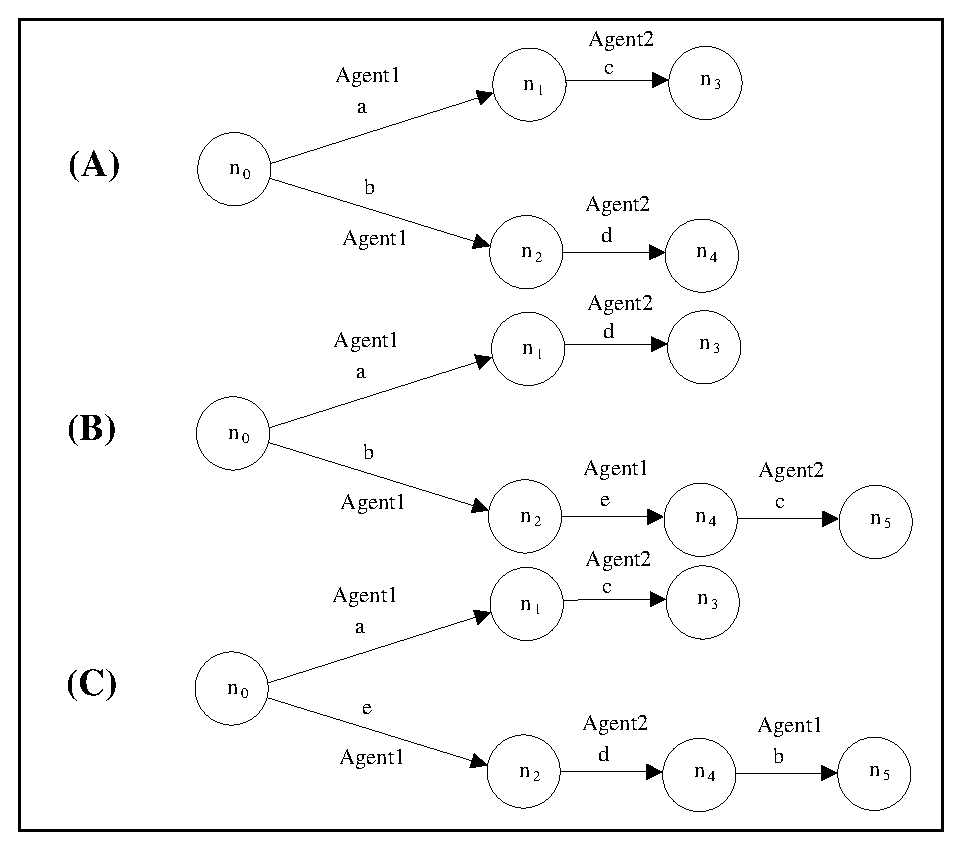
\includegraphics[width=8cm]{Figures/automaton2.eps}
%%\end{center}
%%  \caption{Automata of \textit{Example \ref{exa2}}}
%%  \label{automaton_exa2}
%%\end{figure}
%%
%%For the former subcontract we apply rule \textbf{(4)} and we see that this rule is not satisfied by automaton (A), so it does not satisfy the contract and we do not care about it anymore. In the cases of (B) and (C) action $a$ is performed in path $n_0 \flecha{} n_1 \flecha{} n_3$ and its reparation $e$ is performed in the alternative path $n_0 \flecha{} n_2 \flecha{} n_4 \flecha{} n_5$, so we have to see if starting from the locations we reach after performing these actions the obligation of $c$ or $d$ is satisfied. According to rules \textbf{(8)} and \textbf{(11)} this is equivalent to satisfy obligation of $c$ or satisfy obligation of $d$ and we see that in both cases, (B) and (C), this statement is satisfied.
%%
%%For the latter subcontract we apply rule \textbf{(5)} and we see that in the cases of (B) and (C) action $b$ is performed in path $n_0 \flecha{} n_2 \flecha{} n_4 \flecha{} n_5$, so we have to see if starting from the locations we reach after performing $b$ --$n_4$ in the case of (B) and $n_5$ in the case of (C)-- the obligation of $c$ or $d$ is satisfied. According to rules \textbf{(8)} and \textbf{(11)} this is equivalent to satisfy obligation of $c$ or satisfy obligation of $d$ and we see that in (C) this obligation is not fulfilled, so it does not satisfy the contract. Automaton (B) performs action $c$ after performing $b$, so it is the only automaton that satisfies the contract modelled by the diagram.
%%
%%\end{example}
%%
%%%%Translation from diagrams to CL%%
%%\subsection{From \codiag\ to \CL}
%%
%%%%CL definition%%
%%The contract language \CL\ \cite{Prisacariu2008} enables formal specification of deontic electronic contracts. It is based
%%on a combination of deontic, dynamic and temporal logics, allowing the representation of obligations, permissions and prohibitions, as well as temporal aspects. Moreover, it also gives a means to specify exceptional behaviours arising from the violation of obligations (what is to be demanded in case an obligation is not fulfilled) and of prohibitions (what is the penalty in case a prohibition is violated). CL contracts are written using the syntax shown in Definition \ref{defCLSyntax}.
%%
%%\bdfn\label{defCLSyntax} (\CL\ Syntax) 
%%\begin{center}
%%\begin{tabular}{rcl}
%%    $C$ & $:=$ &  \begin{array}[t]{l}
%%						      C_O \,|\,
%%						      C_P \,|\,
%%						      C_F \,|\,
%%						      C \wedge C \,|\,
%%						      [\beta]C \,|\,
%%						      \top \,|\,
%%						      \bot
%%						      \end{array} \\
%%	  $C_O$ & $:=$ &  \begin{array}[t]{l}
%%							      O_C(\alpha) \,|\,
%%							      C_O \oplus C_O
%%							      \end{array} \\
%%    $C_P$ & $:=$ &  \begin{array}[t]{l}
%%							      P(\alpha) \,|\,
%%							      C_P \oplus C_P
%%							      \end{array} \\
%%    $C_F$ & $:=$ &  \begin{array}[t]{l}
%%							      F_C(\alpha)
%%							      \end{array} \\
%%    $\alpha$ & $:=$ & \begin{array}[t]{l}
%%								      0 \,|\,
%%								      1 \,|\,
%%								      \overline{a} \,|\,
%%								      a \,|\,
%%								      \alpha \,\&\, \alpha \,|\,
%%								      \alpha \,;\, \alpha \,|\,
%%								      \alpha \,+\, \alpha
%%								      \end{array} \\
%%    $\beta$ & $:=$ &  \begin{array}[t]{l}
%%    									\epsilon \,|\,
%%								      0 \,|\,
%%								      1 \,|\,
%%								      \overline{a} \,|\,
%%								      a \,|\,
%%								      \beta \,\&\, \beta \,|\,
%%								      \beta \,;\, \beta \,|\,
%%								      \beta \,+\, \beta \,|\,
%%								      \beta^*
%%								      \end{array} \\
%%\end{tabular}
%%\end{center}
%%\edfn
%%
%%A contract clause $C$ can be either an obligation ($C_O$), a permission ($C_P$) or a prohibition ($C_F$) clause, a conjunction of two clauses, the trivially satisfied contract ($\top$), the impossible contract ($\bot$) or a clause preceded by the dynamic logic square brackets. $O_C(\alpha)$ is interpreted as the obligation to perform $\alpha$ in which case, if violated, then the reparation contract $C$ must be executed. An obligation clause may be an exclusive disjunction of two other obligation clauses. This is interpreted as being obliged to satisfy one of the obligations but not both. In the same way, a permission clause may be an exclusive disjunction of two other permission clauses. This is interpreted as being permitted to perform one of the permissions but not both. $P(\alpha)$ is interpreted as the permission to perform $\alpha$. $F_C(\alpha)$ is interpreted as forbidden to perform $\alpha$ and if $\alpha$ is performed then the reparation $C$ must be executed. $[\beta]C$ is interpreted as if action $\beta$ is performed then the contract C must be executed. The conjunction of two clauses is interpreted as both clauses have to be satisfied. $\epsilon$ is an empty action, $1$ is the action that matches any action, while $0$ is the impossible action. Action expressions ($\alpha$ and $\beta$) can be constructed from basic ones using the operators $\&$, $;$, $+$ and $^*$ where $\&$ stands for the actions occurring concurrently, $;$ stands for the actions to occur in sequence, $+$ stands for a choice between actions, and $^*$ is the Kleene star. $\overline{\cdot}$ is the complement, so $\overline{a}$ means ``any action except $a$''.
%%
%%Here we define a syntactic translation from the diagrams to \CL\ language. However, note that \codiag\  are richer than \CL\ (for instance, there is no time in \CL) and thus the translation necessarily will have to abstract away some of the features of the diagrams. We comment on that later in this section. 
%%
%%%%Informal translation%%
%%
%%The translation of atomic and compound actions is quite straightforward: an AND-refinement in \codiag\ corresponds to the concurrency operator ``$\&$'' in \CL, an OR-refinement in \codiag\ corresponds to the choice operator ``$+$''  in \CL, and a SEQ-refinement in \codiag\ corresponds to the sequence operator ``$;$'' in \CL.
%%
%%Concerning to the application of deontic norms (obligations, permissions and prohibitions) over the actions, in \codiag\ we have that when we write one of these norms in a box, it is applied over all the actions in the descendant boxes (or in the same box). Therefore, the translation into \CL\ just consists of writing the composition of these actions and apply the corresponding deontic norm over it.
%%
%%The translation of the different ways of composing deontic norms in \codiag\ into \CL\ is a bit more complex, specially because there is not sequence operator to compose clauses in \CL\ that can correspond to the SEQ-refinement in \codiag. The other refinements are easier to translate: an AND-refinement composing two deontic norms corresponds to the conjunction operator ``$\wedge$'' between these norms, while an OR-refinement corresponds to the exclusive choice operator ``$\oplus$''. For the SEQ-refinement between two norms we write in \CL\ a conjunction between both norms, but adding the expression $[\beta]$ before the second norm, where $\beta$ is the action under the first norm, so the second norm is only applied after performing this action.
%%
%%Expressing conditions in \CL\ also differs from the way we do it in \codiag. In the diagrams we have a field in the boxes allowing us to specify the conditions, but in \CL\ this is not possible, so we use again the expression $[\beta]$, now before the conditional part of the contract, being $\beta$ the condition that must be fulfilled to take this part of the contract into account.
%%
%%In \codiag\ we have a field in the boxes allowing us to specify real-time restrictions in the contract. Unfortunately, the specification of timing constraints is not yet supported by \CL, so what we do in this case for the translation is encoding these constraints in the definition of the actions they affect. E.g., in \codiag\ we can have a box specifying the obligation of the action ``send an e-mail'' and the restriction ``before 2 hours'' in its specific field in the box. In the corresponding \CL\ translation we have to specify directly the obligation of the action ``send an e-mail before two hours''. We have the same situation for the agents in \codiag, i.e., they have to be encoded in the definition of the actions in \CL.
%%
%%Finally, the translation of reparations from \codiag\ into \CL\ is done directly, since in both cases we just have a reference to the secondary contract that comes into effect when the violation occurs. For that purpose, in \codiag\ we use a field in the boxes containing an obligation or a prohibition where we can specify a reparation, whereas in \CL\ a reference to a reparation must be a subindex of an obligation or a prohibition expression.
%%
%%%%Formal translation%%
%%
%%Formally, we consider a parameterized translation function \FT$_{[agent,TR]}$ from \codiag\ into expressions of \CL. The parameter $agent$ is used to propagate the entity affected by a norm, being empty if it has not been specified yet (we will write only \FT$_{[TR]}$ in that case), and the parameter $TR$ is used to propagate any time restriction we have specified, being initially empty. The result of applying this translation function over the diagrams is shown in Definition \ref{defCO2CL}.
%%
%%\bdfn\label{defCO2CL} (Translation function from \codiag\ to \CL) \\
%%
%%{
%%\scriptsize
%%\begin{equation}
%%\FT_{[TR]}((agent,name,g,tr,O(C),R)) = [g]O_R(\FT_{[agent,TR \cup tr]}(C)) \label{eq1}
%%\end{equation}
%%\begin{equation}
%%\FT_{[TR]}((agent,name,g,tr,P(C),\epsilon)) = [g]P(\FT_{[agent,TR \cup tr]}(C)) \label{eq2}
%%\end{equation}
%%\begin{equation}
%%\FT_{[TR]}((agent,name,g,tr,F(C),R)) = [g]F_R(\FT_{[agent,TR \cup tr]}(C)) \label{eq3}
%%\end{equation}
%%\begin{equation}
%%\FT_{[TR]}(\epsilon,name,g,tr,C,\epsilon)= [g]\FT_{[TR \cup tr]}(C) \label{eq4}
%%\end{equation}
%%\begin{equation}
%%\FT_{[agent,TR]}(\epsilon,name,g,tr,C,\epsilon)= [g]\FT_{[agent,TR \cup tr]}(C) \label{eq5}
%%\end{equation}
%%\begin{equation}
%%\FT_{[agent,TR]}(C_1 \, And \, C_2) = \FT_{[agent,TR]}(C_1) \, \& \, \FT_{[agent,TR]}(C_2) \label{eq6}
%%\end{equation}
%%\begin{equation}
%%\FT_{[agent,TR]}(C_1 \,Or \, C_2) = \FT_{[agent,TR]}(C_1) \, + \, \FT_{[agent,TR]}(C_2) \label{eq7}
%%\end{equation}
%%\begin{equation}
%%\FT_{[agent,TR]}(C_1 \,Seq \, C_2) = \FT_{[agent,TR]}(C_1) \, ; \, \FT_{[agent,TR]}(C_2) \label{eq8}
%%\end{equation}
%%\begin{equation}
%%\FT_{[TR]}(C_1 \,And \, C_2) = \FT_{[TR]}(C_1) \, \wedge \, \FT_{[TR]}(C_2) \label{eq9}
%%\end{equation}
%%\begin{equation}
%%\FT_{[TR]}(C_1 \,Or \, C_2) = \FT_{[TR]}(C_1) \, \oplus \, \FT_{[TR]}(C_2) \label{eq10}
%%\end{equation}
%%\begin{equation}
%%\FT_{[TR]}(C_1 \,Seq \, C_2) = \FT_{[TR]}(C_1) \, \wedge \, [\beta_{C_1}]\FT_{[TR]}(C_2) \label{eq11}
%%\end{equation}
%%\begin{equation}
%%\FT_{[agent,TR]}(a) = a_{[agent,TR]} \label{eq12}
%%\end{equation}
%%}
%%
%%\edfn
%%
%%Lines (\ref{eq1})--(\ref{eq3}) correspond to the translation into \CL\ of a box where we specify an obligation, a permission or a prohibition, considering also any possible reparation. As agents and time restrictions are not yet supported natively by \CL, these two things are encoded as part of the actions, so we propagate them into the translation of $C$ under the deontic norm, joining the time restriction in the box ($tr$) with any other time restriction we could have specified before ($TR$). The conditions are encoded at the beginning of the clause between square brackets, whereas the name of the box is not taken into account.
%%
%%Lines (\ref{eq4})--(\ref{eq5}) correspond to the translation into \CL\ of a box where we do not specify any obligation, permission or prohibition. Again, agents and time restrictions are propagated into the translation of $C$, and the conditions are encoded at the beginning of the clause between square brackets. The difference between these two equations is that in the former $agent$ has not been specified yet, whereas in the latter $agent$ has already been specified, so we have to propagate it.
%%
%%Lines (\ref{eq6})--(\ref{eq8}) correspond to the translation of a refinement when the deontic operator has already been specified and the refinement is used to compose actions, while lines (\ref{eq9})--(\ref{eq11}) correspond to the translation of a refinement when the deontic operator has not been specified yet and the refinement is used to compose deontic norms. The translation is quite straightforward in all the cases except in the case of (\ref{eq11}). As we do not have a sequence operator between deontic norms in \CL, we use the conjunction operator ``$\wedge$'' between both contracts and we write $[\beta_{C_1}]$ before $C_2$ to denote that it is  only applied after performing the actions in $C_1$. These translations are given for refinements composing only two element ($C_1$ and $C_2$) for the sake of simplicity, but they can be easily generalized for any number of elements ($C_1$,$C_2$,\ldots,$C_n$).
%%
%%Finally, line (\ref{eq12}) is the translation of a simple action into \CL. In this case we just have to write the action in \CL\ including in its codification any time restriction and the agent we have propagated from its ancestor boxes ($a_{[agent,TR]}$).
%%
%%There are some limitations in the translation from \codiag\ into \CL, so the syntax of the diagram must be restricted when we want to do it: (i) The recursion we can have over boxes in \codiag\ cannot be translated into \CL, so we can only have recursion in guards, and (ii) the disjunction in \CL\ is only allowed between obligations and permissions, so we cannot write an OR-refinement combining prohibitions nor different kinds of deontic norms if we intend to do the translation.
%%
%%\section{Summary}\label{sumDia}
%%\markright{~\ref{sumDia} Summary}
%%
%%This chapter has presented \codiag, a novel approach for the visual representation of electronic contracts. These diagrams can include the obligations, permissions and prohibitions of the different signatories, the penalties in case of not fulfilment of their obligations and prohibitions, the conditions for the application of certain clauses, and absolute and relative timing constraints.
%%
%%Syntax and semantics have been provided for \codiag\ to make possible the formal analysis of the specified contracts. The semantics consists of a transformation into a network of timed automata that can be implemented in the UPPAAL tool, so this tool can be used for the validation and verification of the electronic contracts.
%%
%%A case study about an online auctioning process e-contract has been developed, showing the application of \codiag\ and how, by means of its semantics, the UPPAAL tool is used for the formal verification of the contract model.
%%
%%Finally, two alternative applications of \codiag\ have been presented: the way of checking if a timed automaton model satisfies the specified contract by means of a set of satisfaction rules, and a function to transform \codiag\ into \CL\ specifications.